\documentclass{report}

\usepackage{style/suthesis-2e}
\copyrightfalse
\signaturefalse

\usepackage[fleqn]{amsmath}
\usepackage{amssymb}
\usepackage{bm}
\usepackage{booktabs}
\usepackage{epigraph}
\usepackage{float}
\usepackage{graphicx}
\usepackage{listings}
\usepackage{mathrsfs}
\usepackage{natbib}
\usepackage{relsize}
\usepackage{subcaption}
\usepackage{url}
\usepackage[hidelinks]{hyperref}
\usepackage{refcount} % allows getting around stupid issues with references in headers + upercasing

\usepackage{tikz}

\usetikzlibrary{shapes,arrows}
\usetikzlibrary{decorations.pathreplacing, decorations.pathmorphing, snakes, calligraphy}

\tikzstyle{block} = [rectangle, draw, thick, align=center, rounded corners]
\tikzstyle{boundingbox} = [thick, lightgray]
\tikzstyle{dashblock} = [rectangle, draw, thick, align=center, dashed]
\tikzstyle{conc} = [ellipse, draw, thick, dashed, align=center]
\tikzstyle{netnode} = [circle, draw, very thick, inner sep=0pt, minimum size=0.5cm]
\tikzstyle{relunode} = [rectangle, draw, very thick, inner sep=0pt, minimum size=0.5cm]
\tikzstyle{line} = [draw, very thick, -latex']
\tikzstyle{arrow} = [draw, ->, thick]

\def\checkmark{\tikz\fill[scale=0.4](0,.35) -- (.25,0) -- (1,.7) -- (.25,.15) -- cycle;}

\definecolor{bpurp}{HTML}{984ea3}
\definecolor{bblue}{HTML}{377eb8}
\definecolor{bgreen}{HTML}{4daf4a}
\definecolor{borange}{HTML}{ff7f00}

% footnote without a marker
\makeatletter
\def\blfootnote{\gdef\@thefnmark{}\@footnotetext} 
\makeatother

\lstset{language=Python,
    frame=single,
    breaklines=true,
    postbreak=\raisebox{0ex}[0ex][0ex]{\ensuremath{\color{red}\hookrightarrow\space}}
}

\restylefloat{figure}
\newcommand{\Prop}{\textbf{Proposition: }}
\newcommand{\Prob}{\textbf{Problem: }}
\newcommand{\Prf}{\textbf{Proof: }}
\newcommand{\Sol}{\textbf{Solution: }}
\newcommand{\grad}{\nabla}
\newcommand{\Nats}{\mathbb{N}}
\newcommand{\Ints}{\mathbb{Z}}
\newcommand{\Rats}{\mathbb{Q}}
\newcommand{\Reals}{\mathbb{R}}
\newcommand{\Comps}{\mathbb{C}}
\newcommand{\Prb}[1]{P\left( #1 \right)}
\newcommand{\PT}[1]{P\left( \text{#1} \right)}
\newcommand{\PCon}[2]{P\left( #1 \mid #2 \right)}
\newcommand{\PConT}[2]{P\left( \text{#1} \mid \text{#2} \right)}
\DeclareMathOperator{\E}{\mathbb{E}}
\DeclareMathOperator{\tr}{\textbf{tr}}
\DeclareMathOperator*{\argmin}{argmin}
\DeclareMathOperator*{\argmax}{argmax}
\newcommand{\thus}{\quad\mathlarger{\mathlarger{\mathlarger{\Rightarrow}}}\quad}
\newcommand{\wght}{\mathbf{w}}
\newcommand{\im}{\text{im }}
%%\newcommand\scalemath[2]{\scalebox{#1}{\mbox{\ensuremath{\displaystyle #2}}}}


%% Tikz stuff
\usetikzlibrary{shapes,arrows}
\usetikzlibrary{decorations.pathreplacing, decorations.pathmorphing, snakes, calligraphy}

\tikzstyle{block} = [rectangle, draw, thick, align=center, rounded corners]
\tikzstyle{boundingbox} = [very thick, gray]
\tikzstyle{dashblock} = [rectangle, draw, thick, align=center, dashed]
\tikzstyle{conc} = [ellipse, draw, thick, dashed, align=center]
\tikzstyle{netnode} = [circle, draw, very thick, inner sep=0pt, minimum size=0.5cm]
\tikzstyle{relunode} = [rectangle, draw, very thick, inner sep=0pt, minimum size=0.5cm]
\tikzstyle{line} = [draw, very thick, -latex']
\tikzstyle{arrow} = [draw, ->, thick]
\tikzstyle{mapsto} = [draw, |->, thick]

\def\checkmark{\tikz\fill[scale=0.4](0,.35) -- (.25,0) -- (1,.7) -- (.25,.15) -- cycle;}


%% Some colors stolen from ColorBrewer
\definecolor{bpurp}{HTML}{984ea3}
\definecolor{bblue}{HTML}{377eb8}
\definecolor{bgreen}{HTML}{4daf4a}
\definecolor{borange}{HTML}{ff7f00}
\definecolor{bred}{HTML}{a50f15}

% footnote without a marker
\makeatletter
\def\blfootnote{\gdef\@thefnmark{}\@footnotetext}
\makeatother



\dept{Psychology}

\begin{document}
\title{Toward understanding human adaptibility with deep learning models}
\author{Andrew Kyle Lampinen}
\principaladviser{Jay McClelland}
\firstreader{Noah Goodman}
\secondreader{Surya Ganguli}
%\thirdreader{Jane Supernumerary} %if needed
%\fourthreader{Severus Snape} %if needed

\beforepreface
\setcounter{page}{4}  % Stanford formatting requirements
\prefacesection{Abstract}

Human cognition is fundamentally flexible --- we can adapt to a novel task without any direct experience on that task, based on its relationship to previous tasks. By contrast, while deep-learning models can achieve superhuman performance on many tasks, they are unable to adapt to even slight task alterations. I begin this dissertation by reviewing the literature on cognitive flexibility, and recent advances in artificial intelligence. I provide a synthesis of these literatures, and outline the challenges that I believe remain. In particular, I focus on the ability to adapt to new tasks zero-shot, that is, without any data.\par
To address this challenge, I propose a general computational framework for modeling adaptation to novel tasks based on their relationship to prior tasks. The framework is based on \emph{meta-mappings}, higher-order tasks that transform basic tasks. I propose a parsimonious implementation of this framework in the form of \emph{homoiconic meta-mapping} architectures. I demonstrate this framework across a wide variety of tasks and computational paradigms, ranging from regression to image classification and reinforcement learning. I compare to both human adaptibility, and language-based approaches to zero-shot task performance. I demonstrate that the model is extremely succesful, often achieveing 80-90\% performance on a novel task that directly contradicts its prior experience. I further show that using this adaptation as a starting point can dramatically accelerate later learning on a task, and reduce the errors made on the way to mastery by nearly an order of magnitude. \par
Thus, I suggest that meta-mapping provides a plausible computational basis for human adaptability and efficient learning. This dissertation therefore provides a framework for building better cognitive models and more flexible artificial intelligence systems. In the final chapter, I review the broader contributions of this work to an ongoing discussion about the computational principles necessary for intelligence, and highlight possible future directions ranging from understanding mathematical cognition to neuroscience. 

\afterpreface

\chapter{Introduction}
\epigraph{``The most elementary single difference between the human mind and that of brutes lies in this deficiency on the brute's part to associate ideas by similarity.''}{William James, \textit{Principles of Psychology}}
Deep learning methods have achieved incredible success recently, reaching human-level performance in domains ranging from vision \citep[e.g.][]{Szegedy2015} to playing games \citep[e.g.][]{Silver2016}. However, these systems still lack some important human abilities \citep[e.g.][]{Lake2016}. Deep learning models are data-hungry, while humans can frequently learn from relatively few examples. Furthermore, even if they are given a large amount of data, deep learning systems may not be able to generalize well outside the data distribution they trained on. Finally, once knowledge is learned in the weights of a deep learning model, it is difficult to flexibly reuse that knowledge. From the perspective of William James (quoted above), most neural networks are brutes, which don't understand the similarity of new situations to their prior experiences, and so do not know how to flexibly respond to changes in their environment or goals. \par
By contrast, humans can use our knowledge flexibly. We can learn from few examples. We can introspect about our learned behavior to explain or change it. We can even remap our behavior in a way completely inconsistent with our prior behavior, such as trying to lose a game we have previously been trying to win \citep{Lake2016}. More generally, we are often able to accurately behave according to linguistic instructions without seeing examples of such behavior. All of these types of flexibility can be quite difficult for deep learning systems. \par 
This apparent contrast between humans and neural networks has raised questions about the validity of neural networks as a cognitive model for many years \citep[e.g.][]{Fodor1988}, and the recent successes of deep learning have only increased the frequency of these critiques \citep[e.g.][]{Lake2015, Lake2016, Lake2017, Marcus2018}. It is important to address these perspectives, and to understand how deep learning systems can be improved to serve as better models of human flexibility. There have been a number of attempts to address or integrate these critiques from a variety of perspectives \citep[e.g.][]{McClelland1999, McClelland2010}. In this paper, I will particularly focus on how these critiques overlook the benefits of transfer \citep{Lampinen2017a} and recent progress in deep learning \citep{Hansen2017}. In particular, deep learning research has made important progress on improving learning speed, generalization, and flexibility. However, even with contemporary methods there are many human-like abilities that remain frustratingly out of reach. \par
In the remainder of this paper, I will attempt to address these issues. I will first review some of the cognitive issues and the progress to date, and try to provide a unifying perspective on how various types of transfer contribute to human learning and flexibility. I will then show some of my prior research on this topic, including analyses of the effects of transfer in neural networks, explorations of flexibility and transfer in humans. Finally, I will propose some new directions for my research, including a set of studies exploring human flexibility in a new setting, and a new type of deep learning architecture that yields much greater flexibility. \par

\section{Area review: Cognitive flexibility}

What kind of flexibility do humans have? We are often able to learn rapidly. For example, we can achieve some competence in a novel video game within a few minutes \citep{Lake2016}. We can learn new concepts from seeing only a relatively small number of examples \citep[e.g.][]{Bourne1970}. We can often learn even faster if we can actively participate in the learning process by selecting examples rather than passively receiving them, especially if the concepts are simple enough that we can generate a good hypothesis space \citep{Markant2014a}. \par
We can then apply what we have learned to new situations. The studies of \citet{Bourne1970} that I referenced above show that once people have learned a new concept from examples, they can generalize that knowedge to learn structurally-similar new concepts more rapidly. Indeed, even without explicit awareness of the relationship between two tasks, humans can sometimes benefit from transfer effects \citep[e.g.][]{Day2011}. In general, human analogical transfer abilities have been suggested to be a critical component of `` what makes us smart'' \citep{Gentner2003}. \par
Yet human flexibility is apparent beyond transfer between isomorphic tasks. We can often competently change our learned behavior in response to instruction or other goals, such as trying to lose a game we were previously trying to win, or trying to achieve some orthogonal task \citep{Lake2016}. Indeed, it has been known for almost a century that even other animals exhibit this sort of flexible knowledge use -- they engage in ``latent learning'' of environmental features that may be useful when solving future tasks \citep{Blodgett1929}. Both humans and other animals are capable of flexibly applying our knowledge in many situations.  \par
However, our flexibility is not universal. Sometimes it is quite difficult for us to integrate new knowledge. For example, even undergraduate students with substantial mathematical background often struggle with understanding new mathematical concepts.\footnote{I will focus on mathematical cognition for much of this paper. Although the phenomena I discuss are much more general, and I will include a number of other examples, mathematical cognition offers a unique microcosm of human abilities for transfer, abstraction and flexibility.} They may mistakenly assume the converse of a theorem, or get caught up in concrete ways of thinking about abstract concepts \citep{Hazzan1999}. Socrates' dialog about doubling the area of a square captures the misunderstandings that modern subjects make, just as it did for those over 2000 years ago, yet it does not help them to deeply understand the principle \citep{Goldin2011}. Even after engaging with the dialog, nearly 50\% of modern subjects failed at the simplest generalization of the principle: to a square of different size. Similarly, even students who complete a course in geometry in high school may not achieve formal deductive understanding of the concepts taught unless (or until) they become undergraduate mathematics majors \citep{Burger1986}. Furthermore, superficial details of how a concept is presented can have profound impacts on how easy it is to reason about, even if the underlying concept is exactly the same \citep[e.g.][]{Kotovsky1985, Kaminski2008, Lampinen2017b}. There is a wealth of research showing that our learning is far from universally flexible. \par 
We also often fail to flexibly use the knowledge we have. For example, even mathematics students who can correctly state a rule or theorem are not necessarily able to apply it to create a proof \citep{Weber2001}. Similarly, even if experimental subjects can learn a basic concept rapidly, it may be difficult for them to apply it in more abstract situations or to extract more formal understanding from it \citep[e.g.][]{Lampinen2017b}. Likewise, rapid analogical transfer is often only possible when superficial details match closely, or when subjects are explicitly told to transfer \citep[e.g.][]{Gick1980}. Because of findings like these, \citet{Detterman1993} has argued that inducing transfer requires manipulations ``with the subtlety of a baseball bat,'' and so we should conclude that ``significant transfer is probably rare and accounts for very little human behavior.'' This is a particularly tendentious presentation of the issues, but it captures the important broader insight that humans are not always rapid learners or flexible reasoners. \par 
How can we reconcile the demonstrations of rapid learning and flexibility with the evidence that some concepts are learned slowly and some knowledge is inflexible? How can we reconcile arguments that transfer is key to ``what makes us smart'' \citep{Gentner2003}, with arguments that ``significant transfer is probably rare and accounts for very little human behavior'' \citep{Detterman1993}? There are a variety of factors that affect whether transfer will occur \citep{Barnett2002, Lampinen2017a}. First, we need high-quality representations of the concepts we are learning in order to reason flexibly with them. These generalizable representations are generally created through making connections between different pieces of our knowledge \citep{Wilensky1991, Schwartz2015}. Second, we often need strategic meta-knowledge about where and how to apply our knowledge in new situations, which also must be learned \citep{Weber2001}. Both these factors mean that transfer may happen more easily over longer periods of time, as I have argued in my prior work \citep{Lampinen2017a}. The quality of the representations we have, and the way those representations relate to the new tasks we are presented with, both affect our ability to learn rapidly and reason flexibly. \par 

\subsection{Flexibility as transfer}
I argue that all these types of flexibility (and inflexibility) can be seen as transfer, defined broadly as the way that ``knowledge acquired in one situation applies (or fails to apply) in other situations.'' \citep{Singley1989}. From this definition it is clear that applying learned features and structures to learn faster in a new situation, as in \citet{Bourne1970}, is a type of transfer. I argue that in fact all rapid learning must rely on transfer of prior knowledge in order to constrain the hypothesis space under consideration. Even other types of flexibility, such as adapting to instructions, can be seen as transferring several different types of knowledge (prior knowledge about a task, other related taks, and language) to a new situation. For example, if we are asked to try to lose at chess, we are essentially presented a new task to which we need to transfer both our prior knowledge of chess and our prior knowledge of what ``trying to lose'' means. Thus flexibility and transfer are essentially two perspectives on the same broad phenomena. I will therefore use these words for different perspectives on this phenomenon. Specifically. I will use ``flexibility'' generally to refer to the behavioral phenomena, and ``transfer'' to refer to the computational principles underlying these phenomena. \par  
Why do we sometimes fail to be flexible? There are several reasons this can occur. First, we may not have the prior knowledge necessary to be flexible. We can't transfer what we don't know. Second, our representations may lack the quality necessary to transfer them. We often can't transfer what we don't know well \citep[c.f.]{Hazzan1999, Weber2001}. Third, we may not recognize that we have applicable prior knowledge to transfer \citep{Detterman1993}. Finally, we may actually have prior beliefs that do not apply to the present situation, and so transferring them will actually interfere with our ability to learn. This is generally called ``negative transfer'' \citep{Singley1989}. \par
For transfer to be beneficial overall, we must generally encounter settings where our prior knowledge is applicable, and furthermore we must have good ways of integrating that prior knowledge with new experiences. In the next section I will discuss some of the features that allow us to do so. \par

\subsection{What factors contribute to our flexibility?}
We need to address the computational question of how and when we can use transfer to behave flexibly. In this section I will give a brief overview of the contributing factors. \par 

\textbf{Complementary learning systems:} First, it has been proposed that we have complementary learning systems \citep{McClelland1995, Kumaran2016}. These complementary systems allow us to learn rapidly from new knowledge while avoiding catastrophic interference \citep{McCloskey1989} with the statistical knowledge we have accumulated over longer timescales. The key idea is that we have a slow (parametric) learning system which sets up good representations, while a fast (nonparametric) learning system stores new knowledge by using these representations. Throughout this paper, we will return to this theme of fast and slow learning which support each other. I will therefore divide the rest of this section into the ``slow'' and ``fast'' systems that contribute to transfer.\par
However, it's worth noting that ``slow'' vs. ``fast'' learning systems is not a strict dichotomy. This broad distinction is useful, but in reality learning systems fall on a continuum, and the time-course of learning in a given system is often dramatically affected by what knowledge is already present \citep[e.g.][]{McClelland2013}. Thus this dichotomy between learning systems should not be interpreted as a strict division. Instead, it is a useful way of highlighting the cooperation between distinct systems that operate across distinct, yet sometimes overlapping, timescales. \par 

\subsubsection{Slow}
In this section I will discuss the slow learning systems that contribute to transfer and flexibility. \par
\textbf{Culture \& education:} One critical contributor to transfer is culture. Our cultures have accumulated knowledge over extremely long time scales that allows us to advance much more rapidly now \citep{Tomasello1993, Bengio2012}. For example, mathematical concepts have been constructed by humans \citep{Hersh1997, MacLane1986}, and it has taken us millenia to construct subjects like calculus. Yet today many students gain fluency with these ideas before they graduate high school. Because culture has set up useful representations for these concepts, we are able to acquire them much more rapidly \citep[e.g.][]{McClelland2016}. Furthermore, culture has set up systems of education that are structured precisely to help us learn rapidly and generalize effectively. \par 
By contrast, if our culture does not represent or highlight certain concepts, we may struggle to reason about them. For example, one Amazonian tribe that lacks words for exact numbers shows substantially impaired ability to do basic tasks involving cardinality, which are interpreted as a fundamental deficit in the ability to represent exact cardinality at all \citep{Gordon2004}. Similarly, although the number line as a spatial representation of number appears relatively universal, cross-cultural and historical studies reveal that it is constructed rather than innate \citep{Nunez2011}. Culture helps set up powerful representations and metaphors for us to learn from. Without these representations, our learning would be substantially slower. \par 
\textbf{Transfer between tasks:} Even if culture has not explicitly highlighted (or engineered) structural relationships between tasks, we can benefit from structural similarity. For example, after learning an artificial grammar, subjects can generalize their knowledge to novel sequences from the same grammar applied to novel symbols \citep[e.g.][]{Tunney2001}. From learning about simple harmonic oscillators in the context of springs, participants can transfer to a superficially unrelated problem about controlling the population of a city \citep[e.g.][]{Day2011}. Because many tasks we perform share deep underlying structures, we can take advantage of transfer to learn faster on new tasks. \par 
\textbf{Grounding, embodiment, and representation quality:} One particular type of transfer that seems to be especially useful is grounding \citep{Barsalou2007}. In particular, conceptual representations often tend to be tied into more basic perceptual-motor systems, e.g. arithmetic in the Approximate Number System \citep{Park2013}, or mathematical (and other) reasoning in gestures \citep{Goldin-Meadow1993, Goldin-Meadow1999}. This sort of grounding can be very beneficial to understanding \citep{Nathan2008, Schwartz2015, Wakefield2018}. Because our perceptual-motor system have exceptionally good representations that are trained over long developmental time-scales, we may benefit from leveraging these representations to transfer our understanding to analogous conceptual domains. \par 
It is also worth considering that grounding and embodiment can hold us back. Even our understanding of symbolic expressions seems to be influenced by ``meaningless'' perceptual details like their spacing \citep{Landy2007}. It has also been argued that too concrete of examples can limit generalization \citep{Kaminski2008}, although the details of that particular demonstration have been debated \citep{DeBock2011, Lampinen2017b}. There is probably some negative transfer from grounding in some cases, but overall it is probably outweighed by the positive. \par
However, there are a number of conceptual issues that come along with grounding, such as how to define abstraction \citep{Dove2016}, and whether the grounding must be in the real-world, or can more generally be in concepts that are better understood \citep{Wilensky1991}, regardless of whether they are basic perceptuo-motor knowledge. The line between grounding and other types of transfer can be blurry, because, like many psychological ideas, its definitions are multifarious. \par 
The overlapping field of embodied cognition has raised the opposite issue, arguing that cognition cannot be considered at all outside of the physical, physiological, and social situations in which it is grounded \citep{Anderson2003}. Others have argued that even the computation metaphor in cognition is fundamentally flawed, because it neglects the fact that intelligence evolved in systems interacting with the world \citep{Cisek1999}, through a process of hierarchically constructed control systems \citep{Cisek2019}. It is important to keep these arguments in mind, and not to neglect the world in which our brains reside in favor of a disembodied, computational mind. \par 
\textbf{Rerepresentation and different kinds of knowledge:} The work of Karmiloff-Smith \citep[e.g.][]{Karmiloff-Smith1986, Karmiloff-Smith1992, Clark1993} focused on the idea that we repeatedly redescribe our internal knowledge, reorganizing it in order to better understand the world. To support this theory, she examined evidence of U-shaped developmental curves, where children would actually get worse at a task before they reached ceiling, often because they at first over-generalized a rule. She argues that this shows a pattern of systematic progression of knowledge from implicit representations to various stages of explicit ones which allow progressively more flexibility. In \citet{Karmiloff-Smith1986} she describes some particularly interesting evidence: children fail to balance an oddly shaped block when asked to do so, but successfully balance it when asked to build a house, because their procedural knowledge is more sophisticated than their explicit knowledge. \par 
This pattern of procedural knowledge proceeding more explicit or object-like knowledge is supported by a much broader literature, from the gesture results of \citet{Goldin-Meadow1993} referenced above to work suggesting that we progress from understanding mathematical concepts as processses to understanding them as objects \citep{Dubinsky1991, Hazzan1999}. If we do not already have good representations for a concept, we must create them by slow, procedural learning and reorganization, before we can begin to reason flexibly with the concept. However, it's worth noting that the process is bidirectional -- procedural knowledge supports conceptual understanding, but conceptual knowledge also helps improve procedural performance \citep{Rittle-Johnson2001}. Furthermore, procedural learning can occasionally be misleading. Getting too caught up in procedures that only work in simple cases can actually inhibit conceptual understanding \citep{McNeil2005}. There are sometimes trade-offs to transfer (see section \ref{fast_slow_interactions}). \par 
Is a separate rerepresentation process necessary to explain these phenomena? It is difficult to determine this. Often rapid transitions and rule-like behavior can be fully captured within neural networks or statistical learning models more generally \citep[e.g.][]{McClelland1999, McClelland2002, Schapiro2009, Aslin2012}. While \citet{Karmiloff-Smith1992} argues that these mechanisms can not explain U-shaped developmental trajectories, since error-correcting learning will not apply where there are no errors, she ignores the potential effects of all the other learning that children are simultaneously doing on other related tasks. Furthermore, some compression emerges naturally from the learning dynamics of gradient descent \citep{Tishby2015, Shwartz-Ziv2017, Achille2017}. It is difficult to rule out the possibility that U-shaped developmental trajectories can be explained by the combination of this compression and the effects of other learning on related tasks. \par
\textbf{Summary:} We accumulate knowledge throughout the course of our lives. Some of this knowledge is implicit in the statistics of the world around us, while some is culturally constructed and transmitted. The quality of our knowledge representations can be improved by connecting to other knowledge, or by grounding in perceptual-motor understanding. Once we have acquired sufficiently high-quality knowledge representations, we are often able to transfer when we encounter a new task, and thereby learn more effectively than we could from \textit{tabula rasa}. This improvement in learning manifests as both more efficient learning and better generalization. \par

\subsubsection{Fast}
In this section I will discuss the systems that contribute to fast learning and transfer. It's important to note that these are systems that can be applied rapidly, but are not necessarily learned rapidly. Indeed, many of these reasoning systems are themselves culturally constructed, and must thus be learned over development. \par
\textbf{Hippocampal:} From the complementary learning systems perspective, the hippocampus serves as a fast learning system which can store an essentially unlimited number of distinct experiences while minimizing interference, i.e. as a nonparametric learning sytem \citep{Kumaran2016}. This makes it an excellent sub-system for learning from a small amount of data, because it can store a few experiences and allow them to be retrieved at a later time. It can also help with integrating this knowledge without catastrophically interfering \citep{McCloskey1989} with knowledge gleaned from prior experiences, by allowing interleaving of these prior experiences in learning \citep{McClelland1995}. This can potentially occur in a usefully biased way \citep{Kumaran2016}. There may even be interesting computations performed within the hippocampus to support certain types of rapid generalization \citep{Kumaran2012}. \par 
\textbf{Interactive learning \& hypothesis testing:} Humans are able to use our stored experiences to rapidly learn. One example of this is that we often behave as though we are formulating and testing hypotheses, even from a very young age \citep{Sobel2004, Gopnik2014}. We can even take advantage of these hypotheses in order to actively acquire information from the world that is most useful for us \citep[e.g.][]{Markant2014a}. By using our prior knowledge of the world to help interpret new experiences, we are able to make extremely fast inferences about how to understand a new situation. \par
\textbf{Education \& learned flexibility:} However, our ability to reason rapidly is not solely learned on our own. Indeed, a focus of education is preparing us for future learning \citep{Bransford1999}, and flexibility \citep[e.g.][]{Richland2012}. That is, we are explicitly taught to learn increasingly rapidly as education goes on. Elementary school children require months or years of rote practice to learn arithmetic, but college mathematics students are expected to hear a theorem once and then immediately be able to apply it. As noted above, we may not be perfect at these faster learning tasks \citep[e.g.][]{Hazzan1999}. However, adults are much better at them than children, and mathematics graduate students are much better than undergraduates \citep{Weber2001}. The ability to learn and apply new knowledge rapidly develops as we do.Furthermore, as we grow up we also grow better at explaining our actions, and adapting to instructions \citep[e.g.][]{Doebel2015}. Over the course of development, we practice many types of flexibility. \par 
\textbf{Explanations and demonstrations:} Both in education and outside of it, explanations are a key way we learn about the world, because they can succinctly convey rich structure \citep[e.g.][]{Keil2006, Lombrozo2006}. Importantly, explanations can be succinct because they exploit our prior knowledge in order to convey only the information that needs to be clarified (i.e. they follow the pragmatic principle of not being overinformative, expressed by \citet{Grice1975} for communication more generally). We not only learn from hearing explanations, but also from producing them \citep{Chi1989, Chi1994}, and so it is a common pedagogical principle to ask students to generate explanations. Explanations form a key tool for learning. \par
Similarly, we can also learn quite rapidly from demonstrations, which provide another succinct means for conveying important structure in the world. This learning requires applying our prior knowledge to infer what should and should not be generalized, but fortunately we can do this even from a young age, see \citet{VanDamme2002} for example. Both explanations and demonstrations provide powerful tools for learning rapidly. We develop the ability to exploit these tools early in life \citep{Carpenter2005}. \par 
\textbf{Analogical and relational reasoning, and abstraction:} Some researchers have argued that analogical transfer and abstraction form crucial components of our learning \citep[e.g.][]{Gentner2003, Lakoff2008, Gentner2017}. These accounts often focus on fast, explicit transfer of the form explored by \citet{Gick1980}, for example. The structure-mapping algorithm \citep{Falkenhainer1989} proposed for this is based on explicitly searching over possible isomorphisms, which tends to be infeasible in practice. However, there may be ways to implement it efficiently enough that it could be considered for complex cognitive models \citep{Forbus2017}, and in past work I suggested that implicit learning could provide heuristics to dramatically speed up this search \citep{Lampinen2017a}. It's also reasonable to expect this ability to be related to education and other individual factors, since its been observed that features such as fluid intelligence may interact with the type of scaffolding provided to affect explicit analogical transfer \citep{Kubricht2017}. Indeed, older students are often better at transferring knowledge than younger ones \citep[e.g.][]{Chen1999}. This is suggestive of this type of transfer being a learned skill, rather than a cognitive primitive. \par
Much of the work on analogical and relational reasoning also focuses on the benefits of comparing multiple examples, which can lead to more reliable induction of abstractions or schemas and better transfer \citep{Gick1980, Gentner2017}. It has even been suggested that this is a key way to understand the benefits of grounding \citep{Jamrozik2016}. However, in some past work, I found that seeing two different presentations of a mathematical concept lead to better learning overall than seeing either individually, but did not lead to significantly better abstraction of formal principles \citep{Lampinen2017b}. Thus it remains important to ask when reasoning about multiple examples leads to abstraction, and when it does not. One feature that is often important is explicitly considering the relationship between examples \citep{Gentner2017}, but it's likely that the quality of understanding of the examples matters as well. \par 
\textbf{Consciousness and explicit reasoning:} Consciousness is a slippery topic, but unfortunately must be discussed, as it underlies many of the fast-learning systems above. Most of these rely on our ability to explicitly reason about concepts once we have sufficiently high-quality representations of them. The global workspace theory of consciousness \citep{Baars2005, Dehaene2017} is closely aligned  to this perspective. It states that conscious knowledge is precisely that which is globally accessible, and therefore with which we are most flexible. This concords to some degree with the perspectives of \citet{Karmiloff-Smith1986}, who argued that once we re-represent knowledge to be explicit, we can use it more flexibly. \par
However, \citet{Karmiloff-Smith1986} also argued that there were different levels of explicit representation of knowledge, and indeed some consciousness researchers have proposed more graded transitions from implicit to explicit \citep[e.g.][]{Cleeremans2002}. Computational models of graded transistions have been proposed, where explicit knowledge is essentially learned by a separate system which reasons over implicitly learned representations \citep{Cleeremans2014}. This fits more with the work reviewed above showing a graded transition to explicit knowledge built upon implicit understanding grounded in percetual-motor features \citep[e.g.][]{Goldin-Meadow1993}, procedures \citep[e.g.][]{Hazzan1999}, or more basic concepts \citep{Wilensky1991, Patel2018}. Thus, when thinking about the relationship between implicit and explicit knowledge is unavoidable, we will take the perspective that explicit reasoning is built upon implicitly learned representations. \par 
Another place where explicit reasoning plays a role is in helping us to understand and learn from our own mistakes. For example, \emph{deliberate practice} (targeting specific aspects of performance for improvement) has been claimed to be key to developing expertise \citep{Ericsson1993, Ericsson2017}. Yet to engage in deliberate practice requires meta-knowledge about what needs to be improved, and indeed this abstract understanding is an important component of expert knowledge \citep{Feltovich2012}. \par
\textbf{Summary:} We possess fast learning systems that are engineered by evolution, such as the hippocampus, and ones that are culturally transmitted, such as our ability to follow instructions in our native language(s). Together, they allow us to infer a great deal from little information, by leveraging our slowly-accumulated prior knowledge. They also allow us to flexibly adapt our behavior through practiced algorithms like following instructions. \par 

\subsubsection{Interactions between fast and slow learning systems} \label{fast_slow_interactions}
I claim that most transfer arises as a synergy between different kinds of learning across different timescales. In particular, the knowledge we have accumulated over our lifetimes (part of which has been accumulated by our cultures over millenia) allows us to constrain the hypothesis space for new learning, so that we can make accurate inferences from a few examples in a new situation. \par 
From my perspective, this slowly-learned knowledge of the world can take multiple forms. It can occur in the mapping from inputs to our awareness, for example in visual cortex neurons which adapt to the regularities encountered over development \citep{Barlow1975}. However, it can also occur in the systems that implement higher-level and more rapid computations.\footnote{Clearly certain kinds of knowledge will lend themselves more easily to being learned in development and others will lend themselves more easily to being culturally transmitted or even learned by evolution. For the most part, I will generally assume that this knowledge emerges from experience or is culturally conveyed rather than being built in \citep{Hansen2017}, but my conclusions will mostly be agnostic to the origins of any particular piece of knowledge.} For example, the results on transfer in artificial grammar learning described above \citep{Tunney2001} or the results on transfer of simple harmonic oscillator strategies \citep{Day2011} show that humans are able to transfer knowledge at the level of structures or algorithms. The limits of this transfer are as yet unclear, as are the time-scales over which different kinds of transfer can occur; some of the work in my dissertation will attempt to explore these issues.\par  
\textbf{Limitations \& tradeoffs:} Of course, there are trade-offs to relying on transfer and prior knowledge. When new tasks are not well aligned with our prior knowledge, relying on prior knowledge can actually interfere with learning. For example, this is one piece of the argument that we made \citep{Lampinen2017b} to explain the results of \citet{Kaminski2008}. This is an illustration of the broader phenomenon of negative transfer -- interference effects produced by transferring between non-isomorphic domains. A wide variety of studies have observed this type of phenomenon \citep[e.g.][]{Luchins1942, Landrum2005}. Our prior knowledge can be detrimental in some situations. \par
This brings us back to the broader point raised by \citet{Detterman1993} above, that humans are often unable to efficiently or flexibly transfer knowledge to new situations. Instead, this must be a goal of education \citep{Bransford1999}, and learning what is transferable may require developmental time \citep{Lampinen2017a} if the representations of the tasks are not sufficiently good to support faster transfer. We can be efficient and flexible when our prior learning has set us up to be. We are not always. We can be mislead by mismatches between the past and the present, or we can simply fail to find the correct analogy.\par

\subsection{Steps towards flexibility in deep learning}

A great deal of recent work in machine learning can be seen as attempts to build machine-learning systems with greater flexibility. In particular, much of this work has tried to allow them to learn from fewer examples, or generalize better to data that weren't seen during training. This work typically follows one of two approaches. The first, multi-task learning, focuses on learning multiple tasks with a single model, in the hope that the additional constraints on the model's representations will cause it to learn more rapidly or generalize better. The second approach, meta-learning, focuses on learning how to learn tasks, in the hopes of learning much faster and generalizing better from extremely small samples. I will give a brief overview of both these literatures in this section. \par

\subsubsection{Multi-task learning}

Multi-task learning is generally related to the ``slow'' learning systems I described in humans. Typically, parameters are partially shared between the two tasks, and these shared parameters are learned over long time-scales. This can be done either in a sequential fashion (where you use one task to pre-train the network for another), or simultaneously (where you learn multiple tasks at the same time or on alternating gradient steps). Auxiliary tasks need not be of the same type as the main task, for example reinforcement learning tasks can be supplemented with auxiliary supervised tasks like temporal autoencoding \citep[e.g.][]{Hermann2017}, or unsupervised tasks can be used to pre-train for supervised ones \citep[e.g.][]{Wu2018}. \par
\textbf{Pre-training:} One example of sequential multi-task learning is the extremely common practice of pre-training a network on some canonical task in order to use one of its hidden layers as a feature for some other related task. For example, pre-training on ImageNet \citep{Deng2009} is often seen as a useful general feature extractor for vision tasks \citep{Huh2016}, even for quite different transfer domains \citep[e.g.][]{Marmanis2016}. There is still active research on how to optimally pre-train features for various goals \citep[e.g.][]{Wu2018}. \par    
However, pre-training is used on more than just vision tasks. In natural language processing (NLP) applications, the representations of words is often pre-trained on co-occurrence prediction tasks \citep[e.g.][]{Pennington2014}. The more general language modeling task (predicting words conditioned on past input) can serve as unsupervised pretraining for many tasks \citep[e.g.][]{Radford2019}. In AlphaGo \citep{Silver2016}, the networks were pre-trained to predict expert go-players' moves, and then were tuned from that starting point using reinforcement learning. The principle that pre-training a network can allow it to generalize better from smaller training sets appears to be quite general, although there is still some debate and ongoing research \citep[e.g]{He2018, Silver2017}. \par
There are also many remaining questions about how other features of training interact with transfer. Some researchers have argued that \emphe{disentangled representations} will be helpful for future tasks \citep{Higgins2018}, while others have argued that disentangled representations are hard to define, and that the evidence that they are useful is weak \citep{Locatello2019}. Other some recent work suggests that some forms of regularization may actually harm transfer \citep{Kornblith2019}. One possible explanation for this is that regularization is too compressive in the transfer setting -- it may compress away some real features that are useful for the transfer task, but not for the source task. However, this might be different if the tasks were trained simultaneously (see below) rather than in a pre-training setting. Understanding when this occurs, and how to balance the generalization benefits of regularization with transfer benefits will be an important area for future work. \par

\textbf{Curriculum learning:} A more general kind of pre-training is curriculum learning \citep{Bengio2009} -- the idea that training models on a structured progression of tasks can improve generalization. Pre-training on a single task is essentially a very simple curriculum. The idea of curricula began with \citet{Elman1993}, but was debated \citep[e.g.][]{Rohde1997}. However, subsequent work has demonstrated the importance of curricula both in toy settings \citep{Gulcehre2013} and in much more complicated models \citep[for example][discussed below]{Graves2016}. \par
Curriculum learning of course raises another issue: what if you want your model to perform well at several tasks? If you switch to training on a new task, it may catastrophically interfere with your ability to perform a previous task \citep{McCloskey1989}. The complementary learning systems perspective \citep{McClelland1995, Kumaran2016} was intended in part to address this issue. A number of other approaches have also been proposed recently, based on ideas like preserving parameters from updates proportionally to how important they are for old tasks \citep{Kirkpatrick2016}, or learning tasks separately but distilling the knowledge into a single network later \citep{Rusu2015}, or by trying to use unsupervised learning to find compact representations and allocate new tasks so that they don't interfere \citep{Achille2018a}. There are also some memory-based approaches discussed in section \ref{meta_learning_sec} that can ameliorate this problem. Thus there are a variety of approaches that can address catastrophic interference, while still maintaining the benefits of curriculum learning. \par

\textbf{Simultaneous multi-task learning:} However, many multi-task learning approaches train on the tasks simultaneously rather than sequentially. For example, simultaneously training a natural language translation system to do image captioning in the target language improves its translation performance \citep{Luong2016}. Even training it to translate between multiple language pairs is beneficial \citep{Dong2015}. This can even lead to zero-shot generalization to translation between language pairs never seen together in training \citep{Johnson2016a}. \par 
The idea of multi-task learning has proven even more critical in Reinforcement Learning (RL), where auxiliary tasks have been suggested as a key approach to overcoming the problem of reward sparsity \citep[e.g.][]{LeCun2016}. They have been used this way on a variety of RL tasks, for example in grounded language learning \citep{Hermann2017}. \par
The broad observation that deep networks will learn representations that represent shared structure in the tasks they perform, and can exploit this shared structure to generalize better, is not new. It was observed at least as long ago as \citet{Hinton1986}, and has continued to intrigue researchers since \citep[e.g.][]{Lampinen2017a}. In particular, it is a key feature that separates deep networks from simpler statistical learning architectures, and allows them to uncover and exploit deep structure in the world \citep{Rogers2008}. This is key to some of the kinds of transfer that deep networks demonstrate, and has been substantially helpful in the machine learning work above. Thus the benefits of multi-task transfer should not be neglected when considering deep learning models of cognition. \par 

\textbf{Learning which parameters to share:} Most the work above simply fixes architectures with pre-specified shared and unshared weights. However, there are other approaches that attempt to learn which weights to share. The work of \citet{Achille2018a}, referenced above, is one example of this.  Other authors have considered using evolutionary algorithms to decide which subsets of modules should be shared \citep{Fernando2017}. Some other approaches can also be seen from this perspective, for example choosing a sparse subset of modules for each forward pass \citep{Shazeer2017} or using a HyperNetwork to generate the weights for other networks \citep{Ha2016}. Both these can be seen as a way of learning which weights should be shared or separate between different ``sub-tasks'' of a task. Some of the work discussed in section \ref{meta_learning_sec} can also be viewed as learning what parameters should be shared and which should be separate. While in principle a fully-shared network could learn which parameters to share just by gradient descent, in practice a more structured approach to this problem can be useful. \par 

\textbf{Summary:} To summarize, curriculum and multi-task learning can help set up representations that allow deep learning models to generalize better from less data, or to learn tasks that would not otherwise be learnable. This is because the additional constraints imposed by auxiliary or pre-training tasks on the networks representations help it to uncover the true underlying structure in the world. While multi-task learning does not support all the kinds of flexibility that humans demonstrate, it is a key piece of the puzzle of how deep networks can learn faster and generalize better. \par

\subsubsection{Meta-learning \& related approaches} \label{meta_learning_sec}

The fundamental insight of meta-learning is that there is a continuum between data and tasks. We can interpret each (input, target) tuple as a simple task, and we can interpret subsets of a dataset as sub-tasks, for example all the dog images contained within ImageNet form a semantically distinguishable sub-task of the overall task. Analogously, we can often interpret a single task as being just a point in a larger space of tasks. Most meta-learning models exploit these insights by having the architecture adapt to a given task within its activations instead of its weights, just as a CNN would adapt to the fact that its current input was a dog image rather than a tree image within its activations. Learning to adapt to new tasks in this way has been shown to allow for much more efficient learning on new tasks, and may be key to modeling human intelligence \citep{Hansen2017}. \par 
\textbf{Basic meta-learning:}
The basic meta-learning approach (representing a task within activations) has been applied to many settings. For example, it has been used to learn to classify new images based on single positive exemplars of each class \citep{Vinyals2016}. It has also been used to teach recurrent networks to solve simple reinforcement learning problems \citep{Duan2016, Wang2016a, Stadie2018}. \par
There have been many variations on this approach. Some meta-learning work has exploited both slow and fast weights with some success \citep[e.g.][]{Munkhdalai2017}, taking one perspective on the dichotomy I proposed above. Many approaches have exploited other tricks that are broadly useful in machine learning. For example, some work has leveraged unlabelled examples along with a few labelled ones to yield better meta-learning results \citep[e.g.][]{Ren2018}. Other work has shown that attention-based models are useful \citep{Reed2017}, as in many other machine-learning applications \citep[e.g.][]{Vaswani, Gregor2015}. \par
\textbf{Memory-based:} There are a variety of meta-learning approaches that are based on a non-parametric memory, and generally some form of key-value attentional lookup over it. A general extension of the basic meta-learning approach to the case with memory is given in \citet{Santoro2016}. Other approaches are based on using memory only at testing, e.g. by tuning the network rapidly to perform well on similar examples, as proposed by \citet{Sprechmann2018}. \par 
More flexible variants have also been proposed. For example, the differentiable neural computer (DNC), proposed by \citet{Graves2016} is able to receive a graph structure as inputs, learns to store it in memory, and then learns to use that stored information to solve problems like computing shortest paths. This can effecetively be seen as meta-learning -- the architecture has the flexibility to learn and reason from new knowledge rapidly. However, this flexibility remains fundamentally within the computations done for a task which is slowly learned, and does not by itself allow the more general flexibility that humans exhibit. \par
\textbf{Language:} There is some work that has explored related problems from a language-based perspective. For example, \citet{Larochelle2008} considered the general problem of behaving in accordance with language instructions as simply asking a model to adapt its response when conditioned on different ``instruction'' inputs. More recently, there has been a productive line of research in using language to compose network modules for question answering \citep{Andreas, Andreasa}. There has also been some work on reinforcement learning systems that learn to follow natural language instructions in a simple enviroment \citep{Hermann2017}. \par
More recently, \citet{Radford2019} showed that a language model trained on an extremely large corpus of curated websites actually acquires some meta-like abilities, for example the ability to translate languages ``zero-shot'' (i.e. when conditioned on examples of translation pairs and then given a new sentence, it produces a translation). It is also able to summarize, answer questions, etc. It does this presumably because the corpus contains some translation pairs in context or summaries on a page, and so those tasks essentially compose a small part of the language modeling problem. It's worth noting that the performance on these tasks is rudimentary, and far from models that are trained for these tasks in a supervised way, but it is still an impressive demonstration of the power of prediction to extract deep latent structure in the world, and the power of broad enough training data distributions to teach flexibility. \par  
\textbf{Demonstrations:} The issue of learning from demonstrations has also been considered in the machine learning literature for some time, because of its potential applications in problems where we know what behavior we want, but not how to encode it. There the problem has generally been referred to as ``inverse reinforcement learning'' \citep{Ng2000}, i.e. the problem of inferring a value function from observed behavior. A large number of approaches to this problem have been proposed \citep[e.g.][]{Ng2000, Abbeel2004}. Recently, approaches combining meta-learning and deep learning have achieved some success on this. For example, \citet{Finn2016} present an algorithm which can learn to infer a reasonable approximation of the objective function from a single demonstration. This work shows that neural networks can learn to learn from demonstrations. \par
\textbf{Relational and analogical reasoning:} There are a number of other approaches that attempt to explicitly build relational priors or abstraction into deep-learning architectures. Relation networks \citep{Santoro2017} build in this prior by having the architecture explicitly relate different parts of the input, and achieve better performance on answering relational questions about visual scenes. Architectures that directly allow for true relational binding can be beneficial for a variety of applications, especially natural language processing or symbolic reasoning \citep[e.g.][]{Smolensky1990, Smolensky2014, Huang2017}. More generally, graph-structured networks or other relational inductive biases have been suggested as a promising direction in deep learning \citep{Battaglia2018}. How relational inductive biases can benefit learning is an important direction for future research. \par 
However, relational reasoning is constrained by training as well as the architecture. For example, choosing the negative examples that a network learns from to explicitly contrast relational hypotheses can help to yield more relational reasoning \citep{Hill2019}. Exploring how architecture and training interact to produce relational reasoning will be an important future direction. \par
\textbf{Abstraction:} There has also been some work on explicitly building in abstraction capabilities to machine learning systems. For example, in reinforcement learning the idea of options \citep{Sutton1999} and hierarchical reinforcement learning more broadly \citep[e.g.][]{Botvinick2009} are essentially encapsulations of temporal abstraction, where a sequence of actions can be represented as a single higher-level action. For example, we can think of going to the office as a single action, rather than a sequence of many steps. Similar attempts have been made to allow deep learning models to share knowledge across tasks, with some success \citep[e.g.][]{Tessler2016}. \par 
There have also been a variety of attempts to combine deep learning methods with more programming-like approaches. For example, Neural Programmer-Interpreters \citep{Reed2015} essentially endow a recurrent network with the ability to call sub-routines, and a stack of memory for these sub-routines to use. Applying these ideas to meta-learning problems has been reasonably successful, especially with carefully chosen algorithms for integrating knowledge across tasks \citep[e.g.]{Devlin2017}. Similar techniques have been applied to many domains, such as learning from demonstrations \citep[e.g.][]{Xu2017a}. Combining the old ideas of cognition as executing symbolic programs \citep{Newell1961} with the techniques of deep learning can yield improvements in flexibility. \par  
However, most of these methods are still not as universally flexible as humans. The number of abstractions is usually fixed, often abstractions cannot be composed from other abstractions, and abstractions are inflexible to other demands. For example, a system that has learned an option for walking to a goal will not necessarily be able to change to running to the goal without learning this option from scratch. Thus there are still limitations to these approaches at present. \par 
\textbf{Other work:} There is a variety of other work that has exploited different perspectives on meta-learning. Some of this work could be useful for thinking about flexibility. For example, \citet{Finn2017a} proposed Model-Agnostic Meta Learning (MAML), an approach based on optimizing the model so that it could adapt well to a new task in a few gradient steps, and this work has led to many follow-ups \citep[e.g.][]{Finn2017, Finn2018}. \citet{Xu2018} proposed using meta-learning to adapt hyperparameters of reinforcement learning algorithms across tasks. Both of these approaches allow for better adaptation to new tasks or environments. \par
In addition, there has been some work showing that basic neural network models can adapt rapidly to new data that is consistent with prior knowledge, simply by optimizing weights specific to that data while freezing the remaining weights of the network \citep{Rumelhart1993}. This approach only works if there are weights that are specific to the new item(s), so it is not a general kind of flexibility. Nevertheless, this approach has been applied to understand human semantic cognition \citep{Rogers2004}. More recently, I applied it to one-shot and few-shot learning of words in a language-modeling task \citep{Lampinen2018a}. Thus under some circumstances this approach can yield a certain kind of flexibility, even at the scale of large machine learning tasks. This is more evidence of the general point that information which is consistent with prior knowledge can be rapidly integrated \citep{McClelland2013}. \par 
\textbf{Unintentional ``flexibility'':} There has also been some interesting work on flexibility that emerges accidentally under standard training of deep learning systems. In particular, adversarial examples \citep{SzegedyAdv} are cases when adding a very small perturbation to an input can radically alter the network's output. This is a kind of flexibility, but it is not the desired kind. Instead, these appear to be evidence for the fact that deep networks are inherently chaotic systems, which can respond in surprisingly sensitive ways to their inputs. However, it's worth noting that humans can be susceptible to more extreme adversarial perturbations derived on deep networks \citep{Elsayed2018}. Furthermore, adversarial examples can be exploited, e.g. for better training \citep{Goodfellow2015}. \par 
\citet{Elsayed} demonstrated an even more interesting type of unintentional flexibility: deep networks can be ``reprogrammed'' by an input to solve a different task.\footnote{Although not one completely unrelated to the main task the network was trained on -- the network was trained on a vision task, and their reprogrammed tasks were just other vision tasks. It would be interesting to explore the limits of this ``reprogrammability.''} This is a step closer to the flexibility that humans have, but the ``reprogramming'' inputs have to be derived via an optimization process, and tend to be uninterpretable. Thus there is no systematicity in this flexibility. However, my interpretation of these results is that they are encouraging evidence that these models have the capacity to be extremely flexible under appropriate conditions. All that is needed is to train this flexibility to be more systematic. \par  
\textbf{Summary:} To summarize, meta-learning has made progress on several fronts. It is starting to solve the small data problem, by allowing networks to learn efficiently from a small number of examples \citep[e.g.][]{Wang2016a}. At the other extreme of very large data, deep networks can generalize to some extent to tasks which are only hinted at by the trained task distribution \citep[e.g.][]{Radford2019}. However, there are a number of key features of human flexibility that remain to be explained. In the next section, I will relate transfer and flexibility in humans and deep networks, and discuss what features are still missing. \par 

\subsection{Relating flexibility in humans and neural networks}

The encouraging progress on multi-task and meta-learning in recent years suggests that cognitive models exploiting these techniques may help explain human flexibility and transfer \citep{Hansen2017}. In this section, I will attempt to relate the aspects of human and network flexibility that I outlined in the previous sections. \par 
First, it generally seems that the division between fast and slow transfer is applicable both to the machine learning literature (meta-learning vs. multi-task) and to human transfer, as we highlighted above \citep[and in prior work, namely][]{Lampinen2017a}. Following complementary learning systems, I suggest that broadly our slow learning of structure in the world happens over the course of developmental time in a multi-task fashion. Algorithmically, this occurs because parameters in our brain come to represent and exploit structural similarities across the many tasks we experience. We also practice doing fast learning over these slowly-learned representations, in educational settings as well as in everyday experience more broadly. Thus I think that cognitive models should employ both slowly-learned shared representations, and a system that allows for rapid and flexible reasoning over them. I argue that incorporating both aspects will be key to modeling the full range of human flexibility. \par 
It is also important to note the differences between the systematic, structured training that humans encounter in culturally-constructed educational systems, and the unstructured, IID training that deep learning models canonically receive. While curriculum learning addresses some of the sequential learning in education, and meta-learning addresses part of the learning-to-learn aspect, the full training on flexibility is generally missing. For example, humans learn a great deal from explaining as well as simply doing, yet we rarely train our machine learning models to explain their actions. Given the sensitity to training data that both humans and neural networks display, we cannot expect deep learning models to capture human behavior completely under drastically different learning regimes. How to train deep models in more human-like ways is an important direction for future work.  \par
In summary, I think deep learning models remaining promising cognitive models. They have successfully modeled a wide range of phenomena ranging from low-level neural activity to cognition. Furthermore, they are compelling models in particular of high-level cognitive phenomena, because they are some of the only systems to successfully achieve human performance at difficult tasks like visual recognition or playing go. They even have some inherent (if often unstructured and unintentional) flexibility, as indicated by adversarial examples and reprogramming. \par
I suggest that humans are similarly flexible. I suggest that the reason our flexibility is less chaotic is that we learn over the course of development and education to exploit our flexibility in systematic ways, in order to be adaptable to new tasks and situations. A very weak example of this in machine learning is given by \citet{Radford2019}, discussed above, where training a language model on a large enough text distribution gives some generalization to related tasks. However, this network required far more training than could be assumed for humans, and still lacked some of the flexibility that humans have. I suggest that this is because of the lack of multiple tasks to constrain the representations, the lack of an architecture explicitly designed to allow synergies between fast and slow learning, and the lack of the systematic, structured training that humans experience. \par 

\subsubsection{What's still missing?}

For the reasons highlighted above, some flexibility is still missing from deep-learning systems. Although they can often learn a new task from few examples, most demonstrations of this have involved sampling tasks that are within a dense region of the training task distribution. Furthermore, humans have a great deal more flexibility than simply learning rapidly. We can decide how to behave on a new task based on natural language instructions we are given. We can also adapt our behavior on a task based on feedback about our actions, and can jointly learn from language and examples better than we can learn from either alone. \par
We can also remap our behavior on tasks based on instructions or examples of tasks. For example, if we are told to try to lose a game we have previously been trying to win, this is an easy task for us. It would be quite difficult for any contemporary reinforcement learning model to invert its value function. If we are given examples of task mappings, e.g. we've played chess on a smaller board and checkers on a smaller board, we are able to remap our strategies for go to play on a smaller board. That is, we can flexibly map between behavioral strategies on different tasks based on either linguistic or (task) exemplar input. The meta-learning systems I have reviewed do not yet have this flexibility. \par
This is related to the more general point that humans have the ability to flexibly reason across levels of abstraction. For example, humans can relate between examples of a concept and what they imply about the overall concept, e.g. as counter-examples to universal properties. With training, we can even reason flexibly across complex hierarchies of abstraction, as when thinking about the mathematical concepts of numbers, sets, functions, and categories. We are able to recursively build abstractions on top of abstractions (though this is often a slow process). By contrast, deep learning models typically represent different levels of abstraction separately, e.g. at separate layers of a feed-forward architecture. This limits the flexibility of reasoning between them (the only available mapping is the canonical transformation given by the weights), and because the abstraction is built in to the architecture, it can not be applied recursively. Similarly, we can reason both about data and the computations we perform over data, whereas most deep learning architectures restrict their knowledge of computations to weights which they have no explicit access to. This limits the flexibility and representational capacity of these networks. \par 
To summarize, we can flexibly map between data, language, and tasks, across different levels of abstraction. Contemporary deep learning architectures lack this full range of flexbility, although certain models have achieved some promising steps toward certain aspects of it. In section \ref{eml_sec}, I will propose a new architecture that I think comes closer to achieving human-like flexibility. In the remainder of section \ref{RR_sec}, I will describe some past work and future directions that explore the extent of this human flexibility, and work investigating the benefits of multi-task learning in neural networks. \par 

\chapter{Meta-mapping} \label{chapter:zero_shot_via_homm}
\blfootnote{Some of the material in this chapter originally appeared as a workshop paper in the Learning Transferable Skills Workshop at NeurIPS 2019.}
\epigraph{``In the human, internal representations become objects of cognitive manipulation.''}{Annette Karmiloff-Smith,\\\textit{Beyond Modularity}}


As noted in the introduction, humans have the ability to transform our behavior on a task, in accordance with a change in goals. For example, if we are told to try to lose at poker, we can perform quite well on our first try, even if we have always tried to win previously. If we are shown an object, and told to find the same object in a new color or texture, we can do so. How can we adapt our behavior so drastically, without any data on the new task, even when our new goal contradicts all our prior experience? We can do so by exploiting the relationship between the adapted version of the task and the original. In this chapter, I propose a computational model of this adaptation, and demonstrate its success across a variety of domains. Our model is both useful for understanding the flexibility of human cognition, and for designing artificial intelligence systems with more human-like flexibility.   

The model incorporates several key insights into human cognition. First, when performing a task (such as playing poker), humans are aware of what we are doing and why. We propose that this awareness is mediated by an internal representation of the task. Our model therefore performs tasks from a task representation. We take inspiration from various approaches from the machine learning and cognitive science literature, and construct task representations from examples via meta-learning \citep[e.g.][]{Vinyals2016, Santoro2016, Finn2017a, Finn2018, Stadie2018, Botvinick2019}, or from a natural language instruction \citep{Larochelle2008, Hermann2017, Hill2019a}. The model then uses this task representation to respond in a task-appropriate way to its inputs (and for other purposes, such as identifying attributes of the tasks). 

To implement the task computations, we allow a great deal of input processing (perception) to be shared across different tasks. If a human is playing cards, much of the perception of the cards will be identical whether the game is poker or blackjack or bridge, and the task-specific computations will be performed over abstract features such as suit and rank relationships. We thus allow the system to learn a general basis of perceptual features over all tasks with a domain. The system then uses these features in a task-specific way in order to perform task-appropriate behavior. Specifically, the model uses its representation of the current task to parameterize this computation over the perceptual features, and then decodes the result through an output system which is also shared across the tasks. 

We also allow the model to transform its representations of tasks, to accomodate task alterations. We refer to these transformations of tasks as \textbf{meta-mappings}. Meta-mappings allow the model to adapt to a new task \emph{zero-shot} (i.e. without requiring any data from that new task), based on the relationship between the new task and prior tasks. For example, meta-mappings could be used to switch to losing at poker, based on knowledge of poker, and what ``losing'' means across other games. Meta-mappings can be cued either by examples of the meta-mapping applied to other tasks, or by an instruction, just as basic tasks can be inferred from examples or instructions. 

Our model infers and implements these task transformations using the same architetural components that are used to perform the basic tasks. Using the same architectural components for basic tasks and meta-mappings is parsimonious,as it does not require adding new networks for each new type of transformation. Furthermore, it reflects our theory that the brain reuses the same sytems for computations at different levels of abstraction. This may be key to the human ability to repeatedly build abstractions on top of prior abstractions \citep{Wilensky1991, Hazzan1999, Lampinen2017b}, allowing, in principle, for recursion upon our own cognitive processes. Finally, it relates to the computational notion of ``homoiconicity.'' A homoiconic programming language is one in which programs can be manipulated within the language as data. Our implementations are therefore homoiconic, in the sense that tasks can be transformed just like data can. We refer to these architectures as \textbf{homoiconic meta-mapping} (HoMM) architectures. These architectures allow for computational adaptibility that is closer, at least in some ways, to that exhibited by humans.  

The main contributions of this chapter are to propose meta-mapping as a computational framework for understanding task adaptation, and to propose a parsimonious implementation of this framework in the form of homoiconic meta-mapping. In this chapter we will demonstrate the success of our approach in a simple proof of concept domain, and explore some features of its performance. In subsequent chapters, we will compare to human adaptation and show the success of our approach across a variety of tasks, ranging from visual classification to reinforcement learning. See below for a discussion of related work. To our knowledge, this is the first work that proposes transforming a task representation in order to adapt to task alterations zero-shot. 


\section{Task transformation via meta-mappings} \label{sec:HoMM:metamappings}

\textbf{Basic tasks are input-output mappings:} We take as a starting point the construal of basic tasks as mappings from inputs to outputs. For example, poker can be seen as a mapping from hands to bets, chess as a mapping of board positions to moves, and object recognition as a mapping from images to labels. This perspective is common across machine learning approaches, which generally try to infer a task mapping from many examples, or meta-learn how to infer it from fewer examples. In our work, we infer these mappings either from examples, from natural language instructions, or by transforming a prior task mapping. 

\textbf{Tasks can be transformed via meta-mappings:} We propose meta-mappings as a computational approach to the problem of transforming a basic task mapping. A meta-mapping is a higher-order task, which takes a task representation as input, and outputs a representation of the transformed task. For example, we might have a ``lose'' meta-mapping. If given poker as an input, the lose meta-mapping would output a losing variation of poker. If given blackjack, it would output a losing variation of blackjack. If we have such a meta-mapping, we can use it to transform a task in order to perform the transformed version of the task. This allows a model to adapt to a transformed task without having any data on it, just as humans are able to easily switch to trying to lose at a game they have only tried to win in the past. 

How can a meta-mapping be constructed? There is an analogy between meta-mappings and basic task mappings -- they are both simply functions from inputs to outputs. Thus to construct a meta-mapping that we use analogous approaches to those we use for constructing basic task representations. In particular, we infer a meta-mapping from examples (e.g. winning and losing at a set of example games), or natural language (e.g. ``try to switch to losing''). We can then apply this meta-mapping to other basic tasks, in order to infer losing variations of those tasks. Importantly, the system is able to generalize to new meta-mappings, just as it can generalize to new basic tasks. 



\section{Homoiconic meta-mapping architectures} \label{sec:HoMM:architecture}

\begin{figure}[htbp]
\centering
\begin{tikzpicture}[auto]
%% a) constructing
\draw[boundingbox, draw=gray, fill=white] (-8, -2.5) rectangle (-0.25, 2.5);

%% from language
\node[gray] at (-6.5, 2.1) {Instructions};
\node at (-6.5, 1.25) (language) {``Play poker.''};

\node[gray, text width=2cm, align=center] at (-3.5, 2.1) {Language network};
\node[block] at (-3.5, 1.25) (languagenet) {\(\mathcal{L}\)}; 
\path[arrow] (language.east) -- ([xshift=-3]languagenet.west);

\node[bpurp, text width=2cm] at (-0.5, 1.25) (languagetaskrep) {\(z_{task}\)}; 
\path[arrow] ([xshift=3]languagenet.east) -- (languagetaskrep.west);


%% from examples

\node[gray, text width=2.5cm, align=center] at (-6.5, -0.2) {Task examples (encoded)};
\node at (-6.5, -1.25) (examples) {
\(\left\{
\begin{matrix}
({\color{bgreen}z_{hand_{1}}}, {\color{bgreen}z_{bet_{1}}})\\
$\vdots$
\end{matrix}\right\}\)};

\node[gray, text width=2cm, align=center] at (-3.5, -0.4) {Example network};
\node[block] at (-3.5, -1.25) (examplenet) {\(\mathcal{E}\)}; 
\path[arrow] (examples.east) -- ([xshift=-3]examplenet.west);

\node[bpurp, text width=2cm] at (-0.5, -1.25) (examplestaskrep) {\(z_{task}\)}; 
\path[arrow] ([xshift=3]examplenet.east) -- (examplestaskrep.west);

%% b) performing 
\draw[boundingbox, draw=gray, fill=white] (0.25, -2.5) rectangle (8, 2.5);
\node[bpurp] at (1, 1.25) (taskrep) {\(z_{task}\)};

\node[gray, text width=2cm, align=center] at (3, 2.1) {Hyper network};
\node[block] at (3, 1.25) (hypernet) {\(\mathcal{H}\)}; 
\path[arrow] (taskrep.east) -- ([xshift=-3]hypernet.west);

\node[text width=0.5cm] at (0.7, -1.25) (inputs) {\includegraphics[width=0.5cm]{2-HoMM/figures/2_of_spades.png}\\\includegraphics[width=0.5cm]{2-HoMM/figures/4_of_hearts.png}};

\node[gray, text width=2cm, align=center] at (1.9, -0.4) {Perception network};
\node[block] at (1.9, -1.25) (perceptionnet) {\(\mathcal{P}\)}; 
\path[arrow] (inputs.east) -- ([xshift=-3]perceptionnet.west);

\node[bgreen] at (3.2, -1.25) (handrep) {\(z_{hand}\)};
\path[arrow] ([xshift=3]perceptionnet.east) -- (handrep.west);

\node[bblue, block, dashed] at (4.5, -1.25) (tasknet) {\(\mathcal{T}\)}; 
\node[bblue, text width=2cm, align=center] at (4.5, -2) {Task network};
\path[arrow] (handrep.east) -- ([xshift=-3]tasknet.west);
\path[arrow, out=0, in=90] ([xshift=3]hypernet.east) to ([yshift=3]tasknet.north);


\node[bgreen] at (5.65, -1.25) (betrep) {\(z_{bet}\)};
\path[arrow] ([xshift=3]tasknet.east) -- (betrep.west);

\node[gray, text width=2cm, align=center] at (6.8, -0.4) {Action network};
\node[block] at (6.8, -1.25) (actionnet) {\(\mathcal{A}\)}; 
\path[arrow] (betrep.east) -- ([xshift=-3]actionnet.west);

\node at (7.7, -1.25) (output) {\bf \$};
\path[arrow] ([xshift=3]actionnet.east) -- (output.west);

\end{tikzpicture}
\begin{subfigure}{0.5\textwidth}
\caption{Constructing a task representation.}\label{fig:HoMM_architecture:constructing_basic}
\end{subfigure}%
\begin{subfigure}{0.5\textwidth}
\caption{Performing a task from its representation.}\label{fig:HoMM_architecture:performing_basic}
\end{subfigure}
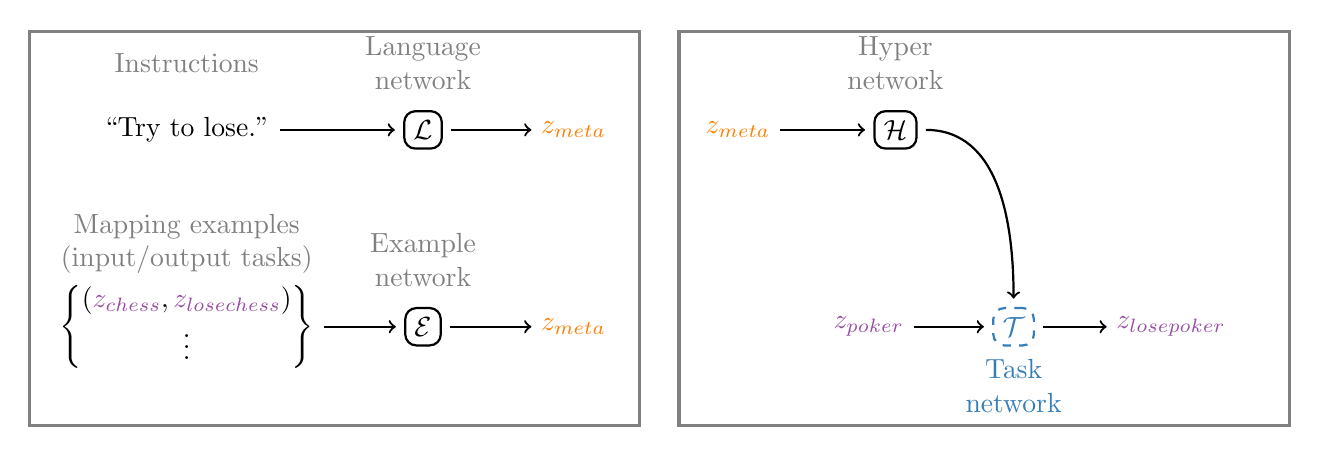
\begin{tikzpicture}[auto]
%% a) constructing
\draw[boundingbox, draw=gray, fill=white] (-8, -2.5) rectangle (-0.25, 2.5);

%% from language
\node[gray] at (-6, 2.1) {Instructions};
\node at (-6, 1.25) (language) {``Try to lose.''};

\node[gray, text width=2cm, align=center] at (-3, 2.1) {Language network};
\node[block] at (-3, 1.25) (languagenet) {\(\mathcal{L}\)}; 
\path[arrow] (language.east) -- ([xshift=-3]languagenet.west);

\node[borange, text width=2cm] at (-0.5, 1.25) (languagetaskrep) {\(z_{meta}\)}; 
\path[arrow] ([xshift=3]languagenet.east) -- (languagetaskrep.west);


%% from examples

\node[gray, text width=3.5cm, align=center] at (-6, -0.2) {Mapping examples (input/output tasks)};
\node at (-6, -1.25) (examples) {
\(\left\{
\begin{matrix}
({\color{bpurp}z_{chess}}, {\color{bpurp}z_{lose chess}})\\
$\vdots$
\end{matrix}\right\}\)};

\node[gray, text width=2cm, align=center] at (-3, -0.4) {Example network};
\node[block] at (-3, -1.25) (examplenet) {\(\mathcal{E}\)}; 
\path[arrow] (examples.east) -- ([xshift=-3]examplenet.west);

\node[borange, text width=2cm] at (-0.5, -1.25) (examplestaskrep) {\(z_{meta}\)}; 
\path[arrow] ([xshift=3]examplenet.east) -- (examplestaskrep.west);

%% b) performing 
\draw[boundingbox, draw=gray, fill=white] (0.25, -2.5) rectangle (8, 2.5);
\node[borange] at (1, 1.25) (taskrep) {\(z_{meta}\)};

\node[gray, text width=2cm, align=center] at (3, 2.1) {Hyper network};
\node[block] at (3, 1.25) (hypernet) {\(\mathcal{H}\)}; 
\path[arrow] (taskrep.east) -- ([xshift=-3]hypernet.west);

\node[bpurp] at (2.66, -1.25) (handrep) {\(z_{poker}\)};

\node[bblue, block, dashed] at (4.5, -1.25) (tasknet) {\(\mathcal{T}\)}; 
\node[bblue, text width=2cm, align=center] at (4.5, -2) {Task network};
\path[arrow] (handrep.east) -- ([xshift=-3]tasknet.west);
\path[arrow, out=0, in=90] ([xshift=3]hypernet.east) to ([yshift=3]tasknet.north);

\node[bpurp] at (6.5, -1.25) (output) {\(z_{lose poker}\)};
\path[arrow] ([xshift=3]tasknet.east) -- (output.west);


\end{tikzpicture}
\begin{subfigure}{0.5\textwidth}
\caption{Constructing a meta-mapping representation.}\label{fig:HoMM_architecture:constructing_meta}
\end{subfigure}%
\begin{subfigure}{0.5\textwidth}
\caption{Transforming a task via a meta-mapping.}\label{fig:HoMM_architecture:performing_meta}
\end{subfigure}
\caption[Performing and transforming tasks with the HoMM architecture.]{Performing and transforming tasks with the HoMM architecture. (\subref{fig:HoMM_architecture:constructing_basic},\subref{fig:HoMM_architecture:constructing_meta}) The HoMM architecture performs basic tasks and meta-mappings from a task representation, which can be constructed from appropriate language inputs or examples. (\subref{fig:HoMM_architecture:performing_basic},\subref{fig:HoMM_architecture:performing_meta}) The task representation is used to parameterize a task network which executes the appropriate task mapping. To do this parsimoniously, the HoMM architecture exploits a deep analogy between basic tasks and meta-mappings --- both can be seen as mappings of inputs to outputs, although they have different types of inputs and outputs. To overcome this challenge, the architecture uses type-specific models to embed all basic inputs, as well as tasks and meta-mappings, in a shared representational space. Thus all tasks and meta-mappings can be seen as transformations applied to entities in this space, which can be executed by shared systems. The parallels between the basic tasks and meta-mappings are reflected in the parallels between the top and bottom rows of the figure.} \label{fig:HoMM_architecture}
\end{figure}

We propose homiconic meta-mapping (HoMM) architectures as an implementation of a system that can perform tasks, and adapt to task alterations via meta-mappings. In this section, we describe the architecture and training process. See Appendix \ref{appendix:model_hyperparameters} for full architecture specifications, training details, and hyperparameters. 

\textbf{Constructing a task representation (Fig. \ref{fig:HoMM_architecture:constructing_basic}):} When humans perform a task, we need to know what the task is. In our model, we specify the task using a task representation. Just like humans, our model supports several different ways of cueing a task, such as instructions, examples of appropriate behavior, or memory of performing the task in the past. Specifically, at different times we either construct a task from natural language, from a dataset of (input, target) tuples for the desired task, or we recall a cached task representation. To construct a task representation from language, we process the language through a deep recurrent network (LSTM). This is similar to techniques used in other work \citep[e.g.]{Hermann2017,Oh2017a,Hill2019a}. To construct a task representation from examples, we process the examples individually to construct appropriate representations for each example, and then aggregate across them by taking an element-wise max. (This provides a nonlinear and dataset-order-invariant way of combining examples --- we found other methods such as averaging performed similarly.) This aggregated representation then receives further processing to produce the task representation. This approach shares some common elements with other approaches used for meta-learning \citep{Garnelo2018}. 

\textbf{Performing a task from its representation (Fig. \ref{fig:HoMM_architecture:performing_basic}):} Once we have a task representation, we need to use it to perform the task. We allow a large part of the input processing (perception) and output processing (action) to be shared across the tasks, so that the task-specific computations can be relatively simple and abstract. This idea is related to the long-standing notion that deep networks (both artificial and biological) will construct more disentangled representations of the task relevant features in deeper layers \citep{Dicarlo2007, Erhan2010}, and is used in a number of meta-learning approaches \citep[e.g.]{Vinyals2016}. We use a HyperNetwork \citep{Ha2016} which takes as input the task representation, and adapts the parameters of a task network. Specifically, the HyperNetwork adapts the values of learned ``default'' connection weights, to make the network task-sensitive. The adapted network then transforms the perceptual features into task-appropriate output features, which can then be decoded to outputs via the shared output processing network. The whole model (including the construction of the task representations) can be trained end-to-end, just as a standard meta-learning system would be. (There are other possible architectures; we show that our approach outperforms the simple alternative of concatenating a task representation to an input embedding before passing it through a fixed network in Supplemental Figures \ref{supp_fig:HoMM_arch_cond_vs_hyper} and \label{supp_fig:extending:RL:arch_cond_vs_hyper}.) 

\textbf{Transforming task representations via meta-mappings (Fig. \ref{fig:HoMM_architecture:constructing_meta}-\subref{fig:HoMM_architecture:performing_meta}):} Above, we defined a meta-mapping to be a higher-order task, which takes as input a task representation, and outputs a transformed task representation. Because our model constructs task representations to perform the tasks, all that we need to implement is a way of transforming these representations to perform a meta-mapping. To do so, we exploit the functional analogy between basic-tasks and meta-mappings, noted above. We can infer a representation for a mapping from examples of the meta-mapping, or from a language description, just like we infer a basic task representation from examples or language. We can then use this meta-mapping representation to parameterize a meta-mapping-specific network that can be used to transform other task representations. This is analogous to how we used a basic-task representation to parameterize a network specific to that task, which could then be used to perform the task. (In Section \ref{sec:HoMM:vector_analogies_inadequate} below, we prove that a simpler approach of using vector analogies for meta-mapping is inadequate.) 

We exploit this analogy by using exactly the same networks for inferring a meta-mapping representation from examples or language as we do for inferring a task representation. We use exactly the same hyper network to parameterize a meta-mapping-specific network as we use to parameterize the task-specific network. That is, we use precisely the same architecture (and default weights that are modulated by the same hyper network) for both basic task computations and meta-mappings. To do so, we assume that the shared perceptual processing embeds individual data points into a representation space that is shared with that used for task representations and meta-mapping representations. This means that all task- or meta-mapping-specific computations can be seen as operations on objects in the same space, and can be inferred identically regardless of the objects being transformed. This is parsimonious, homoiconic, and reflects aspects of the Global Workspace Theory of consciousness \citep{Baars2005}, see discussion.   

\textbf{Training \& evaluating the model:} To train the system to perform the basic tasks, we can compute a task-appropriate loss at the output of the action network, and then minimize this loss with respect to the parameters in all networks. This includes the networks used to construct the task representation, and even the representations of the examples or language that they receive as input. That is, we train the sytem end-to-end to perform the basic tasks. When constructing a task representation from examples, we do not allow the example network to see every item, in order to force the system to generalize, in a standard meta-learning fashion. For example, if the basic task is poker, the system will have to construct a task representation from some hands that will be useful for playing other hands. This ensures that the task representations capture the structure of the task, rather than just memorizing the provided examples. 

To train the system to perform meta-mappings, we try to match the output task representations to those constructed when actually performing those tasks. Specifically, we apply an \(\ell_2\) loss to the difference between the output embedding and the embedding constructed when performing the target task. For example, if the system has been trained to play winning and losing variations of blackjack, we would take the task representation for winning blackjack as input, and try to match the output to the task representation for losing blackjack. Again, when we construct a meta-mapping representation from examples of the mapping, we force it to generalize to other examples. Regardless of how the meta-mapping representation is constructed, we can then test this generalization by passing in the representation for a task like poker, that has never been used for any training on this meta-mapping (either as an example or for generalization). We take the output task representation produced by the meta-mapping, and actually perform the task of losing poker with it. This is how we perform all evaluation of the meta-mapping approach in this paper.

In meta-mapping, generalization is possible at different levels of abstraction. The paragraph above refers to basic generalization --- applying a meta-mapping seen during training to a basic task that meta-mapping has not been applied to during training, in order to perform a held-out basic task zero-shot. However, if the system has experienced sufficiently many meta-mappings during training, we can also test its ability to generalize to held-out meta-mappings. For example, if the system has been trained to switch various pairs of colors in a classification task (red for blue, green for yellow, etc.), it should be able to generalize to switching held-out pairs (red for yellow, green for blue, etc.) from an appropriate cue (examples or instructions). This is an important part of human adaptibility --- we are not only able to adapt tasks via meta-mappings that we understand well, but we can infer and use new meta-mappings based on specific instructions or examples. We will demonstrate this ability in the subset of our experimental domains where we can instantiate sufficiently many meta-mappings. 

\textbf{Comparing to language-based generalization:} Natural language instructions are an important part of how humans are able to generalize to a new task, and prior work on zero-shot performance has often assumed a description of the task as input \citep[e.g.]{Larochelle2008}. For example, a system that has learned to behave in accordance with instructions like ``win at poker,'' ``win at blackjack,'' and ``lose at blackjack,'' should be able to generalize to ``lose at blackjack,'' given sufficiently many training tasks. This, too, does not require data on the novel task. However, transforming the task representation via a meta-mapping may be a more useful inductive bias that allows the system to transform the prior task representation in a targeted way. We thus compare our meta-mapping approach to an approach that simply constructs task representations from language. We show in subsequent chapters that meta-mapping results in better performance on the new tasks, especially when the held-out tasks are very different from trained ones (e.g. directly contradicting). That is, in our experiments, meta-mapping generally has better sample-complexity in terms of the number of prior tasks it must have experienced to perform well. This is crucial, because humans have not seen 95\% of the possible task space when they need to generalize to a new setting.

\section{Experiments}

Meta-mapping is an extremely general framework. Because the assumptions are simply that the basic tasks are mappings from inputs to outputs, and that meta-mappings transform basic tasks, the approach can be applied to most paradigms of machine-learning with only minor modifications. We demonstrate the success of meta-mapping in four settings over the next few chapters, ranging from regression to classification to reinforcement learning. We summarize the contributions of the different experiments in Table \ref{table:HoMM_experiment_summary}. In this chapter, we explore the performance of meta-mapping in detail in a proof-of-concept polynomial domain. We also describe some interesting behavior of the model that may intrigue researchers in cognitive control (but is not a focus of the remainder of the dissertation). 

\begin{table}
\centering
\begin{tabular}{|cp{2cm}|p{2cm}ccp{1.8cm}p{1.5cm}|}
\hline
\textbf{Chapter} &\textbf{Experiment} & \textbf{Motivation} & \begin{minipage}[t]{2cm}\centering\textbf{Held-out MMs}\end{minipage} & \begin{minipage}[t]{1cm}\centering\textbf{Lang. Comp.}\end{minipage} & \textbf{Paradigm} & \textbf{Input}\\[1.3em]
\hline
\ref{chapter:zero_shot_via_homm} & Polynomials & Proof of concept & \checkmark & & Regression & Vector (\(\mathbb{R}^4\))\\[0.5em] 
\ref{chapter:human} & Card games & Comparison to humans & & \checkmark & Regression & Several-hot vector\\[0.5em]
\ref{sec:extending:rl} & Reinforce-ment\phantom{blah} learning & Cognitive and AI relevance & & \checkmark & RL & \(91 \times 91\) RGB image\\[0.5em]
\ref{sec:extending:concepts} & Visual\phantom{blah} concepts & Cognitive and AI relevance & \checkmark & \checkmark & Classification & \(50 \times 50\) RGB image\\[0.5em]
\hline
\end{tabular}

\caption[The contributions of our four sets of experiments.]{The contributions of our four sets of meta-mapping experiments. Our results span various computational paradigms and various degrees of input complexity, and are motivated by both cognitive and AI relevance.} \label{table:HoMM_experiment_summary}
\end{table}

\subsection{Polynomial regression}
\begin{figure}[htbp]
\centering
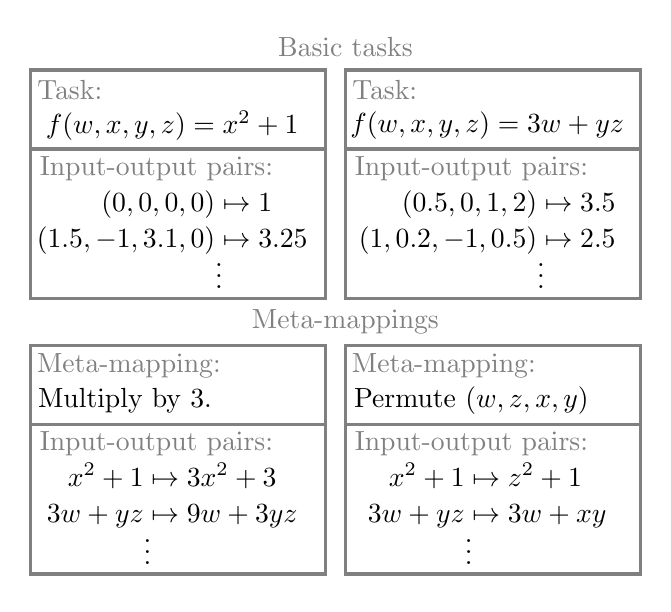
\begin{tikzpicture}[auto]
%% Basic
\node[gray] at (0, 3) {Basic tasks};
\draw[boundingbox, draw=gray, fill=white] (-4, 2.7) rectangle (-0.25, -0.2);
\draw[boundingbox, draw=gray, fill=white] (-4, 2.7) rectangle (-0.25, 1.7);
\node[gray] at (-3.5, 2.45) {Task:};
\node[align=center] at (-2.2, 2) {\(f(w,x,y,z) = x^2 + 1\)};
\node[gray] at (-2.4, 1.45) {Input-output pairs:};
\node[align=center] at (-2.2, 0.5) {%
    \(\begin{aligned}
    (0, 0, 0, 0) & \mapsto 1\\[-0.2em] 
    (1.5, -1, 3.1, 0) & \mapsto 3.25\\[-0.75em] 
    & \vdots
    \end{aligned}\)};

\begin{scope}[shift={(4, 0)}]
\draw[boundingbox, draw=gray, fill=white] (-4, 2.7) rectangle (-0.25, -0.2);
\draw[boundingbox, draw=gray, fill=white] (-4, 2.7) rectangle (-0.25, 1.7);
\node[gray] at (-3.5, 2.45) {Task:};
\node[align=center] at (-2.2, 2) {\(f(w,x,y,z) = 3w + yz\)};
\node[gray] at (-2.4, 1.45) {Input-output pairs:};
\node[align=center] at (-2.2, 0.5) {%
    \(\begin{aligned}
    (0.5, 0, 1, 2) & \mapsto 3.5\\[-0.2em] 
    (1, 0.2, -1, 0.5) & \mapsto 2.5\\[-0.75em] 
    & \vdots
    \end{aligned}\)};
\end{scope}

%% meta-mapping
\node[gray] at (0, -0.5) {Meta-mappings};

\begin{scope}[shift={(0, -3.5)}]
\draw[boundingbox, draw=gray, fill=white] (-4, 2.7) rectangle (-0.25, -0.2);
\draw[boundingbox, draw=gray, fill=white] (-4, 2.7) rectangle (-0.25, 1.7);
\node[gray] at (-2.75, 2.45) {Meta-mapping:};
\node[align=center] at (-2.8, 2) {Multiply by 3.};
\node[gray] at (-2.4, 1.45) {Input-output pairs:};
\node[align=center] at (-2.2, 0.5) {%
    \(\begin{aligned}
    x^2 + 1 & \mapsto 3x^2 + 3\\[-0.2em] 
    3w + yz & \mapsto 9w + 3yz\\[-0.75em] 
    & \vdots
    \end{aligned}\)};
\end{scope}

\begin{scope}[shift={(4, -3.5)}]
\draw[boundingbox, draw=gray, fill=white] (-4, 2.7) rectangle (-0.25, -0.2);
\draw[boundingbox, draw=gray, fill=white] (-4, 2.7) rectangle (-0.25, 1.7);
\node[gray] at (-2.75, 2.45) {Meta-mapping:};
\node[align=center] at (-2.4, 2) {Permute \((w, z, x, y)\)};
\node[gray] at (-2.4, 1.45) {Input-output pairs:};
\node[align=center] at (-2.2, 0.5) {%
    \(\begin{aligned}
    x^2 + 1 & \mapsto z^2 + 1\\[-0.2em] 
    3w + yz & \mapsto 3w + xy\\[-0.75em] 
    & \vdots
    \end{aligned}\)};
\end{scope}
\end{tikzpicture}
\caption[The polynomial task domain.]{The polynomial task domain. A basic polynomial task consists of regressing a single polynomial, i.e. the inputs are points in \(\mathbb{R}^4\) and the outputs are the value of the polynomial at that point. These basic regression tasks can be transformed by various meta-mappings, such as multiplying by a constant, or permuting their variables. }\label{fig:HoMM_polynomials:tasks}
\end{figure}

\begin{figure}[htbp]
\centering
\includegraphics[width=0.5\textwidth]{2-HoMM/figures/polynomials_adaptation.png}
\caption[Meta-mapping results in the polynomials domain.]{Meta-mapping results in the polynomials domain. We plot zero-shot performance (normalized, see text) on new tasks via meta-mappings. The system not only-generalizes trained meta-mappings to examples it has never seen before (purple), but also generalizes to held-out meta-mappings from examples (orange), and does both substantially better than a baseline model which does not adapt (dotted lines). Thus our approach is able to flexibly adapt to a new polynomial without any data from that polynomial, based on that polynomial's relationship to polynomials it has experienced.}\label{fig:HoMM_polynomials:results}
\end{figure}

\begin{figure}[htbp]
\centering
\includegraphics[width=0.625\textwidth]{2-HoMM/figures/polynomials_adaptation_by_mapping.png}
\caption[Meta-mapping results in the polynomial domain, broken down by meta-mapping type.]{Meta-mapping results in the polynomials domain, broken down by meta-mapping type. We plot a normalized performance measure, as in Fig. \ref{fig:HoMM_polynomials:results}. The system is performing well across all meta-mapping types, although there is some variability. Triangles show performance of a baseline model that does not adapt --- note that this baseline performs decently on some meta-mappings, while in other cases such a model results in worse performance than outputting all zeros.} \label{fig:HoMM_polynomials:results_by_mapping}
\end{figure}

As a proof of concept, we first demonstrate the success of our approach in polynomial regression (see Fig. \ref{fig:HoMM_polynomials:tasks}). Specifically, we construct basic tasks that consist of regressing polynomial functions (of degree \(\leq 2\)) in four variables (i.e. from \(\mathbb{R}^4 \rightarrow \mathbb{R}\)). We sampled these polynomials by first uniformly sampling a subset of variables to be included, and then sampling coefficients from \(\mathcal{N}(0, 2.5)\) for the possible monomials. These basic tasks can be inferred from (input, output) tuples, where the input is a point in \(\mathbb{R}^4\) and the output is the evaluation of that polynomial at that point. (We actually restrict the input range to \([-1, 1]\) to avoid testing extreme outlier points.) This is a simple meta-learning regression problem. 

These tasks/polynomials can then be transformed by various meta-mappings --- we considered squaring a polynomial, permuting its variables, or adding or multiplying by a constant. We trained the model on 100 basic polynomials, and we train mapped versions of 60 of these for each meta-mapping. We can evaluate the performance of that meta-mapping on the remaining 40 target tasks (corresponding to the 40 other basic polynomials) that the model has never experienced before. We also held out some of these meta-mappings to evaluate the ability of our method to generalize at the meta-mapping level (see above). For example, we can train the model to adapt to a subset of the input variable permutations, and then evaluate its ability to adapt to a held-out permutation based on examples of that permutation. In total, we trained on 20 meta-mappings, and held-out 16, corresponding to 2260 (\(=100 + 60 \times 36 \)) trained basic tasks, and 1440 held-out for evaluation. 

\textbf{Training:} We trained the system in epochs, during which it received one training step on each trained basic task and one training step on each trained meta-mapping, interleaved in a random order. For one step of training on a basic task, we used 1024 evaluations of the polynomial --- we present the model with 50 example evaluations from which to generate a task representation, and make one gradient update that improves the predictions on the remaining evaluations (as well as the example ones). This encourages the model to generate an accurate representation of the polynomial from seeing a (relatively) small set of evaluations. 

For one step of meta-mapping training, we take task representations for each of the 60 basic tasks (and corresponding target tasks) on which the meta-mapping is trained, where each basic task representation is computed from 50 examples as above. We randomly chose half of these (input task, output task) pairs to provide as examples of the meta-mapping from which to generate a representation, and train the system to match the output embeddings from the meta-mapping to the targets for all 60 examples. This encourages the model to generate a representation of the meta-mapping from half the available examples that will generalize to the other half.

To evaluate the system on a trained meta-mapping, we parameterize the mapping using all 60 input-output function embedding pairs that were used to train the meta-mapping, and evaluate the performance resulting from applying that mapping to the other 40 basic tasks to perform their 40 corresponding held-out target tasks. The system never experienced those 40 target tasks during training. Similarly, to evaluate on a held-out meta-mapping, we use 60 (input task, output task) pairs where both the input and target basic tasks were trained, and evaluate on 40 trained input tasks for which the corresponding 40 targets have not been trained. However, in the case of a held-out meta-mapping, the meta-mapping itself is never encountered during training. This ensures that the system is able to infer a new meta-mapping based on basic tasks that it has experienced, mapped in a way it has not experienced. 

Furthermore, when evaluating a meta-mapping (either trained or held-out), we do not simply evaluate how closely the output embeddings match the targets. Instead, we use each of those output embeddings to perform the appropriate task --- i.e. we use a dataset of 1024 polynomial evaluations to compute the MSE between the predictions produced by the model with the mapped embedding, and the true target polynomial. See the Supplemental Information for futher details on training and evaluation.

\subsubsection{Results}
In Fig. \ref{fig:HoMM_polynomials:results}, we show the success of our meta-mapping approach in this setting. We plot a normalized performance measure, which is 0\% if the system outputs all zeros for every polynomial, and 100\% if the system performs perfectly. Specifically, we measure performance as \(1 - \text{loss}/c\), where \(c\) is the loss for a baseline model that always outputs zero.\footnote{This measure is closely related to the variance explained, except that the square meta-mapping skews the mean of the output polynomials slightly away from zero.} We also show performance of a baseline model which just performs the original tasks without adaptation (dotted lines). Our HoMM approach is able to achieve 89.0\% performance (bootstrap 95\%-CI across runs [88.3, 89.8]) on a polynomial it has never experienced during training, based on a trained meta-mapping, and 85.5\% performance (bootstrap 95\% CI [85.1, 85.9]) based on a held-out meta-mapping. By comparison, not adapting would yield only 4.3\% and 19.3\% performance, respectively. That is, our system is able to achieve good performance on a new task without any data, based only on its relationship to prior tasks. It is able to do so much better than a baseline model which does not adapt to the new tasks. 

To further explore this performance, in Fig. \ref{fig:HoMM_polynomials:results_by_mapping} we plot the results for each of the different meta-mappings we considered: adding a constant, multiplying by a constant, permuting the variables, and squaring the polynomial. Some of these mappings are more challenging than others, as can be seen from the performance of a baseline model that does not adapt (dotted lines). For example, adding a constant to a polynomial does not alter it too drastically, so the non-adapting baseline performs well there. By contrast, multiplying by a constant sometimes changes the sign of the polynomial, so the non-adapting baseline performs extremely poorly there. The HoMM approach results in good performance across all the types of meta-mappings we considered, although unsurpsingly performance is slightly better on the easier tasks, and generalization to the held-out permutation meta-mappings is more challenging than generalization to e.g. the held-out addition ones. 

\textbf{Representation analysis:} In order to explore the performance of the model further, we performed principal components analysis on the task and meta-mapping representations in the HoMM model after training (Fig. \ref{fig:HoMM_polynomials:reps_overall_PCA}). This analysis reveals strikingly similar organization of the representation space across different training runs, with constant polynomials pushed to the outside in a semi-circle, and more complex polynomials stretching toward the center, where meta-mappings and meta-classifications are located. This may be due to the learning dynamics --- the distance of the task representations from the center appears to be roughly inversely proportional to the complexity of the task, which might imply that the constant polynomials have the largest-magnitude representations because they are easiest to learn. 

To analyze this further, in Fig. \ref{fig:HoMM_polynomials:reps_const_poly_PCA} we plot the representations for only the constant polynomials, colored by their value (square-root compressed for clarity). This shows that the constant polynomials are consistently arrayed angularly from lowest to highest value.

Finally, we examined the meta-mapping representations more closely (Fig. \ref{fig:HoMM_polynomials:reps_meta_mapping_PCA}). This analysis shows that the mappings have a consistent organization across runs, with permutations and addition grouping tightly, but multiplication and squaring, which more drastically alter the polynomials, more dispersed. In particular, multiplying by negative numbers and squaring, which can change polynomials signs and therefore cause a more drastic adaptation, are more separated from the remaining meta-mappings. It is also interesting to note that the addition meta-mappings appear to be organized more by absolute value than sign in at least some runs. 

\begin{figure}[ptbh]
\centering
\includegraphics[width=\textwidth]{2-HoMM/figures/polynomial_reps/overall_PCA.png}
\caption[Principal components of task and meta-mapping representations of HoMM after training on the polynomials domain.]{Principal components of task and meta-mapping representations of HoMM after training on the polynomials domain. The representation space is organized relatively consistently across runs, with constant polynomials pushed to the outside, and meta-mappings and meta-classifications more centrally located.} \label{fig:HoMM_polynomials:reps_overall_PCA}
\end{figure}

\begin{figure}[ptbh]
\centering
\includegraphics[width=\textwidth]{2-HoMM/figures/polynomial_reps/constant_poly_PCA.png}
\caption[Principal components of constant polynomial representations, showing systematic organization by value.]{Principal components of constant polynomial representations, showing systematic organization by value. Intriguingingly, this relationship appears to be systematically non-linear across runs. (PCs computed across all task representations, color scale of values is compressed with a square-root transformation.)} \label{fig:HoMM_polynomials:reps_const_poly_PCA}
\end{figure}

\begin{figure}[ptbh]
\centering
\includegraphics[width=\textwidth]{2-HoMM/figures/polynomial_reps/meta_mapping_PCA.png}
\caption[Principal components of meta-mapping representations in the polynomial domain, showing systematic organization by type.]{Principal components of meta-mapping representations in the polynomial domain, showing systematic organization by type. Permutation mappings cluster tightly, as do addition, while multiplication and squaring are more dispersed. The addition and multiplication mappings are partially organized by absolute value.} \label{fig:HoMM_polynomials:reps_meta_mapping_PCA}
\end{figure}

\subsubsection{Inadequacy of vector analogies for meta-mapping} \label{sec:HoMM:vector_analogies_inadequate}

One possible implementation of meta-mapping would be to just construct an analogy vector and use that for the mapping. This is motivated by work showing that word vector representations often support vector analogical reasoning; for example if we denote the vector for the word king as \(\vec{v}_{king}\), relationships like \(\vec{v}_{queen} \approx \vec{v}_{king} + \left(\vec{v}_{man} - \vec{v}_{woman} \right)\) often hold \citep{Mikolov2013}. Thus, adopting a similar strategy for meta-mapping would be superficially plausible. For example, in the polynomials domain, the meta-mapping ``Permute \((w, z, x, y)\)'' could be estimated by taking the vector differences between the representations of inputs and targets, computing an average difference vector, and adding that to the held-out examples to produce an output for each one.

However, in this section, we prove that such an approach cannot accurately represent all the meta-mappings in the polynomials domain. Furthermore, we sketch a proof by construction that our linear task network (i.e. an affine transformation, matrix multiplication plus a bias vector) parameterized independently for each meta-mapping suffices.

\textbf{Proof that vector analogies are inadequate:} In essence, the proof is simply that many of our meta-mappings are non-commutative, while vector addition is commutative. Consider the mappings for adding 1 to a polynomial, and multiplying by 2. Assume there were vector representations for these mappings, respectively \(\vec{m}_{+1}\) and \(\vec{m}_{\times 2}\). Let \(\vec{f}_{x}\) be the vector representation for the polynomial \(f(w,x,y,z) = x\). Then \(\vec{f}_{x} + \vec{m}_{+1} = \vec{f}_{x+1}\), \(\vec{f}_{x} + \vec{m}_{\times 2} = \vec{f}_{2x}\). But then:
\[ \vec{f}_{2(x + 1)} = \left(\vec{f}_{x} + \vec{m}_{+1}\right) + \vec{m}_{\times 2} = \vec{f}_{x} + \vec{m}_{+1} + \vec{m}_{\times 2} = \left(\vec{f}_{x} + \vec{m}_{\times 2}\right) + \vec{m}_{+1} = \vec{f}_{2x + 1}\]
Thus such a representation would result in contradictions, such as \(2x + 1 = 2x + 2\). Similar issues occur for permutation and other non-commutative mappings.

\textbf{Proof sketch that affine transformations in an appropriate vector space suffice:} Suppose that we have a vector representation for the polynomials, where there is a basis dimension corresponding to each monomial, so that the polynomial can be represented as a vector of its coefficients. (This is the standard vector-space representation for polynomials.) Then permutation corresponds to permuting these monomials, i.e. a permutation of the basis dimensions, which is a linear transformation. Adding a constant corresponds to adding to one dimension, which requires only the vector addition part of the affine transformation. Multiplying by a constant requires multiplying each dimension, i.e. a block-diagonal linear transformation.

Squaring polynomials is slightly more complex, and requires augmenting the vector space with components whose values are the product of the coefficients of each pair of monomials. In this case, squaring corresponds to a simple linear transformation. However, this augmentation makes the other meta-mappings more complex. The most difficult case is adding a constant, which requires shifting each pair term containing a constant by the product of the constant and the coefficient of the other monomial, but this again reduces to simply an appropriately parameterized affine transformation --- each pair term containing a constant term simply needs the added constant as a weight times the component for the other monomial. Thus affine transformations suffice in this setting.

Of course, with a sufficiently complex, deep, recurrent, and non-linear task network, any meta-mapping could be computed in principle, since a sufficiently complex network is Turing-complete \citep{Siegelman1992}. Thus, our approach to meta-mapping is fully general, conditioned on a sufficiently complex task network, while simpler approaches may not be.



\subsection{Aside: HoMM \& cognitive control}
\begin{figure}
\centering
\includegraphics[width=0.5\textwidth]{2-HoMM/figures/stroop_results.png}
\caption[Measuring the default behavior of the HoMM architecture on a Stroop-like task.]{Measuring the default behavior of the HoMM architecture on a Stroop-like task. We plot the bias of the model towards word or color responses, when given an all-zeros task representation, at different proportions of training on words or colors, and different stages of training. When the model has just mastered the less frequent task, it exhibits a default bias towards the more frequent task. However, later in training, when it has mastered both tasks, it exhibits a paradoxical bias towards the \emph{less} frequent task.} \label{supp_fig:HoMM_cognitive_control}
\end{figure}

Although it is not the primary focus of this project, the HoMM architecture could be of interest to researchers in cognitive control, even beyond the idea of meta-mapping as adaptation. The architecture offers an instantiation of a model which can perform different tasks based on task examples or language inputs, which is fundamentally the same problems human face when we must adapt our behavior. There are a number of features of the model that offer the opportunity for intriguing investigations based on this idea. For example, the task network in our architecture has a default set of bias weights that are modulated by the HyperNetwork. These can be thought of as the ``automatic'' or ``default'' processing habits of the system, whereas the weight alterations the HyperNetwork imposes can be thought of as the exertion of cognitive control to modulate behavior. 

To explore this, we trained our architecture on a very simple stroop task taken from \citet{Cohen1990}. The model receives two sets of two inputs, that can be thought of as corresponding to ``word'' and ``color'' domains. One input in each domain is turned on, representing a color word written in a color. The model's task is to report either the color or the word, depending on context.

The context we give the model is in the form of examples of the task as (input, output) pairs as usual. These are used to construct a task representation, which is then used to modulate the parameters in the task network, via a HyperNetwork.\footnote{For this experiment, we used similar hyperparameters to the polynomials experiments, except we used a much smaller model --- a single-layer task network, a $Z$-dimensionality of 8, and $\mathcal{H}, \mathcal{M}$ had 64 hidden units per layer. We optimized the model via stochastic gradient descent with a learning rate of \(0.01\) to follow more closely the approach taken by Cohen et al., although results are similar with other optimizers.} We trained the model repeatedly with different proportions of training on the word task vs. the color task, in order to investigate the default vs. controlled behavior in different training regimes. Specifically, we compared training the model to the point that it barely mastered the less frequent task (when it first achieves 100\% performance and cross-entropy loss \(< 0.3\) on both tasks) to the point that it had mastered both tasks (100\% performance and cross-entropy loss \(<0.01\) on both). We then tested the model's default behavior by giving it an all-zeros task representation, and seeing whether its performance was more aligned with the ``word'' or ``color'' task.

In Fig. \ref{supp_fig:HoMM_cognitive_control}, we show the results. We plot the bias as \(2 \times (\text{word accuracy} - \text{color accuracy})\), which is \(-1\) if the model is responding only to color, 1 if the model is responding perfectly to word, and 0 if it is responding equally to each (or otherwise responding randomly). When the model has just barely mastered the less-frequent task, it exhibits a default bias towards the more frequent task. However, once we train it to full master of both tasks, it exhibits a surprising paradoxical bias towards the task that was mastered more recently. This may relate to observations that switching from a less-practiced task back to a more practiced one is difficult \citep{Monsell2003}, possibly because performing the less-practiced task requires strong suppression of the default behavior. It's possible that in the course of achieving full mastery on the less-practiced task, the more practiced task must be so suppressed that it fades away from being the default. These phenomena provide possible inspiration for future investigations in cognitive control.


\section{Discussion}\label{sec:HoMM:discussion}

We have proposed meta-mappings as a computational account of the human ability to perform a novel task zero-shot (without any data), based on the relationship between the novel task and prior tasks. We have shown that our homiconic meta-mapping architecture performs well in a proof-of-concept polynomial regression setting. Here, we will briefly discuss some of the work in machine learning and cognitive science that inspired this project. We will discuss the broader implications of our work and future directions in more detail in Chapter \ref{chapter:conclusions}. 

\subsection{Related work in machine learning}
As mentioned above, there is a large body of prior work on zero-shot learning based on natural-language descriptions of tasks. \citet{Larochelle2008} considered the general problem of behaving in accordance with language instructions as simply asking a model to adapt its response when conditioned on different ``instruction'' inputs. Later work explored zero-shot classification based on only a natural language description of the target class \citep{Socher2013,Romera-Paredes2015,Xian2018}, or of a novel task in a language-conditioned RL system \citep{Hermann2017, Hill2019a}. Some of this work has even exploited relationships between tasks as a learning signal \citep{Oh2017a}. Other work has considered how similarity between tasks can be useful for generating representations for a new task \citep{Pal2019}, but without transforming task representations to do so. Furthermore, similarity is less specific than an input-output mapping, since it does not specify \emph{along which dimensions} two tasks are similar. To my knowledge none of the prior work has proposed using meta-mapping-like approaches to adapt to new tasks by transforming task representations, nor has the prior work proposed a parsimonious homoiconic model which can perform these mappings.

This work is also related to the rapidly-growing literature on meta-learning \citep[e.g.][]{Vinyals2016, Santoro2016, Finn2017a, Finn2018, Stadie2018, Botvinick2019, Ravichandran2019}. Our architecture builds directly off of prior work on HyperNetworks \citep{Ha2016} and other recent applications thereof  \citep[e.g.][]{Brock2018a, Zhang2019, Li2019a, Rusu2019}. In particular, recent work in natural language processing has shown that having contextually generated parameters can allow for zero-shot task performance, assuming that a good representation for the novel task is given \citep{Platanios2017} -- in their work this representation was evident from the factorial structure of translating between many pairs of languages. Our work is also related to the longer history of work on different time-scales of weight adaptation \citep{Hinton1982, Kumaran2016} that has more recently been applied to meta-learning contexts \citep[e.g.][]{Ba2016, Munkhdalai2017, Garnelo2018} and continual learning \citep[e.g.]{Hu2019}. It is more abstractly related to work on learning to propose architectures \citep[e.g.][]{Zoph2016, Cao2019}, and to models that learn to select and compose skills to apply to new tasks \citep[e.g.][]{Andreas, Andreas2016, Tessler2016, Reed2015, Chang2019a}. In particular, some of the work in domains like visual question answering has explicitly explored the idea of building a classifier conditioned on a question \citep{Andreas, Andreasa}, which is related to our approach in the visual categorization tasks (Chapter \ref{sec:extending:concepts}).

Work in model-based reinforcement learning has also partly addressed how to transfer knowledge between different reward functions \citep[e.g.][]{Laroche2017}; the HoMM approach is more general. For example, rather than needing a new reward function to be given, meta-mapping provides a principled way to infer a new reward estimator by transforming a prior one. Meta-mapping could also be used to transform a transition function used in the planning model in response to environmental changes. Our insights could therefore complement model-based approaches, which provides an exciting direction for future work.

There has also been other recent interest in task (or function) embeddings. Achille et al. \citep{Achille2019} recently proposed computing embeddings for visual tasks from the Fisher information of the parameters in a model partly tuned on the task. They show that this captures some interesting properties of the tasks, including some types of semantic relationships, and can help identify models that can perform well on a task. Rusu and colleagues recently suggested a similar meta-learning framework where latent codes are computed for a task which can be decoded to a distribution over parameters \citep{Rusu2019}. Other recent work has tried to learn representations for skills \citep[e.g.][]{Eysenbach2019} or tasks \citep[e.g.]{Hsu2019} for exploration and representation learning, but has not explored transforming these representations to achieve zero-shot performance on a novel task.

In summary, our perspective builds on several lines of prior work in machine learning. While there has been substantial prior work on meta-learning, task representation, and there have even been other approaches to zero-shot task performance, to the best of our knowledge none of the prior work has explored zero-shot performance of a task via meta-mappings. In the following chapters, we will show experimentally that this approach yields better performance than alternative approaches across a variety of domains. We suggest that it may complement other approaches to adaptibility, such as model-based RL.

\subsection{Related work in cognitive science}
Our model is inspired by several streams of research in cognitive science as well. We will briefly review some of these here, in order to provide some grounding for the rest of the dissertation. However, we will discuss most of these issues in greater detail in Chapter \ref{chapter:conclusions}, when we reflect on the dissertation as a whole.   

A first inspiration is a long line of research has suggested that analogical transfer between structurally isomorphic domains may be a key component of ``what makes us smart'' \citep{Gentner2003}. Analogical transfer has been demonstrated across various cognitive domains \citep[e.g.][]{Bourne1970, Day2011}. Yet there has been relatively little exploration of adaptation without any examples of the new task at all. 

This dissertation also touches on the issues of compositionality and systematicity. Some researchers have advocated that cognition must rely on strictly compositional representations in order to exhibit systematic and productive generalization \citep[e.g.][]{Fodor2001,Lake2017}.  We avoided explicitly enforcing compositional task representations in our model, instead allowing those representations to emerge. This has several advantages. First, it requires much less hand-engineering for each application domain (e.g. our model did not need the notion of variables or permutation built into it to generalize to held-out permutation meta-mappings), and second, it may allow for novel decompositions at test time. (See Chapter \ref{chapter:conclusions} for further discussion.) 

Some aspects of the HoMM architecture may also seem reminiscent of the modularity of mind for which Fodor advocated \citep{Fodor1983modularity}, particularly the fact that we divided the model into feed-forward input and output systems, with the flexible, task-specific computations in the middle shared across many domains. In fact, we believe that perception and task-processing are mutually constraining and reinforcing, but for simplicity our model does not incorporate all aspects of this. Cognitive modeling always requires some simplification in order to provide a useful description of the system. (Again, see Chapter \ref{chapter:conclusions} for further discussion.)   

Finally, as we showed above, the HoMM architecture and approach may related to areas like cognitive control. Similarly, our shared workspace for data points, tasks, and meta-mappings relates to ideas like the Global Workspace Theory of consciousness. Exploring these connections would be an exciting direction for future work. 

In summary, meta-mapping and the HoMM architecture draw inspiration from many areas of research in cognitive science. I hope that this work will reciprocally provide inspiration to many researchers in this field. In support of this, the subsequent chapters explore our model on a variety of tasks more relevant to human cognition, and make direct comparisons to the adaptation abiilites of humans and language-conditioned models. 


\chapter{Comparing to human adaptation} \label{chapter:human}

In the previous chapter we proposed a framework for modeling human adaptation to new tasks, based on relationships between tasks. To understand whether we have developed a good model, it is necessary to compare its adaptation to human adaptation. It is worth stopping for a moment to consider how flexible humans actually are. We certainly experience short-term interference from switching tasks or goals \citep{Rogers1995}, or when we try to override a habitual response \citep{Stroop1935, MacLeod1991}. Over longer periods of time, our adaptation might be a response to learning in the new situation, rather than the type of zero-shot flexbiility that HoMM is intended to model. How flexibly are humans able to adapt to task changes in a short amount of time? \par
Unfortunately a complete evaluation of human flexibility is a large research program. In this chapter we evaluate human adaptation in one setting, inspired by those used as demonstrations in the previous chapter. In particular, we implemented a more human-comprehensible version of the poker-like card game we used for those experiments, and evaluate how well participants are able to switch to losing the game, after learning to win it. \par

\section{Experimental design}
We made several changes to the game used in the previous experiments to make it easier for humans to learn. We changed the rules to follow a more hierarchical structure, and we made it so no money was gained or lost on ties. \par
The game we had participants play was a simplified variation of poker. They were dealt hands which consisted of two cards, each with a number (rank) between 1 and 4, and a color (suit) of red or black. The participants played against a computer opponent that was dealt a similar hand. The hands were ranked such that straight flushes (adjacent cards in the same suit) beat adjacent cards in a different suit, which beat non-adjacent cards (including pairs). Ties were broken by the highest card, or by suit if both cards were tied. \par
\begin{figure}
\centering
\begin{subfigure}[b]{0.5\textwidth}
\includegraphics[width=\textwidth]{3-human-adaptation/figures/pre_bet_screenshot.png}
\caption{Before betting.}
\end{subfigure}%
\begin{subfigure}[b]{0.5\textwidth}
\includegraphics[width=\textwidth]{3-human-adaptation/figures/post_bet_screenshot.png}
\caption{Feedback.} \label{fig:human_betting_trial_feedback}
\end{subfigure}%
\caption{The card game experiment trials, as seen by participants.} \label{fig:human_betting_trial}
\end{figure}
On each trial, participants were dealt a hand and asked to make a bet of 0, 5, or 10 cents (see fig. \ref{fig:human_betting_trial}). If their hand beat the opponent's hand, they won the bet amount. If their hand lost, they lost it. If the hands were tied, they neither won nor lost money. \par
The experiment had several phases. First, participants were instructed in the rules and payment scheme for the experiment. Next, they were instructed on the rules of the game. After this, they were tested with four hand-comparison trials intended to probe their understanding of each of the rules of the game. If they failed more than one of these trials, they were not allowed to continue with the experiment. \par
Following this understanding check, subjects played a block of 32 hands (sampled to have a diversity of expected values), where they saw the results of their play, as in (fig. \ref{fig:human_betting_trial_feedback}). After this block, they played a similar block of 24 trials where they did not see the results of their play. The results were replaced with a brief grayed-out screen, and participants were payed the net expected value of their actions over the block (rounded to the nearest 10). This provides an evaluation phase with relatively less potential for learning. \par
Finally, participants were told that we wanted them to try to lose for the remaining trials, and that ``for the remainder of the experiment, if you bet and lose, you’ll gain the amount you bet, and if you bet and win, you’ll lose the amount you bet.''. They were then given an attention check to evaluate whether they had understood this instruction. Subjects who failed this attention check were excluded from the analysis. They then played another block of 24 trials where they were rewarded for losing instead of winning (i.e. the expected returns were reversed). As in the previous block, they did not see the results of their actions. They were finally asked a few demographic questions. See Appendix \ref{appendix:human} for detailed instructions \& methods.\par
Our main target comparison was performance in the two blocks without feedback -- were participants able to switch their behavior to lose at the game as well as they won at it?\par


\section{Human performance}
First, how well were participants able to learn the game? Participants performance is reasonable, although they are far from optimal, and there is substantial individual variability (fig. \ref{fig:human_cards_basic_results}). In particular, participants are sometimes making intermediate bets, which an optimal agent would never do. Furthermore, all subjects thresholds (where they cross a betting probability of 0.5) are variable, some subjects are substantially over- or under-conservative. However, performance is actually more optimal than some basic statistics might suggest, see Appendix \ref{appendix:human:suboptimality}. \par 
Participants also performed above chance, but far from optimally after being asked to lose (fig. \ref{fig:human_cards_losing_results}). So how well were they able to adapt? 

\begin{figure}
\centering
\begin{subfigure}[t]{0.5\textwidth}
\includegraphics[width=\textwidth]{3-human-adaptation/figures/testing_basic_bet_densities.png}
\caption{Bet density by expected value.}
\end{subfigure}%
\begin{subfigure}[t]{0.5\textwidth}
\includegraphics[width=\textwidth]{3-human-adaptation/figures/testing_basic_subject_response_fits.png}
\caption{Probability of non-zero bet by expected value. The red dashed line is the optimal threshold, the grey curves are the individual subject fits.}
\end{subfigure}%
\caption{Card game behavior, basic game evaluation block. While participants are performing well above chance, they are far from optimal. They make intermediate value bets, and do not switch optimally between betting and not betting. There is also substantial inter-subject variability.} \label{fig:human_cards_basic_results}
\end{figure}
\begin{figure}
\centering
\begin{subfigure}[t]{0.5\textwidth}
\includegraphics[width=\textwidth]{3-human-adaptation/figures/testing_losing_bet_densities.png}
\caption{Bet density by expected value.}
\end{subfigure}%
\begin{subfigure}[t]{0.5\textwidth}
\includegraphics[width=\textwidth]{3-human-adaptation/figures/testing_losing_subject_response_fits.png}
\caption{Probability of non-zero bet by expected value. The red dashed line is the optimal threshold, the grey curves are the individual subject fits.}
\end{subfigure}%
\caption{Card game behavior, losing block. There is again substantial inter-subject variability.} \label{fig:human_cards_losing_results}
\end{figure}


\section{Adaptation in humans and HoMM}
Human adaptation was quite good, in the sense that on average performance was almost identically preserved (fig. \ref{fig:human_cards_adaptation_results}). However, this average masks substantial individual variability. Because the figure plots \emph{expected} earnings, and hand values were closely matched, almost all the change from one point to the next is due to either stochasticity in the participants policies, or non-standard adaptation. (We cannot call this non-standard adaptation sub-optimal, since it sometimes results in \emph{improved} performance on the adapted task.) It would be interesting to explore in detail what factors underlie this variability, but here we focus on the comparison to the HoMM model, and generalization to a language-based model which receives task names. \par  
\begin{figure}
\centering
\includegraphics[width=0.8\textwidth]{3-human-adaptation/figures/human_adaptation.png}
\caption{Human adaptation in the cards experiment: the change in performance from the winning evaluation block to the losing evaluation block. Larger lines are the average, smaller are individual subjects. While there is substantial individual variability, average performance is preserved.} \label{fig:human_cards_adaptation_results}
\end{figure}
In order to perform the task with the HoMM model, we had to make one minor alteration. Because the model only receives feedback on the action it took, this is not a simple regression problem with inputs and targets. It is more similar to a reinforcement learning setting, where the model takes actions and may or may not receive rewards in response (although there is no temporal component in our simplified tasks). We thus altered the way a task representation is constructed from examples in the model. Instead of using a dataset of (input, target) tuples, we used a dataset of (input, (action, reward)) tuples, where the action and reward were processed together to form a single embedding. The model was then trained with a masked loss, such that it only updated its predictions for actions it actually took, rather than other possibilities. The language-based model was altered similarly. \par
In Fig. \ref{fig:human_cards_homm_results} we plot the adaptation of the models against the human results. Both models are performing near-optimally on the training tasks, but of course they have much more experience with these tasks than the humans do. However, the adaptation of the models is substantially different. Both models are worse at the losing versions of the tasks, but the HoMM model is only slightly worse, while the language-based model is degrading to near chance performance. \par
In order to make a more fair comparison between humans and the models, in Fig. \ref{fig_humans_cards_homm_change_scores} we plot performance on the losing task, as a percentage of performance on the winning tasks. Note, however, that this metric is biased against the models, because of the ceiling effect -- their scores on the adapted tasks cannot be higher than their optimal scores on the original tasks, whereas the humans are only optimal on average because many of them are performing substantially better on the adapted tasks, for unclear reasons. While HoMM is adapting slightly sub-optimally, the difference between it and the human subjects is not statistically significant, either by a \(t\)-test (\(t(18.54) = -1.80\), \(p = 0.09\)), or a permutation test (\(p > 0.05\)). However, HoMM is significantly better than the language-based approach, either by a   \(t\)-test (\(t(5.37) = 9.33\), \(p < 0.001\)), or a permutation test (\(p < 0.005\). \par

\begin{figure}
\centering
\includegraphics[width=0.8\textwidth]{3-human-adaptation/figures/human_adaptation_vs_HoMM.png}
\caption{Comparing human adaptation to the HoMM and language models.}\label{fig:human_cards_homm_results}
\end{figure}

\begin{figure}
\centering
\includegraphics[width=0.8\textwidth]{3-human-adaptation/figures/change_scores.png}
\caption{Comparing adaptation (as \% of score on prior task) between humans and the models. While the HoMM model is slightly sub-optimal, it is not significantly different than humans. By contrast, the language-based model is near chance on the held-out tasks.} \label{fig:human_cards_homm_change_scores}
\end{figure}

\section{Discussion}

\chapter{Extending meta-mapping to more complex tasks} \label{chapter:extending}
In the previous chapters we have demonstrated the succes of meta-mapping in two simple domains. While these have allowed us to demonstrate the efficacy of the approach relative to other baselines, and compare its adaptation to that of humans, there are several reasons to extend beyond these to more complex tasks. \par 
First, the approach relies on several pieces which it is not obvious would scale to more complex settings, such as representing an entire task with a single vector, parameterizing the task network via a HyperNetwork conditioned on this vector, and learning meta-mappings from relatively few task examples. If any of these fails to extend to more complex settings, it could limit the applications of our approach. \par
Second, there are limitations to toy experiments. While toy experiments can provide carefully controlled demonstrations of an idea, we have shown in other work that more systematic generalization can emerge when agents are placed in more realistic settings \citep{Hill2019a}. This may impact both the meta-mapping approach and the language baseline, so it is important to evaluate the effects of richer environments on both. This will help inform us as to whether our approach will be useful in more complex settings. (Unfortunately, creating truly realistic environments and training agents in them requires complex implementations and substantial computational resources. Thus, in this chapter we demonstrate our results in environments of moderate complexity, and leave the extension to even richer environments to future work.)\par 
To address these motivations, in this chapter we present experiments on extending our ideas to two important settings: reinforcement learning and classification from raw pixel inputs. These settings are important both because they are dominant paradigms for applying deep learning, and because they have deep connections to cognitive modelling \citep[e.g.][]{Yamins2014, Kriegeskorte2015, Momennejad2017}. \par

\section{Reinforcement learning}

Reinforcement learning is an interesting (and challenging) application for meta-mapping for several reasons. First, reinforcement learning has deep roots in neuroscience, and appears to relate to some computations in the brain \citep{Sutton2017, Niv2009, Odoherty2003, Dabney2020}. Second, reinforcement learning has achieved impressive human-level performance on complex tasks such as Atari games \citep{Mnih2015}, Go \citep{Silver2016, Silver2017}, and complex video games like Dota 2 \citep{OpenAI2019}, and Starcraft II \citep{Vinyals2019}. This motivates it as an important place to explore more human-like intelligence. Third, there has been a rich vein of research on adaptation in reinforcement learning from language-conditioned models \citep{Hermann2017} to the observation that model-based methods or successor representations can allow for adaptation to environment changes \citep{Daw2014, Momennejad2017}. However, these latter methods assume that a new reward function is given, which requires a substantial portion of the adaptation problem already be solved. Thus, there is substantial room to ask whether meta-mapping can provide good performance in RL tasks, and good motivation for a language baseline. \par 
\subsection{Tasks}
To address these challenges we created a set of RL tasks based on raw visual input with a relatively simple action space. Refer to Fig. \ref{fig:extending_grid_task_views} throughout this section for images of the visual input the agent would receive. The tasks take place in a \(6 \times 6\) room with an additional impassable barrier of \(1\) square on each side. The squares are upsampled at a resolution of 7 pixels per square to provide the raw visual input to the agent. In addition, the agent receives egocentric input, since we have shown in other work that this is beneficial to generalization \citep{Hill2019a}. That is, the agent's view is always centered on itself, and the world moves around it as the agent moves. The agent has four actions available to it, corresponding to moving in the four cardinal directions. If it makes an invalid action, such as trying to move past the edge of the board, the state does not change. The view window is sufficiently larger than the world so that the agent can see the entire world, no matter where it is.\par 
The tasks the agent must perform relate to objects which are placed in this space. The objects can appear in 10 different colors. In any given task, the world will have two colors of objects in it. Each color of objects only appears with one other color, so there are in total 5 possible colors that can appear. In any given task, one of the present colors is ``good,'' and the other is ``bad.'' On some tasks, the good and bad colors in a pair are switched.\par
There are two types of tasks, a ``pick-up'' task, and a ``push-off'' task. The tasks are visually distinguishable to the agent, because the shape of the objects used for them are different. In the pick-up task, the agent is rewarded for picking up the good-colored objects by moving to their grid locations, and is negatively rewarded for picking up the bad-colored objects. In the push-off task, the agent is able to push an adjacent object by moving toward it, if there is no other object behind it. The agent is rewarded for pushing the good-colored objects off the edges of the board, and negatively rewarded for pushing the bad colored objects off. The two types of tasks (``pick-up'' and ``push-off'') are visually distinguishable to the agent, because the shape of the objects used for them are different. However, which color is good or bad is not visually discernable, and must be inferred from the example (state, (action, reward)) tuples used to construct the task representation.\par 
There are in total 2 task types \(\times\) 5 color pairs \(\times\) binary whether the good and bad colors are switched \(= 20\) tasks in total. We trained the system on 18 of these, holding out the switched color combination of (``red'', ``blue'') in both task types. That is, during training the agent always is positively rewarded for interacting with red objects and negative rewarded for interacting with blue objects across both task types. We train the system on the ``switch-good-and-bad-colors'' meta-mapping using the remaining three color pairs in the two task types, and then evaluate its ability to perform the held-out tasks zero-shot based on this mapping. Note that this is a quite difficult challenge for a model-free system, since any rewards it receives during training on similar-colored tasks are the opposite of these evaluation rewards.\par
\begin{figure}[!htb]
\centering
\begin{tikzpicture}[auto]%, scale=0.8, every node/.style={scale=0.8}]
\draw[boundingbox, draw=gray, fill=white] (-9.3, 2.65) rectangle (0.3, -2.3);
\node[gray, align=center] at (-4.6, 2.35) {Pick-up task};
\node at (-7, 0) (pu1) {\includegraphics[width=4cm]{4-extending/figures/grid_tasks/pick_up_3.png}};
\node at (-2, 0) (pu2) {\includegraphics[width=4cm]{4-extending/figures/grid_tasks/pick_up_4.png}};
\node at (-4.5, 0) {\huge \(\bm \downarrow\)};
%\draw[arrow, very thick, gray] (pu1) -- node[black] {\huge``\(\bm \downarrow\)''} (pu2);

\begin{scope}[shift={(0, -5.5)}]
\draw[boundingbox, draw=gray, fill=white] (-9.3, 2.65) rectangle (0.3, -2.3);
\node[gray, align=center] at (-4.6, 2.35) {Push-off task};
\node at (-7, 0) (pu1) {\includegraphics[width=4cm]{4-extending/figures/grid_tasks/pusher_9.png}};
\node at (-2, 0) (pu2) {\includegraphics[width=4cm]{4-extending/figures/grid_tasks/pusher_10.png}};
\node at (-4.5, 0) {\huge \(\bm \leftarrow\)};
%\draw[arrow, very thick, gray] (pu1) -- node[black] {\huge``\(\bm \downarrow\)''} (pu2);
\end{scope}
\end{tikzpicture}
\caption[Illustrative state transitions from the RL grid experiments.]{Illustrative state, action, state transitions from the RL grid experiments. In the pick-up task example (top), the agent moves downward and picks up the green object. In the push-off task example (bottom), the agent moves left and pushes the red object. Views are the visual input the agent would receive. The agent is the white triangle, note that it is always at the center of the view, because of the egocentric perspective.} \label{fig:extending_grid_task_views}
\end{figure}

\subsection{Model}
%% TODO: detailed parameters
To accomodate this setting, we essentially combined the DQN architecture \citep{Mnih2015} with our previous approaches. That is, the input to the model was raw pixels, which were passed through several convolutional layers to produce state embeddings. This visual processing was shared across all tasks. As in the card game tasks discussed in previous chapters, we used (state, action, reward) tuples as input to the meta-network \(\mathcal{M}\). More precisely, we processed actions and rewards through several layers to produce an ``action-outcome'' embedding, and then concatenated that to the visual embedding as input to \(\mathcal{M}\). As before, \(\mathcal{M}\) produced a task embedding, which was passed through a HyperNetwork \(\mathcal{H}\) to parameterize the task network \(F\). The task network took state embeddings output by the convolutional network, and processed these to produce to produce output embeddings, which were linearly decoded to Q-values for the different actions. When meta-mapping, the input task embeddings replaced the input state embeddings to \(\mathcal{M}\) and \(F\), and the output task embeddings replaced the action-outcome inputs to \(\mathcal{M}\). See Appendix \ref{app:extending_grids_methods} for further details of the architecture and training. \par 
Perhaps because of the difficulty of the generalization problem in this setting, we found that two additional model modifications were useful. First, rather than constructing the task embedding completely from scratch each time, we kept persistent task embeddings cached, and used a random convex-combination of the output of \(\mathcal{M}\) and the cached embedding to perform the task. We added an additional \(\ell_2\) loss between the cached and transient embedding that attempted to match each to the other. Having partially persistent embeddings made it easier for the system to overcome the initial confusion about the fact that objects were sometimes positively rewarding and sometimes negatively rewarding, and made it easier for it to discover the overall structure of the tasks. \par
Second, we found that incorporating weight normalization \citep{Salimans2016} in the task network increased the stability of the training process. In the simpler settings of the cards tasks, neither of these modifications was necessary. It is likely that the temporally extended nature of these tasks makes the interference between the conflicting tasks worse. However, it is possible that with appropriate hyperparameters, and enough training and time, the model could overcome this and learn without persistent representations or weight normalization in this setting as well. \par 

\subsection{Results}

\begin{figure}
\centering
\begin{subfigure}{0.5\textwidth}
\includegraphics[width=\textwidth]{4-extending/figures/grids_adaptation_results.png}
\caption{Adaptation performance at best-validation epochs.}\label{fig:HoMM_RL_results:accuracy}
\end{subfigure}%
\begin{subfigure}{0.5\textwidth}
\includegraphics[width=\textwidth]{4-extending/figures/grids_adaptation_correlation_loose.png}
\caption{Correlation of performance on the two tasks.}\label{fig:HoMM_RL_results:correlation}
\end{subfigure}%

\caption[Results on the RL tasks.]{Results on the RL tasks. (\subref{fig:HoMM_RL_results:accuracy}) Performance on the held-out tasks via a meta-mapping and via language generalization. Despite the challenging nature of the adaptation (as evidenced by the language-generalization performance), HoMM is performing quite well. (\subref{fig:HoMM_RL_results:correlation}) Correlation of performance on the two hold-out tasks, across runs and time points where performance on the training tasks is high. The correlation is much stronger in the HoMM model than in the language-generalization model, that is, the HoMM model is behaving more systematically in the sense that it is generalizing similarly on both tasks. (Results from 5 runs, error-bars in panel \subref{fig:HoMM_RL_results:accuracy} are bootstrap 95\%-CIs across runs.)} \label{fig:HoMM_RL_results}
\end{figure}

\begin{figure}
\centering
\includegraphics[width=0.5\textwidth]{4-extending/figures/grids_language_learning_curves.png}
\caption[Language generalization model learning curves on the RL tasks.]{Average performance of the language generalization model over training on the RL tasks. The model exhibits intriguing but transient generalization early in learning, before it has understood the full structure of the tasks (especially the more difficult and sequential push-off task). However, this quickly decays to below-chance generalization as the model masters the training tasks. This early generalization is not included in the main results since the train accuracy at this time is below the threshold of having adequately learned the tasks.} \label{fig:HoMM_RL_language_learning_curves}
\end{figure}

In Fig. \ref{fig:HoMM_RL_results} we show the results. We optimally stop the model for each task by requiring the training accuracy to be above a threshold (95\% for the HoMM model, but 87.5\% for the language model, because stricter thresholds resulted in worse language results), and using the other task as a validation set --- that is, we evaluate the model on one task when the model performs well on the other task as well as the training tasks. The HoMM model substantially outperforms the language model, achieving 88.0\% of optimal rewards (mean, bootstrap 95\%-CI [75.0-99.0]) on the held-out pick-up task, and 71.7\% (mean, bootstrap 95\%-CI [42.0, 94.6]) on the held-out push-off task. By contrast, the language model is showing very little adaptation, with respective performance of -92.8\% (mean, bootstrap 95\%-CI [-96.3, -88.4]) and -79.7\% (mean, bootstrap 95\%-CI [-92.8, -59.1]) on the two tasks. This difference between the models is significant in a mixed linear regression controlling for task type and a random effect of run (\(t (20.6) = -19.515\), \(p < 1\cdot10^{-14}\)).\footnote{Degrees of freedom calculated by the Satterthwaite approximation.}\par

The HoMM model also exhibits significantly stronger correlations between its performance on the two tasks, both within runs at different time-points and across runs (Fig. \ref{fig:HoMM_RL_results:correlation}, Supp. Fig. \ref{fig:app_extending:RL_correlation_by_run}). Specifically, the HoMM model has a correlation of \(r=0.82\) between performance on the two tasks, while the language model only has a correlation \(r=0.10\), and this difference is significant in a mixed linear model predicting push-off performance from pick-up performance, controlling for task type, epoch, and the random effect of run (main effect of HoMM \(t(451.3) = 4.76\), \(p < 1\cdot 10^{-5}\), interaction of HoMM with pick-up performance \(t(452.0) = 3.43\), \(p < 1 \cdot 10^{-3}\)). At a surface level, this means that it is easier to select a good stopping point for the HoMM model --- even though the language model is achieving less bad (though still at or below chance) performance at some points in some runs, the lack of correlation between the results on the different tasks means there is no fair way to stop training the model at that point. More fundamentally, this suggests that the meta-mapping approach is exhibiting more systematic generalization, in the sense that it is either generalizing well on both tasks, or not generalizing well on both. Again, this is more like what would be expected from human cognition.

Intriguingly, the language model does transiently exhibit slightly positive generalization very early in learning (Fig. \ref{fig:HoMM_RL_language_learning_curves}) --- however, as the model beings to master the training tasks, the generalization quickly decays to substantially below chance. The early generalization is not included in the main results in Fig. \ref{fig:HoMM_RL_results} because the train set performance is below even the more generous threshold we set for the language model. Even if it were included, this early performance is significantly worse than the HoMM model's results. \par



\section{Concepts}

There is a long history of cognitive research on how people learn concepts or categories \citep{Bourne1970, Medin1978, Kruschke1992, Goodman2008}. This work has focused almost entirely on how people can learn a concept from examples, and more recent work in the area has focused on areas like active learning by choosing the examples to test \citep{Markant2014, Markant2015}. However, humans can also understand concepts without any examples at all. If I teach you that ``blickets'' are red triangles by examples, and then I tell you that ``zipfs are blue blickets,'' you will instantly be able to recognize a zipf without ever having seen an example (Fig. \ref{fig:extending_concept_example}). This type of zero-shot performance can be understood as applying a ``switch-red-to-blue'' meta-mapping to the ``blicket'' classification function. This motivates applying our approach to the domain of concepts. \par 

\subsection{Tasks}
%% TODO: detailed methods, rework this figure
\begin{figure}
\centering
\begin{tikzpicture}[auto]%, scale=0.8, every node/.style={scale=0.8}]
% blickets
\node at (-4.8, 2.2) {\LARGE ``Blickets''};
\draw[decoration={calligraphic brace, amplitude=0.5cm},decorate,line width=1mm] (-3, 0.3) -- (-3, 4);
\node at (-2, 3.1) {\includegraphics[width=1.8cm]{4-extending/figures/categorization_stimuli/32_red_triangle_0.png}};
\node at (-2, 1.2) {\includegraphics[width=1.8cm]{4-extending/figures/categorization_stimuli/24_red_triangle_0.png}};

% not blickets
\node at (-5.2, -2.1) {\LARGE ``Not blickets''};
\draw[decoration={calligraphic brace, amplitude=0.5cm},decorate,line width=1mm] (-3, -4) -- (-3, -0.3);
\node at (-2, -3.1) {\includegraphics[width=1.8cm]{4-extending/figures/categorization_stimuli/32_red_circle_0.png}};
\node at (-2, -1.2) {\includegraphics[width=1.8cm]{4-extending/figures/categorization_stimuli/24_yellow_triangle_0.png}};
\node at (3, 3.5) {\LARGE ``Zipfs = blue blickets''};
\node at (1.6, 0) {\LARGE ``Zipfs?''};
\draw[decoration={calligraphic brace, amplitude=0.5cm},decorate,line width=1mm] (3.2, -2.9) -- (3.2, 2.9);
\node at (4.2, 1.9) {\includegraphics[width=1.8cm]{4-extending/figures/categorization_stimuli/24_red_triangle_1.png}};
\node at (4.2, 0) {\includegraphics[width=1.8cm]{4-extending/figures/categorization_stimuli/32_blue_triangle_1.png}};
\node at (4.2, -1.9) {\includegraphics[width=1.8cm]{4-extending/figures/categorization_stimuli/32_blue_inverseplus_1.png}};
\end{tikzpicture}
\caption[An example of zero-shot visual concept understanding that can be captured by a meta-mapping.]{An example of zero-shot visual concept understanding that can be captured by a meta-mapping. We can understand what zipfs are if we learn about blickets, and about how zipfs relate to blickets.} \label{fig:extending_concept_example}

\end{figure}

We constructed stimuli by selecting from 8 shapes (triangle, square, plus, circle, a t shape, an outline of a square, an outline of a triangle, and 4 small squares forming a larger square) and 8 colors (red, green, blue, yellow, purple, pink, cyan, and ocean). We rendered these stimuli at 3 sizes (16, 24, and 32 pixels) at a random position and rotation within a \(50 \times 50\) pixel image, to produce stimuli like those shown in figure \ref{fig:extending_concept_example}. See Appendix \ref{app:extending_categorization_methods} for renderings of each shape, color, and size. \par
We defined the basic task mappings as binary classifications of the images (i.e. functions from images to \(\{0, 1\}\)). We gave the system all the uni-dimensional concepts as training examples of concepts (i.e. one-vs-all classification of each shape, color, and size), so that it would be able to recognize all the basic attributes. We also constructed a set of composite tasks based on conjuctions, disjunctions, and exclusive-disjunctions (XOR) of these basic attributes. For each concept, we chose the examples so that the datasets were balanced (that is, there was an 50\% chance that each item in the dataset was a member of the category), both during training and evaluation. We only included negative examples that were one change away from being a member of the category. These careful contrasts may be beneficial during training -- recent work has shown contrasting examples to be useful for causing neural networks to extract more general concepts \citep{Hill2019}. They also make the evaluation more challenging, and increase the ability to dscriminate partial understanding of the concept from complete understanding. We trained the system on a subset of the concepts, and on meta-mappings that switched one shape for another, or switched one color for another. We evaluated the system on its ability to apply these meta-mappings to basic tasks it was trained on in order to perform the held-out basic tasks. Because there are many meta-mappings available in this setting, we were able to hold out one shape meta-mapping and one color meta-mapping for evaluation, and we will also show results on adaptation based on these held-out mappings. \par  

\subsection{Model}
We used a 4-layer convolutional network for input embedding, and a linear task network \(F\) (although for the language comparison we used a 3-hidden-layer network, which resulted in improved performance in that condition). We found that constructing task representations from language was more effective here than constructing them from examples. \par
We also found that in this setting the optimal architectures for the task network differed for language-based generalization and meta-mapping-based generalization. In particular, we show in Appendix \ref{app:extending_categorization_lang_arch} that, while a linear task network worked better for the meta-mapping model, a nonlinear and deeper one generalized better from language. This is likely because the linear map provides a useful inductive bias for meta-mapping. This raises the possibility that adding linear skip-connections to nonlinear task networks which might allow for better meta-mapping performance as well as better task representations. It is also possible that using examples and language together to infer tasks would improve task representations further. Both of these provide exciting directions for future investigations. \par 

\subsection{Results}

We found that constructing task representations from language worked better than construting task representations from examples in this setting. In Fig. \ref{fig:extending_concepts_adaptation}, we show that language generalization (mean \(= 0.92\), bootstrap 95\%-CI \([0.89, 0.94]\)) appears better than that obtained from meta-mapping task representations constructed from examples (mean \(= 0.90\), bootstrap 95\%-CI \([0.89, 0.91]\)). However, this comparison is not statistically significant under a mixed model (\(t(8) = -1.5\), \(p = 0.18\)). However, meta-mapping with language-based task representations performs better (mean \(= 0.95\), bootstrap 95\%-CI \([0.94, 0.97]\), mixed-model \(t(8) = -2.9\), \(p = 0.02\)). Thus it appears that language may be a better way of constructing task representations in this setting, but meta-mapping a prior task still results in better zero-shot generalization than language alone. \par

\begin{figure}
\centering
\includegraphics[width=0.8\textwidth]{4-extending/figures/concepts_adaptation.png}
\caption[Accuracy on held-out visual concepts.]{Accuracy on held-out visual concepts based on meta-mapping (either from examples or language), or language generalization. While language generalization appears non-significantly better than meta-mapping from examples, transforming language-based task representations with meta-mapping performs significantly better.} \label{fig:extending_concepts_adaptation} 
\end{figure}

Why does language result in better task representations in this setting? Of course, language conveys the basic concept more cleanly than examples can, but this was also true in other settings where language did not seem as advantageous. While we cannot completely answer this question, we note several points. First, we gave the system substantially more training tasks here than in the prior settings, and this larger amount of data may be necessary to keep the language system from overfitting. Second, several exciting lines of work are converging on the role of language in shaping our concept representations. Recent work has shown that more ``nameable'' concepts are easier to understand \citep{Lupyan2020}, and that language may be beneficial to visual concept learning in machine learning \citep{Mu2019}. Thus, these results may be reflective of broader issues about how concepts are formed. \par

\section{Discussion}


\chapter{Learning across different timescales} \label{chapter:timescales}

%% TODO: probably mention SWIL somewhere in these first few paragraphs
A large amount of recent machine learning research can be seen as studying interactions of learning across different time-scales. In particular, the field of meta-learning is based on the idea that a model can slowly learn over many experiences how to learn rapidly in a new experience. Similarly, the previous chapters show how slowly-accumulated knowledge about tasks and their relationships can allow zero-shot inferences about a new task. \par 

However, both of these approaches examine how slowly learned knowledge can improve rapid learning. Yet one of the core motivations of complementary learning systems theory was that rapidly learned experiences could be integrated into our prior knowledge. There is a lack of research investigating how what we learn over short time scales, for example in the inner loop of a meta-learning algorithm, can be integrated with our longer term knowledge. \par 

Integration of knowledge in machine learning is mostly studied under the continual learning. Most work on continual learning investigates the setting where a model, starting from \emph{tabular rasa}, must learn a sequence of tasks without forgetting \citep{Ven2018, Atkinson2018}. This is motivated by the clear ability of humans and animals to learn multiple tasks without forgetting. However, humans are not starting from a blank slate when they achieve this. Indeed, \citep{Velez2017} show that systems can meta-learn to learn without forgetting. This raises the possibility that works that examine continual learning from a blank slate are misleading, because prior learning can be an important part of the solution. \par 

We have shown in the prior chapters that using knowledge of prior tasks can allow the system to perform well on a new, related task without any data. Here, we highlight the impacts of this perspective on different time-scales of learning. In particular, we first show that this zero-shot inference improves learning on the new task, and second, that the knowledge encoded in the system can allow this learning to occur without even the possibility of interference with prior tasks. \par  

\section{Starting points for learning}

When humans arrive at a novel task, we often receive some instructions as a starting point. These instructions often describe the relationship of the novel task to prior experiences. This observation served as the motivation for the previous chapters, in which we showed that using meta-mapping could improve zero-shot task performance. However, as soon as we start performing a task, it is no longer zero-shot. That is, zero-shot adaptation is most important insofar as it serves as a useful starting point for later learning. In this chapter, one of our primary goals is to compare the zero-shot ``guess'' at a task representation to other initializations of the task representation, to evaluate whether it is a beneficial starting point for learning. \par 
In order to do this, we use an approach related to our prior work on one-shot learning of word embeddings \citep{Lampinen2018a}. In that work, we integrated a novel word into a pre-trained language model by simply optimizing its embedding(s) to improve the model's prediction of it in context. We showed that this allowed reasonable learning of new words, in fact average performance with this method was not statistically different than if the word had been included in the training corpus from the beginning. Thus in a model that has been pre-trained to understand the latent structure of a system (such as language), optimizing the representation of a single object can often be sufficient to construct a high-quality representation of the object, without needing to alter the other parameters of the model. \par
%% TODO: SWIL here as well.
Analogously, in this chapter we explore optimizing the task embedding of a novel task once the system has begun to perform it. We will show that optimizing the task embedding alone will often allow near-perfect performance on a novel task, provided the model that is pre-trained on sufficiently many other tasks from the same distribution. This means that a new task can be learned without the possibility of any interference with prior tasks, because only task-specific parameters are altered. This provides a new perspective on continual learning (though see \citep{Oswald2020} for some related observations). Rather than thinking about how a system can minimize interference when learning a sequence of tasks from \emph{tabula rasa}, we should perhaps ask how prior knowledge can allow learning without any interference at all. \par 
The important observation from our perspective is that a zero-shot guess at a task embedding provides a useful starting point for this optimization. In particular, we compare to a variety of other initializations, and show that the zero-shot guess provides faster learning, and lower cumulative error. This latter measure can be thought of as analogous to the notion of \emph{regret} in reinforcement learning, a measure of how sub-optimally the algorithm performs while learning to behave optimally. Starting from the output of a meta-mapping results in learning faster, and making fewer mistakes along the way. This may be part of the solution to why humans are able to learn faster and more accurately than deep learning models on novel tasks. \par   

\section{The polynomials domain}

%% TODO: add updated results and baseline in untrained model 
We begin by demonstrating these results in the simple polynomial regression domain that we considered in chapter \ref{chapter:zero_shot_via_homm}. We compare three different initializations. First, a small random initialization, as is often used for parameters of a deep model prior to training. Second, initializing each task with the embedding of a random trained task, in case the distributions of these is helpful for later learning. Finally, we compare to the guess embedding produced by meta-mapping from a prior task. \par 
As noted above, we make this comparison by optimizing the task embeddings for the new tasks. We do this without altering any other parameters in the model. It is not clear that this would be sufficient to produce good performance on a novel task, indeed we show below that in an untrained model it is not. However, if the model has sufficient experience of related tasks, it does suffice. \par 
We used a similar distribution of tasks to our polynomial results presented above, except that we ensured every evaluation task was a trained meta-mapping of a trained task, but where that task had not been used as an example for the meta-mapping during training. This eliminates the uncertainty introduced by having to learn a new task or mapping from examples, as well as applying the transformation, which allows for a more controlled comparison. To be precise, we trained the system on 60 base tasks plus the results of applying 20 meta-mappings to them. We additionally trained the system on 40 new base tasks, and held out the results of applying the 20 meta-mappings to them. It is these \(40 \times 20 = 800\) novel tasks that we optimized the embeddings for. \par 


\chapter{Conclusions \& looking ahead} \label{chapter:conclusions}

Despite the recent success of deep learning, it still lacks some of the features of human intelligence. In this dissertation, I have focused on how humans are able to reuse our knowledge flexibly in new tasks, before we have any data on those tasks. I have suggested that a computational mechanism underlying this is an ability to transform prior task representations to adapt them to a new task. I have proposed meta-mapping -- higher-order tasks that transform task representations -- as a computational model of this type of adaptation. \par
In order to evaluate this idea, I have provided a parsimonious implementation of the meta-mapping framework in the form of Homoiconic Meta-Mapping (HoMM) architectures. I have demonstrated the effectiveness of HoMM by showing its zero-shot task performance across a wide variety of domains, from polynomial regression to visual classification and reinforcement learning. HoMM is often able to achieve 80-90\% performance on a new task with no data on that task at all. This brings deep learning models a step closer to human-like flexibility. This work therefore has implications for both cognitive science and artificial intelligence. In this chapter I will review these contributions, and their broader implications. \par  

\section{Contributions}

I have proposed meta-mappings as a computational account of the human ability to perform a novel task zero-shot (without any data), based on the relationship between the novel task and prior tasks. The fundamental idea is that tasks should be performed from a task representation, and that adaptation can be implemented as a transformation of a task representation. Thus adaptation can be interpreted as a meta-mapping, a higher-order task that maps between representations of more basic tasks. \par  

To instantiate this idea, I have proposed HoMM architectures. These architectures embed data points, tasks, and meta-mappings into a shared representational space, and use shared systems to infer and execute transformations of that space. That is, the same systems are used regardless of the entities (data, tasks, etc.) over which a computation is being executed. Sharing the representational space and transformation systems is parsimonious --- it does not multiply networks unnecessarily. Furthermore, I see this proposal as a logical development from the fundamental idea of meta-learning: that tasks themselves can be seen as data points in a higher-order task. This leads to the reciprocal idea of transforming task representations just like we manipulate data, i.e. a \emph{homoiconic} approach. \par  

I have shown that meta-mapping, as implemented in the HoMM architecture, performs well across a wide range of settings. The computational paradigms I considered range from regression to classification to reinforcement learning, with inputs ranging from simple multi-hot vectors to images. Across these settings, HoMM often achieves 80-90\% performance on a new task without data from that task, based on the relationship between the new task and a prior task. When given enough experience with the task space, as in the visual classification settings with enough training tasks, it is able to achieve perfect adaptation. In many runs (though not all), it is even able to do so with held-out meta-mappings. \par

\textbf{Language generalization:} I compared HoMM to the standard paradigm of zero-shot learning --- constructing a task representation from natural language \citep[e.g.][also see below]{Larochelle2008}. While language-based generalization can be effective, our HoMM approach is generally more sample efficient at generalizing to tasks far outside its training experience, at least in the settings we considered. That is, HoMM needs fewer training tasks to generalize well zero-shot. While the language model performs comparably at interpolating to closely related tasks, as in the visual concepts domain, HoMM appears to offer stronger extrapolation to tasks farther from those on which it has been trained. This effect is demonstrated clearly when the new tasks directly contradict prior tasks, as in the card games and RL domains.\par

Furthermore, HoMM seems to exhibit more systematic generalization than the language-conditioned models. For example, HoMM resulted in more runs with perfect generalization at moderate-sample sizes in the visual concept tasks, while the language generalization results were more graded. HoMM also exhibited more strongly correlated performance on the held-out RL tasks --- when it was performing well on one of the tasks, it was performing well on the other. This is more like the systematic behavior that humans often exhibit. \par

\textbf{Some notes of caution:} However, these results should not be interpreted as suggesting that language is not important or useful. Instead, language and meta-mapping should be seen as complementary. They may be applicable in different domains, and could potentially be mutually supporting. Cognition is complex, and any single model is guaranteed to be an oversimplified approximation of human cognitive processes in real-world situations. Indeed, an interesting future direction would be to consider how meta-mapping and language can mutually constrain one another when adapting to a new situation. I am not claiming that meta-mapping is the only cognitive mechanism for adaptation. Instead, my results demonstrate that meta-mapping may be useful as one tool for building models with more human-like adaptibility.  \par

\textbf{Adaptation as a starting point:} I would also like to highlight the results showing that meta-mapping provides a useful starting point for later learning. While meta-learning approaches often construct a good starting point for learning any task from the known distribution, they do not use task relationships to offer a uniquely valuable starting point for each novel task. My results show that starting from adapting a prior task can substantially reduce the errors made along the way to mastering the new task. The efficiency of human learning may be partly explained by adaptation before beginning the task. \par 

\textbf{Summary:} HoMM provides a model of a possible computational mechanism underlying cognitive adaptibility, and the role that adaptibility may play in future learning. Language likely plays an important role as well, and future work should explore uniting these approaches. 

\section{On flexibility in natural and artificial intelligence}

In the introduction, I noted how researchers in cognitive science have aggressively critiqued deep learning for its lack of flexibility \citep[e.g.][]{Lake2015, Lake2016, Lake2017, Marcus2018}. We have addressed one challenging aspect of flexibility in this work -- the ability to take our knowledge of a task, and adapt to some variation. While this might be challenging for standard deep-learning models, the general framework of meta-mapping makes it possible. Thus, at their most basic level, these results present a challenge for those who would say deep-learning models are too inflexible to be accurate cognitive models. \par  
Indeed, I see my project as following in the tradition of work that explores how systematic, structured generalization can emerge from the structure of learning experience, without needing to be built into the model itself \citep{McClelland2010a, McClelland2010, Hansen2017}. This is a challenge to arguments that cognition must rely on strictly compositional representations in order to exhibit systematic and productive generalization \citep[e.g.][]{Fodor2001, Fodor2008lot2, Lake2017}. Without building in compositional representations of tasks, our model can learn to exploit the shared structure in the concept of ``losing'' across a few card games to achieve 85\% performance in losing a game it has never tried to lose before. \par 

There are a number of potential benefits to letting the compositional structure emerge. First, the structure does not need to be hand-engineered specially for each domain. Our system required no special knowledge about the domains beyond the basic tasks and the relationships between them. The fact that some of these relationships corresponded to e.g. permutations of variables in the polynomial domain did not need to be hard-coded, instead the model was able to discover it from the patterns of the mappings (presumably, since it was able to generalize well to held-out permutations). The second advantage of letting compositionality emerge is that it can potentially allow for novel decompositions at test time. The ability of our model to perform well on held-out meta-mappings supports this hope, but further work will be needed to verify it. \par

In summary, I suggest that meta-mapping offers a way to create models that can bring deep learning systems closer to the flexibile intelligence of the human mind. While I have demonstrated these results in some simple settings, one of the powerful features of deep learning is that its results tend to improve as datasets grow more complex and realistic \citep{Hill2019a,Radford2019,Sutton2019}. I hope that this research will help guide the way to building even more flexible models in more realistic domains.  \par

\section{Relating to cognitive science}

Our work provides a tool for modeling human adaptibility, which has many potential direct applications. It offers an explanation for how humans might be able to adapt when told ``watch out, the floor is slippery,'' or recognize a pink-and-green striped car even if they have never seen one before, by transforming their task representations. This is a fundamental aspect of human intelligence, but is often omitted from cognitive models. However, our work has broader relevance as well. \par 

\textbf{Fast and slow transfer:} In Chapter \ref{chapter:introduction}, I reviewed the cognitive science and machine learning literatures from a Complementary Learning Systems perspective. In particular, I sugested that humans' slow learning of shared structure in the world can itself provide transfer benefits, but also helps set up the representations necessary for faster transfer mechanisms. This idea is reflected in the organization of the HoMM architecture. A great deal of perceptual and action processing is shared across tasks (though see below), so that the model can exploit the shared visual features of different games or objects. The representations constructed by these shared systems are used for both task inference and for task performance. This allows the system to perform a novel task from a few examples (as in standard meta-learning), or based solely on its relationship to prior tasks, by meta-mapping. The fast zero-shot transfer achieved by meta-mapping thus relies on the representations of tasks and data that are constructed over the full development of the network. \par

Furthermore, this fast transfer ability itself must be learned over time. However, once it has been learned, it can then generalize to new examples and even new meta-mappings. This reflects my suggestion that humans not only learn good representations for fast transfer, but actively practice the act of adaptation. I hope my work will inspire broader thought about how different systems of transfer, operating over different timescales, can support each other in order to achieve the flexibility of human intelligence.\par

\textbf{Abstraction \& recursion:} Abstraction \& recursion offer one exciting area where our model could potentially offer a new modeling framework. It would be interesting to explore how concepts can be recursively built upon other concepts, as happens in learning of mathematics \citep{Wilensky1991, Hazzan1999, Lampinen2017b}. For example, addition can be seen as repeated succession, multiplication can be seen as repeated addition, exponentiation as repeated multiplication, and this process is recursively continued in up-arrow notation. A homoiconic system like HoMM seems closer to being able to capture this recursive construction of concepts. It would be interesting to explore how our architectures could model this type of recursive construction of concepts. \par 

Relatedly, I believe that my model moves closer to capturing some of the recursive processing that Jerry Fodor and others have considered to be important \citep[e.g.][]{Fodor2008lot2}. I have drawn particular inspiration from ideas about how humans re-represent their knowledge into more generalizable forms \citep{Karmiloff-Smith1986,Clark1993}. As a reminder, that work examines fascinating developmental trajectories where, even after initial behavioral mastery of some concept is achieved, various implicit and explicit measures of understanding continue to evolve. It would be interesting to explore whether auxiliary learning objectives over task representations and meta-mappings, and the shaping effects of language (see below), could model some of these phenomena. Could the change in behavior on a particular task be driven by the evolution of its task representation while learning a meta-mapping involving that task? Could unsupervised learning over task representations make clusters and structure within the space of tasks salient, thereby regularizing and structuring behavior? Exploring these questions will be an exciting direction for future work. \par 

\textbf{Consciousness:} I have also been inspired by computational models of how conscious knowledge may be built on top of implicit knowledge \citep{Cleeremans2014}, as well as by the Global Workspace Theory \citep{Baars2005}. HoMM's shared representational space for data points, tasks, and meta-mappings can be seen as a global workspace, over which task-specific computations can be executed. Indeed, the HoMM architecture could potentially shed light on issues about explicit vs. implicit knowledge --- it is plausible to assume that a task representation captures what we know about a task, while implicit knowledge could be captured both by the task representation and elsewhere (such as in the default weights of the task network). Exploring these ideas further could provide an exciting direction for future work. \par

\textbf{Modularity vs. generality:} The issues above also relate to ideas Fodor expressed about the modular structure of the mind, for example the view of mental processes as ``transforming internal representations'' and that what is accessible about the stimulus is only ``what is given in [...] its \emph{proximal} representations'' \citep[][pp. 200-201]{fodor1975language}. Indeed, the division of the HoMM architecture into input and output systems, with flexible, task-specific computations in the middle may seem very reminiscient of the type of modularity that he sometimes advocated \citep{Fodor1983modularity}. HoIver, I chose this implementation as a simplifying assumption --- I believe that in reality processes such as perception are not task-independent, but involve the interaction of top-down and bottom-up constraints \citep{McClelland2014}. \par

Reciprocally, I also believe that higher-level computations are influenced and constrained by the modalities in which they are supported. This computational feature can emerge in the HoMM model, as despite the fact that different types of data and tasks are embedded in a shared latent space, the model generally learns to organize distinct types of inputs into somewhat distinct regions of this space. This means that the task-specific processing can potentially usefully exploit domain-specific features of the input, as for example humans do when they use gestures to think and learn in spatial contexts like mathematical reasoning \citep{Goldin-Meadow1999, Wakefield2018}. At the same time, the shared space can allow a graded overlap in the structure that is shared across different input domains. That is, the HoMM model is able to learn what should be shared and what should be separated, whereas approaches that build such divisions in are fundamentally more limited.\par

\textbf{Language:} I noted above that our results should not be taken as a rejection of the role of language. Instead, they suggest that meta-mapping and language could be mutually supporting. It would be interesting to explore whether combining the representations produced by the language system and meta-mapping system could result in better performance than either alone, especially if this combination were weighted by some measure of uncertainty in the estimates. Furthermore, while we considered language input only in these projects, language output (explaining behavior) plays an important role in learning, both in humans \citep{Chi1994}, and in neural networks \citep{Mu2019}. While our use of task-representation-classification in some settings may have captured some aspects of this, adding richer explanations during learning will likely be important for achieving truly human-like behavior. 

\textbf{Cognitive control:} Furthermore, although it is not my primary focus in this project, the HoMM architecture may have interesting connections to cognitive control. Even without meta-mapping, the HoMM architecture instantiates an architecture that can compute flexibly in response to task demands, provided as examples or natural language. Futhermore, the ``default'' task-network weights output by the HyperNetwork could be used to model more automatic processing, which more cognitive, task-specific processing might need to override. I showed some initial experiments related to this in Chapter \ref{chapter:zero_shot_via_homm}. Meta-mapping adds many additional directions --- for example, a failure to meta-map perfectly could capture some of the challenges of task-switching. Exploring these ideas further would also be an interesting direction for future work. \par

\textbf{Neuroscience:} Finally, a major advantage of neural network models is their ability to make predictions about neuroscience. For example, neural network models have been used to understand aspects of the neural basis for perception \citep{Yamins2016a}, semantic cognition \citep{Rogers2004}, and cognitive control \citep{Shenhav2013}. We have not engaged with this level of analysis, but doing so would be an exciting direction for future work. Our HoMM architecture offers a framework that can unify perception, task representation, control, and motor outputs, all within a single model. It would be possible to relate the different components of our model to different brain regions --- visual perception to visual cortex, higher level perceptual features to more semantic regions, the action network to motor cortex, and the meta/hyper/task networks to frontal regions associated with task representation/control/working memory. Thus, our architecture could potentially provide an integrative model spanning a wide range of brain regions, although it would likely require some modifications to account for neural data well (some of which are discussed in the limitations section below). \par 

\textbf{Summary:} I take an emergent perspective on the structure of the mind, and believe that all cognitive and perceptual processes are mutually influencing and supporting. For simplicity my model does not always fully reflect this. Furthermore, I believe my approach may be broadly useful, even to researchers with different perspectives. The functional approach relates to the ideas of Fodor and Karmiloff-Smith, the perspective on adaptation draws inspiration from prior work on analogy and transfer, and the HoMM architecture could even have interesting implications for researchers interested in cognitive control or neuroscience. I hope that researchers from many of these areas will find my work inspirational.

\section{Relating to artificial intelligence}

There are a number of potential direct applications in artificial intelligence, from building more flexible vision models to building better systems for robotics. Domains like robotics are especially interesting from the meta-mapping perspective, because exploration in real world settings is costly and must be safe \citep{Turchetta2016}, and so the substantial reduction in errors made when using meta-mapping as the starting point for learning a new task may be valuable. \par 

\textbf{Reinforcement learning:} Applying meta-mapping to different types of adaptation in RL also opens many possibilites, especially in combination with model-based methods. Meta-mapping could be used as a principled way of adapting transition functions or successor representations \citep[c.f.][]{Madarasz2019}, beyond the approach of adapting model-free reward or value estimates that we demonstrated. While adapting pure model-free RL will likely be challenging in more complex task spaces, combining meta-mapping with other insights could yield much greater flexibility. For example, meta-mapping could be used with hierarchical models where language has been used as a task or sub-task representation \citep[e.g.][]{Jiang2019}. Similarly, it could be applied in planning based models, for example using monte-carlo tree search \citep[as in e.g.][]{Silver2016, Silver2017}, but with task-representation-conditioned policy and value functions. More ambitiously, meta-mapping could be explored in models that learn to plan \citep{Guez2019} rather than having that planning hand-engineered into the architecture. Many contemporary RL frameworks could potentially be augmented with meta-mapping. \par

\textbf{Abstraction:} Many of the directions of future investigation from a cognitive perspective relate to pressing problems in artificial intelligence as well. The issue of flexible abstraction is challenging in deep learning --- while feed-forward neural networks generally construct progressively more abstract representations in higher layers, the relationships between those representations are fixed by the fixed computational pathway. The shared representational space and meta/hyper networks in our model provide a suggestion for how concepts at different levels of abstraction could be integrated and used more flexibly. This would be another important step towards human-like flexibility. \par 

\textbf{Continual learning:} Finally, the work in Chapter \ref{chapter:timescales} suggests new directions in continual learning. By off-loading much of the task-specific computation to a flexible hyper-network-based architecture, and inferring and optimizing a task representation, we can enable learning of a new task without even the possibility of interfering with prior tasks. Furthermore, we can leverage our knowledge of prior tasks to learn faster than we would have in an untrained model, or without meta-mapping. This positive transfer is very different from the standard in continual learning, which mostly focuses on stemming the bleed in accuracy caused by new tasks, even in more recent works that have also incorporated hyper networks \citep{Oswald2020}. Given the importance of learning rapidly on new tasks, without interfering with prior knowledge, this is also an exciting future direction. \par 

\textbf{Summary:} In addition to the direct applications of the meta-mapping framework in building more flexible artificial intelligence systems, it suggests many exciting future directions in reinforcement learning, abstraction, and continual learning. I hope that this project will help inspire the development of deep learning systems that can adapt and learn more like humans. \par 

\section{Limitations of the present explorations}

While I have explored HoMM in a relatively broad range of computational paradigms, I have still only explored a single family of architecture within a small subset of the computational paradigms that can be found in the literature. In this section I will outline a few limitations of the present work, and corresponding ideas for future research, but note these are simply examples of the many choices made in this project that could be explored further. \par

There are a number of architectural aspects of the approach that could be altered. For example, although we used HyperNetworks to parameterize our task network, it would also be reasonable to have a fixed task network which simply receives the task representation as an additional input. We evaluated this approach in the polynomial and RL domains, and found it did not perform as well at meta-mappings (although it performed similarly at the basic tasks). However, it might be a useful approach in some settings. We also noted in the visual categories domain that linear task networks seemed to improve meta-mapping, while nonlinear ones seemed to result in better basic task performance --- thus it might be reasonable to consider a deep, nonlinear task network, but with a linear skip-connection from beginning to end. An identity (ResNet-like) inductive bias on this linear connection might be helpful as well, so that the network would only have to learn what to change about the task representation. \par 

Furthermore, although we found that homoiconic architectures were useful, it might be that in some task domains a shared representational space with shared networks across different types of tasks is detrimental. In general, whether sharing an architecture across different tasks is beneficial depends on the data regime --- shared architectures can be a useful regularizer with small datasets, but correspondingly harmful with sufficiently large ones. Thus, the answer to this question will likely depend on the depth and breadth of the training data. One cognitively-motivated intermediate option might be to have a domain general shared-system like ours, but with additional learning of more domain-specific mappings directly from inputs to outputs, which could potentially allow for the benefits of both approaches.\par

As a more general point, cognitive processing is much more complex than our model. While we relied on simple feed-forward computations for our simple tasks, using a recurrent task network, or even a more complex architecture involving memory --- such as the Differentiable Neural Computer \citep{Graves2016} --- would likely increase the ability of the model to perform and adapt on complex tasks. This would likely be necessary to reach human-level performance in many domains.\par 

Finally, the type of flexibility we have proposed is still limited in some crucial ways. It requires exactly identifying the prior task to use as a source for the adaptation, and when that adaptation should occur (i.e. where the task boundary is). It would be more realistic to relax these assumptions. This could be achieved by combining with techniques that have been used for task-change tracking in meta-learning \citep[e.g.][]{Nagabandi2019}, but could also potentially be learned end-to-end in an appropriate model given appropriate input. There are a number of linguistic cues that humans can exploit for when they should try to adapt, and a system that experiences many such transitions might learn when adaptation is warranted. \par 


\section{Looking ahead}

The next ten years will likely bring us a great deal more clarity about how far deep learning is from achieveing human-like intelligence. As I suggested in the introduction, it may be that greater scale and complexity of our architectures and training regimes will bring forth more flexible behavior from many deep neural network models. Indeed, this is almost certainly true to some extent --- overparameterization and larger datasets both tend to improve the generalization performance of deep neural networks. If translation abilities can emerge from a word-prediction model given enough data \citep{Radford2019}, couldn't the ability to adapt emerge from simple architectures trained in complex enough environments? If so, what will the contribution of this dissertation be to our future knowledge? Will it be more than another ``bitter lesson'' demonstrating that ``building in how we think we think does not work in the long run'' \citep{Sutton2019}? \par 

From an artificial intelligence perspective, even if more flexible behavior emerges in other architectures when they are placed in richer training regimes, the architectural and training innovations I have proposed in this work may still provide useful insights that allow flexibility to emerge at more feasible data scales. Many applications of artificial intelligence (from medical diagnosis to self-driving cars) would benefit from models with greater flexibility within a family of related tasks. The perspective of building and transforming task representations may also inspire future work that leverages similar abstractions --- perhaps architectures that use task-representation and HyperNetwork-based approaches like ours will be better able to accommodate diverse sets of tasks from different domains, or will be useful for challenging new evaluations of intelligence \citep[e.g.][]{Chollet2019}. \par 

From a cognitive science perspective, my work provides a computational basis for understanding the flexibility of the human mind. Cognitive modeling is always a trade-off between capturing details of the system and phenomena, and simplifying the system to make it more comprehensible; emergent behavior is generally harder to analyze than the behavior of simpler models. Models like those I have proposed here, which offer an intermediate amount of structure, may offer a useful level of complexity that allows for flexible behavior to be learned in complex task spaces (rather than built in), while also making the representational and computational basis for that flexibility available to analysis. Our architectures may also provide a framework for instantiating neuroscientific theories of higher-level cognitive processing. \par 

Ultimately, I have presented one computational perspective on how natural and artificial intelligence could flexibly adapt to new situations. I am excited to see the new perspectives the future will bring, and I hope my work will provide some inspiration for some of them. 


%\chapter{Research roadmap} \label{RR_sec}

\section{My prior work}
In my prior work, I have explored transfer and flexibility from both computational and experimental perspectives. In this section I briefly describe some of this work which I intend to include in my dissertation. \par

\textbf{Understanding human concept learning and flexibility:} In prior work \citep{Lampinen2017b}, I explored how different presentations of mathematical concepts affect human learning and ability to generalize this learning to different or more formal tasks. This captures both how transfer/grounding from slowly-learned prior knowledge can affect rapid learning of new knowledge, and how humans are able to flexibly apply this new knowledge to new situations, and generate abstractions about it. \par 
\textbf{Exploring multi-task benefits in non-linear networks:} In another line of work, I have explored the benefits of multi-task learning from a theoretical perspective. I have analyzed empirically the evolution of the representations of a network learning multiple related tasks \citep{Lampinen2017a}, yielding a minimal example of a network which shows extraction of shared structure. In brief, while a linear network cannot exploit or represent shared structure (up to a rotation of its representation space), a nonlinearity at the output suffices to allow representation of this shared structure. \par
I have also made some (unpublished) explorations of multi-task transfer with neither shared inputs nor outputs, based on purely functional relationships. These have been in the domain of learning binary functions, and show interesting patterns of transfer based on some as-yet-difficult-to-define notion of functional similarity, whether the multi-task learning is sequential or simultaneous. This helps us to understand how multi-task transfer generalizes beyond pairs of perfectly analogous tasks. \par
\textbf{Towards a theoretical understanding of multi-task benefits in linear networks:} More recently, we have derived a fully-analytic theory of generalization dynamics in deep linear neural networks \citep{Lampinen2019}, which we apply to understanding the issue of multi-task transfer. We show that transfer is most beneficial in the regime of learning a low SNR task with well-aligned auxiliary tasks (and that this pattern is qualitatively quite similar in deep nonlinear networks). I suggest that this is precisely the regime that humans work in -- we have many auxiliary tasks that are well aligned (often by cultural or pedagogical construction), and these allow us to learn well even from small samples (which are inherently lower SNR). \par 

\section{Towards more flexible deep learning architectures} \label{eml_sec}

In this section I propose a computational framework for thinking about the relationship between slow and fast transfer. This proprosal is in the form of a deep learning architecture which I will argue captures some of the aspects of human flexibility that are still missing from most contemporary deep learning models. \par

This architecture is based on ideas from meta-learning. In particular, as noted above, the fundamental insight of meta-learning is that there is a continuum between tasks and data. I attempt to follow this premise to its logical conclusion by implementing architectures which minimize the distinction between data and tasks. At the same time, my architecture exploits different timescales of learning to allow the system to slowly accumulate knowledge about regularities among data or tasks, and rapidly adapt to new data or tasks consistent with this learned structure. \par

In particular, our system learns to map different kinds of knowledge -- data, tasks, strategies, language, etc. -- into a common representational space, and meta-learns to compute mappings over this space. This allows the system to rapidly and flexibly learn and adapt. Many of the features of human flexibility are represented under a fairly unified computational principle in this framework. For example, following instructions to perform zero-shot on a task is just a mapping from language to a behavioral strategy. Trying to alter behavior on a task, such as switching from trying to win a game to trying to lose, is a mapping from one behavioral strategy to another. Explaining behavior is a mapping from behavioral strategies to language. Our system makes all these mappings in-principle learnable. \par 

One can loosely think of the common representational space as being something like a global workspace of consciousness, and the mappings within it as being the operations that we can consciously perform. Of course, these operations are constrained by the experiences we've had and the mappings we've been required to make, so the space of conscious representation may be set up to make certain types of mappings more easily realizable than others on certain kinds of data. Nevertheless, we are in principle capable of learning an arbitrary mapping between any sets of things of which we are conscious, whereas we are not necessarily capable of learning an arbitrary mapping between features that are unconsciously represented in the brain, such as the activity of a single neuron. The features which the brain learns to consciously represent are precisely those that are useful for the computations we consciously perform. These prior expectations contribute to our flexibility within the broad bounds of learned schemas, but our difficulty with adapting to tasks which are completely unlike those we've encountered before. Our architecture attempts to imitate this combination of inherent flexiblity and learned specialization. \par  

\subsection{Implementation details}
The essential idea of the architecture is that we separate the system into two parts:
\begin{enumerate}
\item Domain specific encoders and decoders (vision, language, etc.) that map into a shared embedding space $Z$
\item A meta-learning system which:
    \begin{enumerate}
    \item Embeds tasks into the shared embedding space $Z$.
    \item Learns to perform tasks in accordance with their embeddings.
    \end{enumerate}
\end{enumerate}
The utility of having a completely shared space $Z$ in which data, language, and tasks are represented is that it allows for arbitrary mappings between these distinct types of data. In addition to basic tasks, the system could in principle learn to map language to tasks (follow instructions) or tasks to language (explaining behavior), or tasks to tasks (changing behavior). This is a step closer to the flexible reasoning humans display. \par
Without training on these mappings, of course, the system will not be able to execute them well. However, ideally if it is trained on a braod enough set of such mappings, it will be able to generalize these to new instances drawn from the same data/task distribution. For instances that fall outside its data distribution or for optimal performance it may require some retraining. This reflects the structure of human behavior -- we are able to learn rapidly when new knowledge is relateively consistent with our previous knowledge, but learning an entirely new paradigm (such as calculus for a new student) can be quite slow. \par

\begin{figure}
\centering
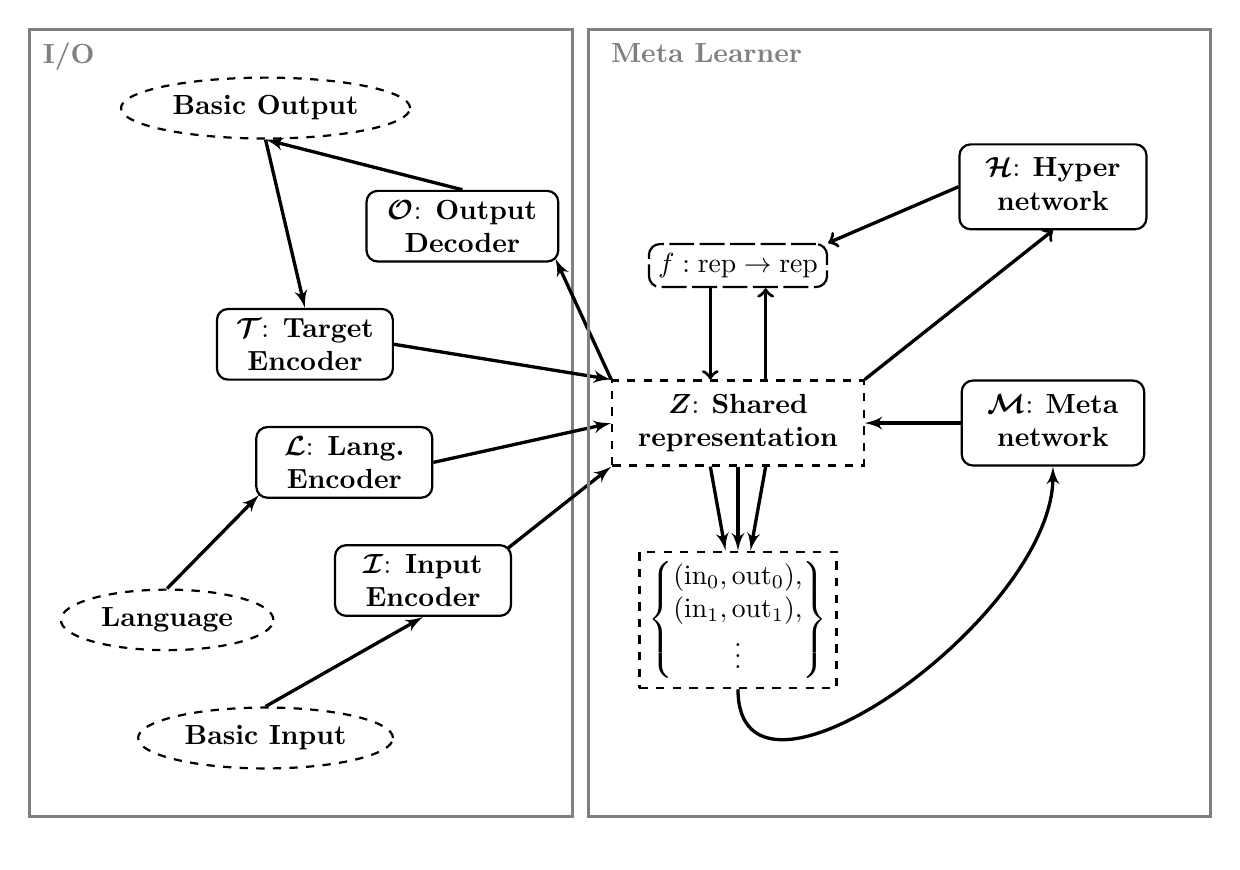
\begin{tikzpicture}[auto]

\node [dashblock] at (0, 0) (rep) {\begin{tabular}{c}$\bm{Z}$: \textbf{Shared} \\ \textbf{representation}\end{tabular}};

% inputs, outputs

\draw [boundingbox] (-9, -5) rectangle (-2.1, 5);
\node [text=gray] at (-8.5, 4.65) {\textbf{I/O}};

\node [conc] at (-6, -4) (perc) {\textbf{Basic Input}};
\node [conc] at (-7.25, -2.5) (lang) {\textbf{Language}};
\node [conc] at (-6, 4) (act) {\textbf{Basic Output}};
\node [block, text width=2cm] at (-4, -2) (IE) {$\bm{\mathcal{I}}$: \textbf{Input Encoder}};
\node [block, text width=2cm] at (-5, -0.5) (LE) {$\bm{\mathcal{L}}$: \textbf{Lang. Encoder}};
\node [block, text width=2.2cm] at (-3.5, 2.5) (OD) {$\bm{\mathcal{O}}$: \textbf{Output Decoder}};
\node [block, text width=2cm] at (-5.5, 1) (TE) {$\bm{\mathcal{T}}$: \textbf{Target Encoder}};
\path [line] (perc.north) to (IE.south);
\path [line] (lang.north) to ([xshift=0.05cm, yshift=0.05cm]LE.south west);
\path [line] ([xshift=-0.05cm, yshift=-0.05cm]IE.north east) to (rep.south west);
\path [line] (LE.east) to (rep.west);
\path [line] (rep.north west) to ([xshift=-0.05cm, yshift=0.05cm]OD.south east);
\path [line] (OD.north) to (act.south);
\path [line] (act.south) to (TE.north);
\path [line] (TE.east) to (rep.north west);

% meta
\draw [boundingbox] (-1.9, 5) rectangle (6, -5);
\node [text=gray] at (-0.4, 4.7) {\textbf{Meta Learner}};

\node [dashblock] at (0, -2.5) (collection) {
\(\left\{
\begin{matrix}
(\text{in}_0, \text{out}_0),\\
(\text{in}_1, \text{out}_1),\\
$\vdots$
\end{matrix}\right\}\)};
\path [line] (rep.south) to (collection);
\path [line] ([xshift=-1em]rep.south) to (collection);
\path [line] ([xshift=1em]rep.south) to (collection);

\node [block] at (4, 0) (meta) {\begin{tabular}{c}$\bm{\mathcal{M}}$: \textbf{Meta} \\ \textbf{network}\end{tabular}};
\path [line] (collection.south) to [out=-90, in=-90] (meta.south);
\path [line] (meta.west) to (rep.east);

% hyper

\node [block] at (4, 3) (hyper) {\begin{tabular}{c}$\bm{\mathcal{H}}$: \textbf{Hyper} \\ \textbf{network}\end{tabular}};
\node [block, dash pattern=on 9pt off 2pt] at (0, 2) (transform) {\(f: \text{rep} \rightarrow \text{rep}\)};

\path [draw, ->, very thick] (rep.north east) to (hyper.south);
\path [draw, ->, very thick] (hyper.west) to (transform.north east);
\path [draw, ->, very thick] ([xshift=-1em]transform.south) to ([xshift=-1em]rep.north);
\path [draw, ->, very thick] ([xshift=1em]rep.north) to ([xshift=1em]transform.south);

\end{tikzpicture}
\caption{Schematic of our general architecure. Blocks with solid edges denote deep networks with learnable parameters, dashed edges represent inputs, outputs, embeddings, etc., and $f$ is a deep network with parameters specified by $\mathcal{H}$.} \label{architecture_fig}
\end{figure}
More formally, we take a \textbf{functional} perspective on learning. A datum can be represented by a constant function which outputs it. (For example, each point in the latent space of an autoencoder can be thought of this way.) This allows us to interpret model inputs or outputs as functions. \par
We can then interpret most machine learning tasks as a mapping of functions to functions. These functions could represent data\footnote{Where ``data'' is a quite flexible term. The approach is relatively agnostic to whether the learning is supervised or reinforcement learning, whether inputs are images or natural language, etc.}, or they could be functions that operate on functions themselves. Under this perspective, learning tasks and learning to flexibly map between tasks, or learning to map from language to tasks, are all the same type of problem. \par
Specifically, we embed inputs, targets, and mappings into a shared representational space $Z$. Inputs are embedded by a deep network $\mathcal{I}: \text{input} \rightarrow Z$. Outputs are decoded from the representational space by a deep network $\mathcal{O}: Z \rightarrow \text{output}$. Targets are encoded by a deep network $\mathcal{T}: \text{targets} \rightarrow Z$. (Targets do not necessarily need to be output-like, e.g. in our RL tasks, we use (action, outcome) tuples as ``targets.'') \par
Given this, the task of mapping inputs to outputs can be framed as trying to find a transformation of the representational space that takes the (embedded) inputs from the training set to the (embedded) targets. These transformations are performed by a system with the following components:
\begin{itemize}
\item $\mathcal{M}: \{(Z, Z), ...\} \rightarrow Z $ -- the meta network, which takes a set of (input embedding, target embedding) pairs and produces a function embedding.
\item $\mathcal{H}: Z \rightarrow \text{parameters}$ -- the hyper network, which takes a function embedding and produces a set of parameters.
\item $f: Z \rightarrow Z$ -- the transformation, implemented by a deep network with parameters specified by $\mathcal{H}$.
\end{itemize}
See Fig. \ref{architecture_fig} for a schematic of the architecture. \par
\textbf{Operation:} A basic forward pass through the system might look as follows.
\begin{enumerate}
\item A training dataset of (input, target) pairs is embedded by $\mathcal{I}$ and $\mathcal{T}$ to produce a set of paired embeddings. Another set of (possibly unlabeled) inputs is provided and embedded.
\item The meta network $\mathcal{M}$ maps the set of embedded (input, target) pairs to a function embedding.
\item The hyper network $\mathcal{H}$ maps the function embedding to parameters for $f$, which is used to transform the second set of inputs to a set of output embeddings.
\item The output embeddings are decoded by $\mathcal{O}$ to produce a set of outputs.
\end{enumerate}
To write this explicitly, suppose we have some dataset of input, target pairs ($D_1 = \{(x_0, y_0), ...\}$), and some input $x$ for which we wish to generate a predicted output $\hat{y}$. This output would be generated as follows:
$$\hat{y} = \mathcal{O}\left(f_{D_1}\left(\mathcal{I} \left(x\right)\right) \right)$$
where $f_{D_1}$ is the transformation the meta-learner guesses for the training dataset $D_1$:
$$f_{D_1} \text{ is parameterized by } \mathcal{H}\left(\mathcal{M}\left( \left\{\left(\mathcal{I}\left(x_0\right), \mathcal{T}\left(y_0\right) \right), \left(\mathcal{I}\left(x_1\right), \mathcal{T}\left(y_1\right) \right), ... \right\}\right)\right)$$
This system can be trained end-to-end if labels are provided for a second set of inputs. In particular, suppose we have some loss function $\mathcal{L}(y, \hat{y})$ defined on a single target output $y$ and actual model output $\hat{y}$, for some input $x$. We define our total loss computed on some dataset $D_2$ as:
$$\mathbb{E}_{(x, y)\in {D}_2} \left[ \mathcal{L}\left(y, \mathcal{O}\left(f_{D_1}\left(\mathcal{I} \left(x\right)\right) \right)\right)\right]$$
More generally, suppose we have some input which is already embedded in the representation space $z_{in} \in Z$, and an embedded dataset $D_Z$ of (embedding, target embedding) pairs $\{(z_{in,0}, z_{out,0})\}$. Then we can generate an output $\hat{z}_{out} \in Z$ as:
$$\hat{z}_{out} = f_{D_Z}(z_{in}) \qquad \text{where } f_{D_Z} \text{ is parameterized by } \mathcal{H}\left(\mathcal{M}\left(D_Z\right)\right)$$
This output can then be appropriately dispatched depending on the task at hand. For example, if the $z_{in,i}$ are the system's embeddings for trying to win various games, and the $z_{out,i}$ are the corresponding embeddings for trying to lose those games, then $z_{out}$ could be interpreted as the system's guess at a losing strategy for the game embedded as $z_{in}$, and then could be used to play that game. We could then evaluate performance by how well the system actually performs at losing with the $z_{out}$ strategy. \par
Similarly, we could map from language to a task embedding, and then ask how well the system performs at the task specified by language. The key feature of our architecture -- the fact that tasks, data, and language are all embedded in a shared space -- allows substantial flexibility within a unified system.



\subsection{Results \& future directions}

\textbf{Results:} Briefly, the system is able to do meta-learning in a toy card-game domain I've constructed, that is, it's able to learn a held-out game from seeing a single batch of examples. It's also able to do mapping of tasks, such as trying to lose (based on task-mapping examples), even on held-out games. It can also achieve some success at these behaviors based on natural language input, although it generalizes less well from that than from examples. This is not too surprising, as the structure of a task is more directly captured by examples than by a symbolic encoding. \par 
\textbf{Future directions:}
There are a number of future directions I would like to explore:
\begin{itemize}
\item Can we find a task that demonstrates the ability of this architecture to perform comparably to humans, like OmniGlot \citep{Lake2015} but for more general flexibility?
\item Is there a way we can do unsupervised learning in the latent representation space that would approximate something like rerepresentation \citep{Karmiloff-Smith1986}? Could we do something to generate hypotheses or interesting experiments for active learning \citep{Markant2014a}? 
\item We've assumed knowledge of which experiences come from which tasks. However, this is an important learning problem in its own right, and it would be nice to try to solve it as well, perhaps with an approach similar to \citet{Achille2018}. 
\end{itemize}


\section{Towards a better understanding of human transfer and flexibility}
In this section I propose a set of behavioral experiments that will help us to probe the extent of human ability to transfer knowledge within an experimental session. This work builds off of work showing that humans can learn artificial grammars \citet{Cleeremans1991}, and can transfer this knowledge to isomorphic grammars with novel symbols \citep{Tunney2001}. It also builds off work on more complex graph-structure learning, starting with work by Anna Schapiro and colleagues \citep{Schapiro2013}, and continuing to more recent work showing that some graph structures are more learnable than others \citep{Kahn2018}. \par
The proposed experiment is as follows. We will have subjects perform two different tasks. The first will be analogous to the initial learning stage in \citet{Kahn2018}, and will consist of subjects trying to press key combinations in response to lit patterns of squares. Unbeknownst to them, these stimuli will come from a random walk on a structured graph. \citet{Kahn2018} showed that participants implicitly learned about the structure of this graph. After the first part of the experiment, participants will advance to a second part. This will be essentially analogous to the first, except that the cover task will be hitting single letters displayed on the screen, as in \citep{Cleeremans1991}. \par
We will experimentally manipulate the underlying graph structure which generates subjects stimuli in each stage of the experiment. In the first stage, subjects may either experience the modular structure of \citep{Schapiro2013} or a random graph which has the same number of nodes and edges (this will be randomly generated but fixed across subjects). See Fig. \ref{graph_struct_fig} for diagrams of the two structures. The structure in the second task will be crossed with this in a 2 x 2 design. We can thus examine whether there is a benefit to learning the second struture (i.e. more rapid learning and/or fewer mistakes) after an isomorphic graph as opposed to a non-isomorphic one.  \par
Finally, because I am interested in flexibility, we will also assess subjects' ability to explicitly reason about the structures they encountered. Specifically, we will reveal that the stimuli were generated from a structure, and give a subjects a two-alternative forced choice between the two structures, and ask them to pick which one they experienced in the second part of the experiment. We will also ask them to place the stimuli they encountered on this graph, and then evaluate how well they were able to explicitly reconstruct the true structure. \par

\subsection{Results and implications}
I believe this is an interesting study for a number of reasons. First, if we see transfer at the level of procedural performance, it will allow us to increase the upper bound on the complexity of structures which can be transferred over a short time scale. Prior work has shown that structures of this complexity can be learned, and that simpler structures can be transferred, but we are not aware of any work showing transfer effects with structures of this complexity. Second, the question of how we can reuse implicitly learned knowledge explicitly is underexplored. If subjects are not at chance on our explicit reasoning outcome measures, it will be interesting to investigate what predicts their performance on these questions. Both of these outcomes will help us to elucidate what sort of flexibility humans have when learning complex structures over short time scales. \par 
Furthermore, this work may have other implications for the literature. For example, \citet{Kahn2018} interpreted their results as showing that some structures are inherently more learnable than others. However, if we observe transfer benefits, an alternative interpretation would be that those results are due to the presence of structures more like this (hierarchical, clustery) in the world rather than any inherent learnability advantages. \par

\section{Conclusion}

In this paper, I have outlined a perspective on human flexibility and transfer. I have argued that flexibility and transfer arise from the interaction of complementary learning systems that learn across distinct timescales. These range from the slow accumulation of cultural knowledge, to our accumulation of statistical knowledge over our lifetimes, to our learning how to follow instructions. By leveraging our slowly-learned prior knowledge and our fast-learning systems, we are able to behave flexibly and learn rapidly in new situations. \par
I have related this cooperation between slow and fast learning systems to two different strategies for transfer in machine learning: multi-task learning and meta-learning. I have reviewed the literature on these topics, examined how it relates to human flexibility, and explored some human capabilities that are still missing. I have argued that combining different learning systems will be necessary to achieve more human-like flexibility. \par 
Building off this conceptual framework, I have outlined some of my prior work that explores the benefits of multi-task transfer in neural networks, and the benefits of multiple presentations in mathematical concept learning. I have also outlined a new study that will further explore the extent of human flexibility and transfer. Finally, I have proposed a new deep-learning architecture which combines fast and slow-learning systems to achieve more human-like flexibility. Taken together, I hope this research will shed more light on human learning and flexibility. \par 


\appendix

\chapter{Model details \& hyperparameters for all experiments} \label{appendix:model_hyperparameters}
\begin{figure}[!h]
\begin{subfigure}{\textwidth}
\resizebox{\textwidth}{!}{%
\begin{tikzpicture}[auto]
%% from examples
\node[text width=0.5cm] at (-6.8, -0.5) (inputs0) {\includegraphics[width=0.5cm]{2-HoMM/figures/7_of_clubs.png}\\\includegraphics[width=0.5cm]{2-HoMM/figures/2_of_spades.png}};

\node[gray, text width=2cm, align=center] at (-5.6, 0.35) {Perception network};
\node[block] at (-5.6, -0.5) (perceptionnet0) {\(\mathcal{P}\)};
\path[arrow] (inputs0.east) -- ([xshift=-3]perceptionnet0.west);


\node[text width=0.5cm] at (-6.8, -2) (targets0) {\bf \color{red}\(-\)\$\$};

\node[gray, text width=2cm, align=center] at (-5.6, -2.85) {Target network};
\node[block] at (-5.6, -2) (targetnet0) {\(\mathcal{P}\)};
\path[arrow] ([xshift=3]targets0.east) -- ([xshift=-3]targetnet0.west);

\node[gray, text width=2.5cm, align=center] at (-3.25, 2.3) {Task examples (encoded)};
\node at (-3.25, 1.25) (examples) {
\(\left\{
\begin{matrix}
({\color{bgreen}z_{hand_{1}}}, {\color{bgreen}z_{bet_{1}}})\\
$\vdots$
\end{matrix}\right\}\)};

\path[arrow, out=0, in=-90] (perceptionnet0.east) to ([xshift=-11, yshift=20]examples.south);
\path[arrow, out=0, in=-90] (targetnet0.east) to ([xshift=15, yshift=20]examples.south);

\node[gray, text width=2cm, align=center] at (-0.5, 2.1) {Example network};
\node[block] at (-0.5, 1.25) (examplenet) {\(\mathcal{E}\)};
\path[arrow] (examples.east) -- ([xshift=-3]examplenet.west);

%% performing 
\node[bpurp] at (1.25, 1.25) (taskrep) {\(z_{task}\)};
\path[arrow] ([xshift=3]examplenet.east) -- (taskrep.west);

\node[gray, text width=2cm, align=center] at (3, 2.1) {Hyper network};
\node[block] at (3, 1.25) (hypernet) {\(\mathcal{H}\)};
\path[arrow] (taskrep.east) -- ([xshift=-3]hypernet.west);

\node[text width=0.5cm] at (0.7, -1.25) (inputs) {\includegraphics[width=0.5cm]{2-HoMM/figures/2_of_spades.png}\\\includegraphics[width=0.5cm]{2-HoMM/figures/4_of_hearts.png}};

\node[gray, text width=2cm, align=center] at (1.9, -0.4) {Perception network};
\node[block] at (1.9, -1.25) (perceptionnet) {\(\mathcal{P}\)};
\path[arrow] (inputs.east) -- ([xshift=-3]perceptionnet.west);

\node[bgreen] at (3.2, -1.25) (handrep) {\(z_{hand}\)};
\path[arrow] ([xshift=3]perceptionnet.east) -- (handrep.west);

\node[bblue, block, dashed] at (4.5, -1.25) (tasknet) {\(\mathcal{T}\)};
\node[bblue, text width=3cm, align=center] at (4.5, -2) {Task network};
\path[arrow] (handrep.east) -- ([xshift=-3]tasknet.west);
\path[arrow, out=0, in=90] ([xshift=3]hypernet.east) to ([yshift=3]tasknet.north);


\node[bgreen] at (5.65, -1.25) (betrep) {\(z_{bet}\)};
\path[arrow] ([xshift=3]tasknet.east) -- (betrep.west);

\node[gray, text width=2cm, align=center] at (6.8, -0.4) {Action network};
\node[block] at (6.8, -1.25) (actionnet) {\(\mathcal{A}\)};
\path[arrow] (betrep.east) -- ([xshift=-3]actionnet.west);

\node at (7.7, -1.25) (output) {\bf \$};
\path[arrow] ([xshift=3]actionnet.east) -- (output.west);

\node at (8.7, -1.25) (loss) {Loss};
\path[arrow] (output.east) -- (loss.west);

% gradients

\path[arrow, bred, ultra thick] ([yshift=-12, xshift=20]loss.west) to ([yshift=-12, xshift=3]inputs.east);

\path[draw, bred, ultra thick, out=90, in=0] ([yshift=-12, xshift=-10]tasknet.west) to ([yshift=-12, xshift=-10]hypernet.east);

\path[draw, bred, ultra thick] ([yshift=-12, xshift=-10]hypernet.east) to ([yshift=-12, xshift=-40]examples.east);

\path[draw, bred, ultra thick, out=-90, in=0] ([yshift=-12, xshift=-40]examples.east) to ([yshift=-12, xshift=-10]perceptionnet0.east);
\path[arrow, bred, ultra thick] ([yshift=-12, xshift=-10]perceptionnet0.east) to ([yshift=-12]inputs0.east);

\path[draw, bred, ultra thick, out=-90, in=0] ([yshift=-12, xshift=-12]examples.east) to ([yshift=-12, xshift=-10]targetnet0.east);
\path[arrow, bred, ultra thick] ([yshift=-12, xshift=-10]targetnet0.east) to ([yshift=-12]targets0.east);

\end{tikzpicture}
}
\caption{Basic task inference/training (from examples).} \label{supp_fig:HoMM:gradient_flow:basic_tasks}
\end{subfigure}
\begin{subfigure}{\textwidth}
\resizebox{\textwidth}{!}{%
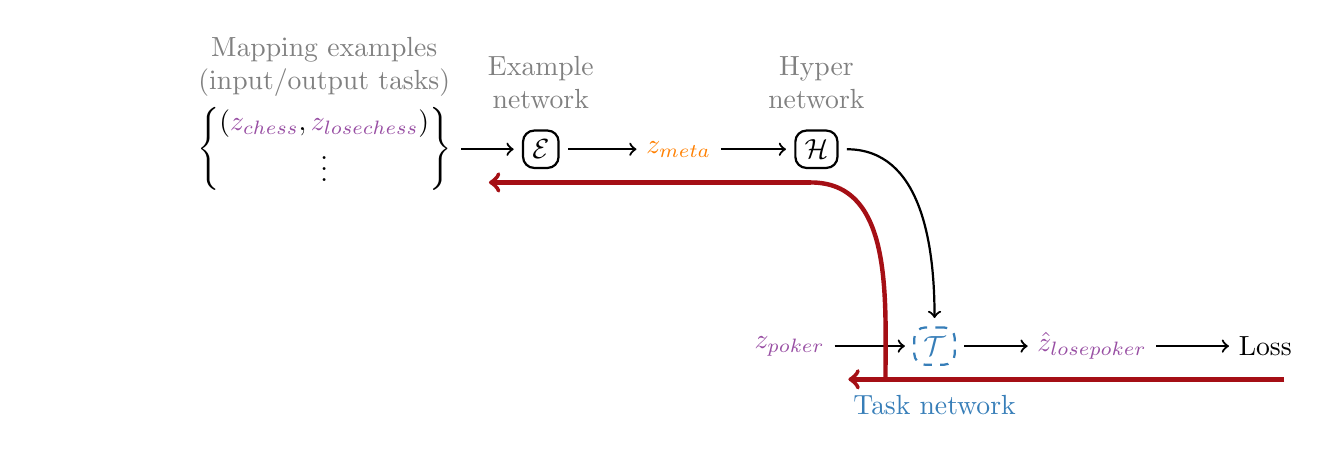
\begin{tikzpicture}[auto]
%% from examples
\node at (-6.9, 0) {};

\node[gray, text width=3.5cm, align=center] at (-3.25, 2.3) {Mapping examples (input/output tasks)};
\node at (-3.25, 1.25) (examples){
\(\left\{
\begin{matrix}
({\color{bpurp}z_{chess}}, {\color{bpurp}z_{lose chess}})\\
$\vdots$
\end{matrix}\right\}\)};

\node[gray, text width=2cm, align=center] at (-0.5, 2.1) {Example network};
\node[block] at (-0.5, 1.25) (examplenet) {\(\mathcal{E}\)};
\path[arrow] (examples.east) -- ([xshift=-3]examplenet.west);

%% performing 
\node[borange] at (1.25, 1.25) (taskrep) {\(z_{meta}\)};
\path[arrow] ([xshift=3]examplenet.east) -- (taskrep.west);

\node[gray, text width=2cm, align=center] at (3, 2.1) {Hyper network};
\node[block] at (3, 1.25) (hypernet) {\(\mathcal{H}\)};
\path[arrow] (taskrep.east) -- ([xshift=-3]hypernet.west);

\node[bpurp] at (2.66, -1.25) (handrep) {\(z_{poker}\)};

\node[bblue, block, dashed] at (4.5, -1.25) (tasknet) {\(\mathcal{T}\)};
\node[bblue, text width=3cm, align=center] at (4.5, -2) {Task network};
\path[arrow] (handrep.east) -- ([xshift=-3]tasknet.west);
\path[arrow, out=0, in=90] ([xshift=3]hypernet.east) to ([yshift=3]tasknet.north);

\node[bpurp] at (6.5, -1.25) (output) {\(\hat{z}_{lose poker}\)};
\path[arrow] ([xshift=3]tasknet.east) -- (output.west);

\node at (8.7, -1.25) (loss) {Loss};
\path[arrow] (output.east) -- (loss.west);

% gradients

\path[arrow, bred, ultra thick] ([yshift=-12, xshift=20]loss.west) to ([yshift=-12, xshift=5]handrep.east);

\path[draw, bred, ultra thick, out=90, in=0] ([yshift=-12, xshift=-10]tasknet.west) to ([yshift=-12, xshift=-10]hypernet.east);

\path[arrow, bred, ultra thick] ([yshift=-12, xshift=-10]hypernet.east) to ([yshift=-12, xshift=10]examples.east);
\end{tikzpicture}
}
\caption{Meta-mapping inference/training (from examples).}\label{supp_fig:HoMM:gradient_flow:meta_mappings}
\end{subfigure}
\caption[Schematic of architecture, showing inference and gradient flow through the model on a training step.]{Schematic of architecture, showing inference and gradient flow through the model on a training step. Thin black lines moving rightward represent inference, thick red lines moving leftward represent gradients. (\subref{supp_fig:HoMM:gradient_flow:basic_tasks}) Inference and gradients for the basic tasks. (\subref{supp_fig:HoMM:gradient_flow:basic_tasks}) Inference and gradients for meta-mappings. The gradients end at the examples of the meta-mapping, rather than propagating through to alter how those representations are constructed, due to GPU memory constraints. In the future, it might be useful to explore whether allowing further propagation would improve results for both basic tasks and meta-mappings. (These figures depict the inference/gradient flow when performing tasks and meta-mappings from examples, performing from language is similar, except that the example inputs and example network are replaced with language inputs and the language processing network.)} \label{supp_fig:HoMM:gradient_flow}
\end{figure}

In Fig. \ref{supp_fig:HoMM:gradient_flow}, we show the flow of inference (forward) and gradients (backward) through the HoMM architecture on basic task and meta-mapping training steps.

\begin{table}
\scriptsize
\centering
\begin{tabular}{|p{3cm}||c|c|c|c|}
\hline
& Polynomials & Cards & Visual & RL \\\hline
\hline
$Z$-dimension & 512 & 512 & 512 & 512 \\\hline
$\mathcal{I}$ num. layers & \multicolumn{4}{c|}{2} \\\hline
$\mathcal{I}$ num. hidden units & \multicolumn{4}{c|}{128} \\\hline
$\mathcal{I}$ conv. layers. (num filters, size, all strides are 2) & \multicolumn{2}{c|}{-} & \multicolumn{1}{p{2.3cm}|}{(64, 5), (128, 4), (256, 4), (512, 2), max pool} & \multicolumn{1}{p{2.3cm}|}{(64, 7), (64, 4), (64, 3)}\\\hline
$\mathcal{L}$ architecture & -  & \multicolumn{3}{c|}{2-layer LSTM + 2 fully-connected} \\\hline
$\mathcal{L}$ num. hidden units & -  & \multicolumn{3}{c|}{512} \\\hline
$\mathcal{T}$ num. layers & 1 & 3 & 1 & 3 \\\hline
$\mathcal{T}$ num. hidden units & - & 128 & - & 128 \\\hline
$\mathcal{E}$ architecture & \multicolumn{4}{c|}{2 layers per-datum, max pool across, 2 layers} \\\hline
$\mathcal{H}$ architecture & \multicolumn{4}{c|}{4 layers} \\\hline
$\mathcal{E}$ num. hidden units & \multicolumn{3}{c|}{512} & 1024 \\\hline
$\mathcal{H}$ num. hidden units & \multicolumn{4}{c|}{512} \\\hline
Task, MM representations from & \multicolumn{2}{c|}{Examples} & Language & Examples \\\hline
$\mathcal{F}$ num. layers & 3 & 1 & HoMM: 1, Lang: 3 & 3 \\\hline
$\mathcal{F}$ num. hidden units & \multicolumn{3}{c|}{64} & 128 \\\hline
$\mathcal{F}$ init scale & 1 & 1 & 30 & 10 \\\hline
$\mathcal{F}$ weight norm. \citep{Salimans2016} & \multicolumn{3}{c|}{No} & Yes \\\hline
$\mathcal{A}$ num. layers & \multicolumn{2}{c|}{1} & 2 & 1 \\\hline
$\mathcal{A}$ num. hidden units & \multicolumn{2}{c|}{-} & 128 & -  \\\hline
Nonlinearities & \multicolumn{4}{p{11cm}|}{Leaky ReLU most places, except no non-linearity at final layer of networks outputting to $Z$, sigmoid for classification outputs, and softmax over actions.} \\\hline
Base task loss & $\ell_2$ & $\ell_2$ (masked) & Cross-entropy & $\ell_2$ (masked)\\\hline
Meta-mapping loss & \multicolumn{4}{c|}{$\ell_2$}\\\hline
Partially-persistent task embeddings & \multicolumn{3}{c|}{No} & Yes \\\hline
Persistent embedding match loss weight & \multicolumn{3}{c|}{-} & 0.2 \\\hline
\hline
Optimizer & Adam & \multicolumn{3}{c|}{RMSProp} \\\hline
Learning rate (base) & $3\cdot 10^{-5}$ & $1\cdot 10^{-5}$ & $3\cdot 10^{-5}$ & $1\cdot 10^{-4}$\\\hline
Learning rate (meta) & $1\cdot 10^{-5}$ & $1\cdot 10^{-5}$ & $1\cdot 10^{-5}$ & $1\cdot 10^{-4}$\\\hline
L.R. decay rate (base) & $\times0.85$ & $\times0.85$ & $\times0.8$ & $\times0.8$\\\hline
L.R. decay rate (meta) & $\times0.85$ & $\times0.9$ & $\times0.85$ & $\times0.95$ \\\hline
L.R. min (base) & \multicolumn{2}{c|}{$3 \cdot 10^{-8}$}  & $1 \cdot 10^{-8}$ & $3 \cdot 10^{-8}$\\\hline
L.R. min (meta) & $1 \cdot 10^{-7}$& $3 \cdot 10^{-8}$ &  $1 \cdot 10^{-8}$ & $3 \cdot 10^{-7}$\\\hline
L.R. decays every & 100 epochs & 200 epochs & 400 epochs & 10000 \\\hline
Num. training epochs & 5000 & \multicolumn{1}{p{2.3cm}|}{100000 (optimally stopped)} & \multicolumn{1}{p{2.3cm}|}{10000 for 4 train mappings, 7500 for 8, 5000 for others} & \multicolumn{1}{p{2.3cm}|}{300000 (optimally stopped)} \\\hline
Num. runs & 5 & 5 & 10 & 5 \\ \hline
\hline
Num. base tasks (training) & \multicolumn{1}{p{2.3cm}|}{1300 ( $= 60 + 60 \times  20 + 40$)} & 36 & Varies & 18 \\\hline
Num. base tasks (held out for MM eval) & 800 ($= 40 \times 20$)  & 4 & Varies & 2 \\\hline
Num. meta classifications & 6 & 8 & 8 & - \\\hline
Num. train MMs & 20 & 3 & Varies & 1 \\\hline
Num. held-out MMs & 16 & 0 & 2 & 0  \\\hline
Base dataset size & 1024 & 1024 & 336 & 64 \\\hline
Base examples size & 50 & 768 & - & 32 \\\hline
Meta dataset size (train) & 60 & 36 & Varies & 18 \\\hline
Meta examples (train) & \multicolumn{2}{c|}{Half of train dataset} & - & Half of train dataset \\\hline
Meta examples (eval) & \multicolumn{2}{c|}{All of train dataset} & - & All of train dataset \\\hline
Base datasets refreshed & \multicolumn{2}{c|}{Every 50 epochs} & Every 20 & Every 1500  \\\hline
Target network updated & \multicolumn{3}{c|}{-} & Every 10000 epochs  \\\hline
RL discount & \multicolumn{3}{c|}{-} & 0.85 \\\hline
RL explore prob. (\(\epsilon\)) & \multicolumn{3}{c|}{-} & \multicolumn{1}{p{2.5cm}|}{Init: 1, decay: -0.03}\\\hline
Action softmax \(\beta\) & - & 8 & - & 8\\\hline
\end{tabular}
\caption[Detailed hyperparameter specification.]{Detailed hyperparameter specification for different experiments. A ``-'' indicates a parameter that does not apply to that experiment. As a reminder: the shared representational space is denoted by $Z$. Input encoder: $\mathcal{I}: \text{input} \rightarrow Z$. Action decoder $\mathcal{A}: Z \rightarrow \text{output}$. Target encoder $\mathcal{T}: \text{targets} \rightarrow Z$. Meta-network $\mathcal{E}: \{(Z, Z), ...\} \rightarrow Z $ maps examples to a task representation. Hyper-network $\mathcal{H}: Z \rightarrow \text{parameters}$. Task network $F: Z \rightarrow Z$ is parameterized by $\mathcal{H}$. Language encoder: $\mathcal{L}: \text{language} \rightarrow Z$. } \label{supp_hyperparameter_table}
\end{table}
See table \ref{supp_hyperparameter_table} for detailed architectural description and hyperparameters for each experiment. Hyperparameters were generally found by a heuristic search, where mostly only the optimizer, learning rate annealing schedule, and number of training epochs were varied. Some of the parameters take the values they do for fairly arbitrary reasons, e.g. the polynomial experiments were run earlier, before 1-layer task networks were found to be useful in some settings. While it would be ideal to fully search the space of parameters for all models, unfortunately our computational resource limitations prohibited it. Thus the results in the paper should be interpreted as a lower bound on what would be possible. \par
Each epoch consisted of a separate learning step on each task (both base and meta), in a random order. In each task, the meta-learner would receive only a subset (the ``batch size`` above) of the examples to generate a function embedding, and would have to generalize to the remainder of the examples in the dataset. The embeddings of the basic tasks used for meta-mappings were computed and cached once per epoch, so as the network learned over the course of the epoch, these task-embeddings would get ``stale,'' but this did not seem to be too detrimental. In the case of the RL tasks, where there were persistent task embeddings, they were used insteadd.\par
The results reported in the figures in this paper are averages across multiple runs, with different trained and held-out tasks (in the polynomial and visual concepts cases) and different network initializations and training orders each epoch (in all cases), to ensure the robustness of the findings. \par

\subsubsection{Source repositories}
%The full code for all experiments and analyses will be made available via github in the de-anonymized verison.
The full code for the experiments and analyses can be found on github:
\begin{itemize}
\item HoMM library: \url{https://github.com/lampinen/HoMM}
%\item This paper's source: \url{https://github.com/lampinen/metamapping_paper}
\item Polynomials: \url{https://github.com/lampinen/HoMM_polynomial_analysis}
\item Cards (models): \url{https://github.com/lampinen/HoMM_cards}
\item Cards (human experiment): \url{https://github.com/lampinen/cards_for_humans}
\item Concepts: \url{https://github.com/lampinen/categorization_HoMM}
\item RL: \url{https://github.com/lampinen/HoMM_grids}
\item Stroop results (below): \url{https://github.com/lampinen/stroop}
\end{itemize}



\section{Clarifying meta-mapping} \label{app_clarifying_meta_mapping}
\subsection{A definitional note}
When we discussed meta-mappings in the main text, we equivocated between tasks and behaviors for the sake of brevity. For a perfect model, this is somewhat justifiable, because each task will have a corresponding optimal behavior, and the sytem's embedding of the task will be precisely the embedding which produces this optimal behavior. However, behavior-irrelevant details of the task, like the color of the board, may not be embedded, so this should not really be thought of as a task-to-task mapping. This problem is exacerbated when the system is imperfect, e.g. during learning. It is thus more precise to distinguish between a ground-truth meta-mapping, which maps tasks to tasks, and the computational approach to achieving that meta-mapping, which really maps between representations which combine both task and behavior. \par



\chapter{Supplemental material for Chapter \getrefnumber{chapter:zero_shot_via_homm}} \label{appendix:zero_shot_via_homm}

\section{Details of polynomial task domain} \label{app:HoMM:polynomials_methods}
We randomly sampled the train and test polynomials as follows:
\begin{enumerate}
\item Sample the number of relevant variables ($k$) uniformly at random from 0 (i.e. a constant) to the total number of variables.
\item Sample the subset of $k$ variables that are relevant from all the variables.
\item For each term combining the relevant variables (including the intercept), include the term with probability 0.5. If so give it a random coefficient drawn from $\mathcal{N}(0, 2.5)$.
\end{enumerate}
The data points on which these polynomials were evaluated were sampled uniformly from $[-1, 1]$ independently for each variable, and for each polynomial. The datasets were resampled every 50 epochs of training. \par
\textbf{Meta-tasks:} For meta-tasks, we trained the network on 6 task-embedding classification tasks:
\begin{itemize}
\item Classifying polynomials as constant/non-constant.
\item Classifying polynomials as zero/non-zero intercept.
\item For each variable, identifying whether that variable was relevant to the polynomial.
\end{itemize}
We trained on 20 meta-mapping tasks, and held out 16 related meta-mappings.
\begin{itemize}
\item Squaring polynomials (where applicable).
\item Adding a constant (trained: -3, -1, 1, 3, held-out: 2, -2).
\item Multiplying by a constant (trained: -3, -1, 3, held-out: 2, -2).
\item Permuting inputs (trained: 1320, 1302, 3201, 2103, 3102, 0132, 2031, 3210, 2301, 1203, 1023, 2310, held-out: 0312, 0213, 0321, 3012, 1230, 1032, 3021, 0231, 0123, 3120, 2130, 2013).
\end{itemize}


%\section{Card game $t$-SNE} \label{app_cards_tsne}
%We performed $t$-SNE \citep{LaurensvanderMaaten2008} on the task embeddings of the system at the end of learning the card game tasks, to evaluate the organization of knowledge in the network. In fig. \ref{fig_cards_tsne_basic} we show these embeddings for just the basic tasks. The embeddings show systematic grouping by game attributes. In fig. \ref{fig_cards_tsne_full} we show the embeddings of the meta and basic tasks, showing the organization of the meta-tasks by type. (Note: this analysis was performed in an older version of the model than the main results.)\par 
%\begin{figure}[H]
%\centering
%\includegraphics[width=0.8\textwidth]{2-HoMM/figures/basic_tsne_basic_final.png}
%\caption{$t$-SNE embedding of the function embeddings the system learned for the basic card game tasks. (Note that the pairs of nearby embeddings differ in the ``suits rule`` attribute, discussed in appendix \ref{meth_data_cards}.)} 
%\label{fig_cards_tsne_basic}
%\end{figure}%
%\begin{figure}[H]
%\centering
%\includegraphics[width=0.9\textwidth]{2-HoMM/figures/basic_tsne_full_final.png}
%\caption{$t$-SNE embedding of the function embeddings the system learned for the meta tasks (basic tasks are included in the background).} 
%\label{fig_cards_tsne_full}
%\end{figure}

\section{Architecture \& training experiments} \label{app_lesion_results}
In this section we consider a few variations of the architecture and training, to justify the choices made in the paper. \par

\subsection{Inadequacy of vector analogies for meta-mapping} \label{supp_sec:HoMM:vector_analogies_inadequate}

One possible implementation of meta-mapping would be to just construct an analogy vector and use that for the mapping. This idea is motivated by work showing that word vector representations often support vector analogical reasoning; for example if we denote the vector for the word king as \(\vec{v}_{king}\), relationships like \(\vec{v}_{queen} \approx \vec{v}_{king} + \left(\vec{v}_{man} - \vec{v}_{woman} \right)\) often hold \citep{Mikolov2013}. Thus, adopting a similar strategy for meta-mapping would be superficially plausible. For example, in the polynomials domain, the meta-mapping ``Permute \((w, z, x, y)\)'' could be estimated by taking the vector differences between the representations of inputs and targets, computing an average difference vector, and adding that to the held-out examples to produce an output for each one.

However, in this section, we prove that such an approach cannot accurately represent all the meta-mappings in the polynomials domain. Furthermore, we sketch a proof by construction that a linear task network (i.e. an affine transformation, matrix multiplication plus a bias vector) parameterized independently for each meta-mapping suffices.

\textbf{Proof that vector analogies are inadequate:} In essence, the proof is simply that many of our meta-mappings are non-commutative, while vector addition is commutative. Consider the mappings for adding 1 to a polynomial, and multiplying by 2. Assume there were vector representations for these mappings, respectively \(\vec{m}_{+1}\) and \(\vec{m}_{\times 2}\). Let \(\vec{f}_{x}\) be the vector representation for the polynomial \(f(w,x,y,z) = x\). Then \(\vec{f}_{x} + \vec{m}_{+1} = \vec{f}_{x+1}\), \(\vec{f}_{x} + \vec{m}_{\times 2} = \vec{f}_{2x}\). But then:
\[ \vec{f}_{2(x + 1)} = \left(\vec{f}_{x} + \vec{m}_{+1}\right) + \vec{m}_{\times 2} = \vec{f}_{x} + \vec{m}_{+1} + \vec{m}_{\times 2} = \left(\vec{f}_{x} + \vec{m}_{\times 2}\right) + \vec{m}_{+1} = \vec{f}_{2x + 1}\]
Thus such a representation would result in contradictions, such as \(2x + 1 = 2x + 2\). Similar issues occur for permutation and other non-commutative mappings.

\textbf{Proof sketch that affine transformations in an appropriate vector space suffice:} Suppose that we have a vector representation for the polynomials, where there is a basis dimension corresponding to each monomial, so that the polynomial can be represented as a vector of its coefficients. (This is the standard vector-space representation for polynomials.) Then permutation corresponds to permuting these monomials, i.e. a permutation of the basis dimensions, which is a linear transformation. Adding a constant corresponds to adding to one dimension, which requires only the vector addition part of the affine transformation. Multiplying by a constant requires multiplying each dimension, i.e. a block-diagonal linear transformation.

Squaring polynomials is slightly more complex, and requires augmenting the vector space with components whose values are the product of the coefficients of each pair of monomials. In this case, squaring corresponds to a simple linear transformation. However, this augmentation makes the other meta-mappings more complex. The most difficult case is adding a constant, which requires shifting each pair term containing a constant by the product of the constant and the coefficient of the other monomial, but this again reduces to simply an appropriately parameterized affine transformation --- each pair term containing a constant term simply needs the added constant as a weight times the component for the other monomial. Thus affine transformations suffice in this setting.

Of course, with a sufficiently complex, deep, recurrent, and non-linear task network, any meta-mapping could be computed in principle, since a sufficiently complex network is Turing-complete \citep{Siegelman1992}. Thus, our approach to meta-mapping is fully general, conditioned on a sufficiently complex task network, while simpler approaches may not be.


\subsection{Basic meta-learning in the polynomials domain}

In Fig. \ref{supp_fig:HoMM:polynomials_basic_meta_learning}, we show that the basic meta-learning is working well in the cards domain. That is, we show that after the example network is presented with a set of example input, output pairs, the system is generalizing well to other points from that polynomial. At the end of training, the mean loss on trained polynomials is 0.025 (bootstrap 95\%-CI [0.02, 0.03]), and for held-out polynomials it is 0.58 (bootstrap 95\%-CI [0.45, 0.70]). Since chance loss is 11.76 for the trained polynomials, and 11.10 for the eval, this corresponds to about 99.8\% of optimal on the trained polynomials, and 94.8\% on the held-out.

\begin{figure}[H]
\centering
\includegraphics[width=0.66\textwidth]{2-HoMM/figures/basic_meta_learning_polynomials.png}
\caption[Basic meta-learning performance in the polynomials domain over learning.]{Basic meta-learning performance in the polynomials domain over learning. The system is generalizing at the meta-learning level. That is, this graph shows that, after the example network receives a set of (input, output) example tuples, it is generating a sufficiently good representation to regress held-out points from that polynomial. This is true both for polynomials it was trained with (green), and for polynomials that are held-out and never encountered during training (pink). (Thick lines are averages over 5 runs, shown as thin light curves.)} \label{supp_fig:HoMM:polynomials_basic_meta_learning}
\end{figure}

\subsection{Shared $Z$ vs. separate task-embedding and data-embedding space} \label{app_lesion_results_shared_z}
Instead of having a shared $Z$ where data and tasks are embedded, why not have a separate embedding space for data, tasks, and so on? There are a few conceptual reason why we chose to have a shared $Z$, including its greater parameter efficiency, the fact that humans seem to represent our conscious knowledge of different kinds in a shared space \citep[][]{Baars2005}, and the fact that this representation could allow for zero-shot adaptation to new computational pathways through the latent space, analogously to the zero-shot language translation results reported by Johnson and colleagues \citep{Johnson2016a}. In this section, we further show that training with a separate task encoding space worsens performance, see fig. \ref{supp_lesion_shared_z_fig}. This seems to primarily be due to the fact that learning in the shared $Z$ accelerates and de-noises the learning process, see fig. \ref{supp_lesion_shared_z_learn_fig}. (It's therefore worth noting that running this model for longer could result in convergence to the same asymptotic generalization performance.) Note: this analysis was performed in an older implementation of the model. \par
\begin{figure}[H]
\centering
\includegraphics[width=\textwidth]{2-HoMM/figures/poly/meta_results_unshared_vs_shared.png}
\caption[Having a separate embedding space for tasks results in worse performance on meta-mappings.]{Having a separate embedding space for tasks results in worse performance on meta-mappings. (Results are from only 1 run.)}
\label{supp_lesion_shared_z_fig}
\end{figure}

\begin{figure}[H]
\centering
\includegraphics[width=\textwidth]{2-HoMM/figures/poly/meta_learning_curves_with_separate.png}
\caption[Having a separate embedding space for tasks results in noisier, slower learning of meta-mappings.]{Having a separate embedding space for tasks results in noisier, slower learning of meta-mappings. (Results are from only 1 run.)}
\label{supp_lesion_shared_z_learn_fig}
\end{figure}

\subsection{Hyper network vs. conditioned task network} \label{app_lesion_results_hyper}
Instead of having the task network $F$ parameterized by the hyper network $\mathcal{H}$, we could simply have a task network with learned weights which takes a task embedding as another input. In Fig. \ref{supp_fig:HoMM_arch_cond_vs_hyper}, we show that this architecture fails to learn the meta-mapping tasks, although it can successfully perform the basic tasks. We suggest that this is because it is harder for this architecture to prevent interference between the comparatively larger number of basic tasks and the smaller number of meta-tasks. While it might be possible to succeed with this architecture, it was more difficult in the hyper-parameter space we searched. See also Fig. \ref{supp_fig:human:lang_tcnh}, where we show that both architectures perform similarly for language generalization. \par 

\begin{figure}[H]
\centering
\includegraphics[width=0.66\textwidth]{2-HoMM/figures/conditioned_vs_hyper_polynomials.png}
\caption[The HyperNetwork-based architecture we propose outperforms a simpler architecture.]{The HyperNetwork-based architecture we propose in the main text performs better and more consistently on meta-mappings than a simpler architecture that simply concatenates a task representation to the input before passing it through a fixed MLP. Results are in the polynomial domain, c.f. Fig. \ref{fig:HoMM_polynomials:results}. Note that the task-concatenated architecture performs just as well at the trained basic tasks (not shown), it is adapting via meta-mappings that proves challenging for it. See Supp. Fig. \ref{supp_fig:extending:RL:arch_cond_vs_hyper} for a more dramatic comparison in the RL domain. }\label{supp_fig:HoMM_arch_cond_vs_hyper}
\end{figure}

\subsection{Meta-classification lesion} \label{app:homm:metaclass_lesion}

In Fig. \ref{supp_fig:HoMM:metaclass_lesion}, we show that meta-classification training is not beneficial in the polynomials domain. Specifically, on trained meta-mappings the HoMM model is achieving a normalized performance of 88.99\% (bootstrap 95\%-CI [88.20, 89.98]), while without meta-classification it is achieving a normalized performance of 89.7\% (bootstrap 95\%-CI [88.87, 90.61]). On new meta-mappings the HoMM model is achieving a normalized performance of 85.54\% (bootstrap 95\%-CI [85.14, 85.94]), while without meta-classification it is achieving a normalized performance of 86.29\% (bootstrap 95\%-CI [85.54, 86.79]). While these differences are significant (paired \(t\)-tests, respectively \(t(4) = 6.95, p = 0.002\) and \(t(4) = 3.06, p = 0.038\)), the effect is small. See also Fig. \ref{supp_fig:human:homm_metaclass_lesion} for marginal evidence that meta-classification may be helpful in the cards domain, where there are fewer training tasks. 

\begin{figure}[H]
\centering
\includegraphics[width=0.66\textwidth]{2-HoMM/figures/metaclass_lesion_polynomials.png}
\caption[In the polynomials domain, the HoMM model performs slightly better without meta-classification training.]{In the polynomials domain, the HoMM model performs slightly better without meta-classification training. This effect appears for both trained and held-out meta-mappings. However, the effect is small.}\label{supp_fig:HoMM:metaclass_lesion}
\end{figure}


\chapter{Supplemental material for chapter \getrefnumber{chapter:human}} \label{appendix:human}

\section{Details of human experiment}
The experiment was implemented online, and run on Amazon Mechanical Turk. The code was based on the jsPsych library \citep{DeLeeuw2015}. The full code for the experiment and analysis can be found at \url{https://github.com/lampinen/cards_for_humans}. In this section we provide some details in a more easily readable format.

\subsection{Detailed experiment outline}

\subsubsection{Introduction \& rules}
\begin{itemize}
\item Page 1:
    \begin{itemize}
    \item Hi, welcome to our HIT. We are researchers from the Stanford Department of Psychology, conducting an experiment on game playing.
    \item The first part of this experiment should take 5-10 minutes. The base pay is \$1, and if you pass the end of the first phase, there will be a second phase that will take about 10 minutes. You will be paid a bonus of \$1.50 for making it to this second phase, there will be an extra bonus based on performance in the second phase.
    \item If you do not wish to participate, you may return the HIT at any time, but you will not be compensated unless you complete it.
    \end{itemize}
\item  Page 2:
    \begin{itemize}
    \item If you make it to the second phase of the experiment, you'll be playing a simple card game. In this first phase of the experiment, you'll learn the rules.
    \item We'll test your understanding of the rules at the end of the first phase, and if you pass you'll make it to the second phase, where you'll earn a \$1 bonus + an extra performance bonus.
    \item Make sure you follow all instructions very carefully, in order to make it to the second phase of the experiment and earn the maximum bonus pay.
    \end{itemize}
\item  Page 3:
    \begin{itemize}
    \item In the card game, you will receive a hand of two cards, each of which has a number (1-4) and a color (red or black). There are several decks in play, so there are multiple copies of each card, and two or more can appear in the same round.
    \end{itemize}
\item  Page 4:
    \begin{itemize}
    \item You will be playing against an opponent, trying to win money. You'll get to make a bet of 0, 5, or 10 cents.
    \item If your hand beats your opponent's hand, you will win the amount you bet. If your opponent wins, you'll lose the amount you bet. If you bet nothing, you won't win or lose anything. Also, if you tie, you won't win or lose either.
    \item In the second phase, we'll pay you a bonus equal to your net earnings (or 0 if your earnings are negative), on top of the \$1 bonus for making it to the second phase."
    \end{itemize}
\item  Page 5:
    \begin{itemize}
    \item In the card game, \textbf{the best types of hands are two adjacent numbers of the same color}, for example black 2 and black 3.
    \item \textbf{The next best hands are those with two adjacent numbers of different color,} for example black 3 and red 4.
    \item \textbf{The worst types of hands are those with matching numbers or non-adjacent numbers}, like 4, 4 or 1, 3.
    \item \textbf{Hands of better types always beat worse hands.}
    \end{itemize}
\item  Page 6:
    \begin{itemize}
    \item \textbf{If two hands are of the same type, the one with the highest card wins.} If the highest cards of the two hands tie, the tie is broken by the lower cards.
    \item \textbf{If both cards are tied, black cards beat red cards,} highest first, lowest if the high cards are the same color. If the hands are perfectly tied, you don't win or lose money.
    \end{itemize}
\end{itemize}

\subsubsection{Game understanding check}
\begin{itemize}
\item Instructions:
    \begin{itemize}
    \item We'll now test your understanding by giving you a few example pairs of hands. Just click on the hand from each pair that would win. \textbf{\color{red} If you make more than one mistake in this section, the experiment will end. Make sure you fully understand the instructions before proceeding, otherwise you may not make it to the second phase!}
    \item If you need to, you can go back to the earlier instructions to refresh your memory before proceeding.
    \item Click next to start the test.
    \end{itemize}
\item Trials (see fig. \ref{fig:appdx_human_comparison_trial}, hand position was randomized):
    \begin{itemize}
        \item black 3 and red 2 vs. red 4 and 1. Explanation: "Adjacent cards beat non-adjacent." 
        \item red 1 and 2 vs. red 4 and black 3. Explanation: "Same-suit adjacent beats different suit." 
        \item black 3 and red 3 vs. red 4 and 1. Explanation: "Highest card breaks ties." 
        \item black 4 and 3 vs. red 4 and 3. Explanation: "Black cards beat red cards if the numbers are tied." 
    \end{itemize}
\item Evaluation: If the participants got 3 out of 4 trials correct, they passed. 
    \begin{itemize}
        \item \textbf{Passed:} Congratulations, you passed the test, and will get to proceed to phase 2! You have earned a \$1.50 bonus, and will be awarded a performance bonus based on your bets in the next phase. Press any key to continue.
        \item \textbf{Failed:} Sorry, you made more than one mistake, and did not pass the test. The experiment will now end. Press any key to continue.
    \end{itemize}
\end{itemize}

\begin{figure}
\centering
\includegraphics[width=0.75\textwidth]{3-human-adaptation/figures/comparison_correct.png}
\caption{An example hand-comparison trial from the understanding check.} \label{fig:appdx_human_comparison_trial}
\end{figure}

\subsubsection{Block 1: with feedback}
\begin{itemize}
\item Instructions:
    \begin{itemize}
    \item Now you get to play a few hands. After you bet, we'll show you your opponent's hand and how much you won (or lost), and at the end of these hands we'll tell you your total earnings. Press any key to continue.
    \end{itemize}

\item Trials:
    \begin{itemize}
    \item 32 trials of playing the game and seeing the result of each hand, with the participants hand distributed evenly across 16 bins of hand win probability. Opponents hands were randomly sampled. 
    \end{itemize}
\item Block end:
    \begin{itemize}
    \item Participants were shown their block earnings, as well as their total earnings so far.
    \end{itemize}
\end{itemize}

\subsubsection{Block 2: without feedback}
\begin{itemize}
\item Instructions:
    \begin{itemize}
    \item To test how well you understand the game, we'll now give you a series of hands where you won't see your results after you bet. You will just see your earnings at the end of the set of hands. Press any key to continue.
    \end{itemize}
\item Trials:
    \begin{itemize}
    \item 24 trials of playing the game with the result grayed out, with the participants hand distributed evenly across 8 bins of hand win probability. Opponents hands were not sampled, participants were paid their expected earnings for each hand, with the final block total rounded to the closest 10 cents. 
    \end{itemize}
\item Block end:
    \begin{itemize}
    \item Participants were shown their block earnings, as well as their total earnings so far.
    \end{itemize}
\end{itemize}

\subsubsection{Block 3: losing variation, no feedback}
\begin{itemize}
\item Instructions:
    \begin{itemize}
    \item \textbf{\color{red} Now, we want you to try to lose the game! For the remainder of the experiment, if you bet and lose, you'll gain the amount you bet, and if you bet and win, you'll lose the amount you bet.}
    \item As before, you won't win or lose anything if you tie your opponent, or if you don't bet.
    \item Press any key to continue.
    \end{itemize}
\item Attention check:
    \begin{itemize}
    \item To make sure you understand, please answer this question. From now on, I will earn money if I:
    \item ``Bet and my hand wins.'', ``Bet and my hand loses.'' 
    \end{itemize}
\item Instructions 2:
    \begin{itemize}
    \item Great, now you get to play a few hands! As before, you won't see your results after you bet. You will just see your earnings at the end of the set of hands. Press any key to continue.
    \end{itemize}
\item Trials:
    \begin{itemize}
    \item 24 trials of playing the game with the result grayed out, with the participants hand distributed evenly across 8 bins of hand win probability. Opponents hands were not sampled, participants were paid their expected earnings for each hand, with the final block total rounded to the closest 10 cents. 
    \end{itemize}
\item Block end:
    \begin{itemize}
    \item Participants were shown their block earnings, as well as their total earnings so far.
    \end{itemize}
\end{itemize}

\subsubsection{Debrief}
We asked participants about their age, education, gender, and race/ethnicity. However, we did not analyze these data.


\section{Details of model tasks \& training}\label{app:human:model_details}
\subsection{Tasks}

Our card games were played with two suits, and 4 values per suit. In our setup, each hand in a game has a win probability (proportional to how it ranks against all other possible hands). The agent is dealt a hand, and then has to choose to bet 0, 1, or 2 (the three actions it has available). We considered a variety of games which depend on different features of the hand:
\begin{itemize}
\item \textbf{Straight flush:} Most valuable is adjacent numbers in same suit, i.e. 4 and 3 in most valuable suit (royal flush) wins against every other hand. This is the game we tested in human participants.
\item \textbf{High card:} Highest card wins.
\item \textbf{Pairs} Same as high card, except pairs are more valuable, and same suit pairs are even more valuable.
\item \textbf{Match:} The hand with cards that differ least in value (suit counts as 0.5 pt difference) wins.
\item \textbf{Blackjack:} The hand's value increases with the sum of the cards until it crosses 5, at which point the player ``goes bust,'' and the value becomes negative.
\end{itemize}
We also considered three binary attributes that could be altered to produce variants of these games:
\begin{itemize}
\item \textbf{Losers:} Try to lose instead of winning! Reverses the ranking of hands. This is the mapping we evaluated in human participants.
\item \textbf{Suits rule:} Instead of suits being less important than values, they are more important (essentially flipping the role of suit and value in most games).
\item \textbf{Switch suit:} Switches which of the suits is more valuable.
\end{itemize}
Any combination of these options can be applied to any of the 5 games, yielding 40 possible games. \par

\subsection{Training}
\textbf{Meta-mappings:} We trained the network on meta-mappings that toggled each of the binary attributes, but evaluated primarily on switching to losing the Straight Flush game (since that corresponded to the human experiment).\par
\textbf{Meta-classifications:} For meta-tasks, we gave the network 8 task-embedding classification tasks (one-vs-all classification of each of the 5 game types, and of each of the 3 attributes) \par
\textbf{Language:} We encoded the tasks in language by sequences of the form\\
\verb|[``game'', <game_type>, ``losers'', <losers-value>, ``suits rule'', <suits-rule-value>,|\\
\verb|``switch suit'', <switch-suit-value>]|.



\section{Supplementary analyses}
\subsection{Human suboptimality}\label{appendix:human:suboptimality}
As \citet{Jarvstad2013} note, how ``optimal'' human performance seems to be depends on how you measure performance. In particular, performance seems better when measured in terms of expected earnings than when measured in terms of how accurately participants decided whether or not to bet (fig. \ref{fig:appx_human_calibration}). This is because the participants were more accurate on trials with higher (absolute) expected value, and less accurate on trials where they had less to gain or lose. We chose the more optimistic performance measure as the basis for our comparison to the HoMM model.
\begin{figure}[H]
\centering
\begin{subfigure}[t]{0.5\textwidth}
\includegraphics[width=\textwidth]{3-human-adaptation/figures/human_adaptation_supp_earnings.png}
\caption{Performance measured in terms of earnings.}
\end{subfigure}%
\begin{subfigure}[t]{0.5\textwidth}
\includegraphics[width=\textwidth]{3-human-adaptation/figures/human_adaptation_supp_accuracy.png}
\caption{Performance measured in terms of accuracy, i.e. the percent of hands where an optimal decision was made}
\end{subfigure}%
\caption{How optimal human performance appears depends on the metric used to evaluate it.} \label{fig:appx_human_calibration}
\end{figure}

\subsection{Comparing to a simpler architecture for language generalization}\label{appendix:human:lang_tcnh}
In Fig. \ref{supp_fig:human:lang_tcnh} we show that language generalization is comparable in the HyperNetwork-based architecture we used for HoMM and a simpler architecture which simply concatenates the task representation to the input representation before passing them through a fixed feed-forward task network. Specifically, the HyperNetwork architecture achieves a mean expected reward of 1.79\% (bootstrap 95\%-CI [-12.31, 15.88]), while the simpler architecture achieves a mean expected reward of -8.59\% (bootstrap 95\%-CI [-20.42, -0.99]). See Supp. Figs. \ref{supp_fig:HoMM_arch_cond_vs_hyper} and \ref{supp_fig:extending:RL:arch_cond_vs_hyper} for the same architecture comparison for HoMM itself.  

\begin{figure}[H]
\centering
\includegraphics[width=0.66\textwidth]{3-human-adaptation/figures/cards_lang_hyper_vs_tcnh.png}
\caption[Language generalization is similar in the cards domain with either the HyperNetwork architecture used by HoMM, or a simpler task-concatenated architecture.]{Language generalization is similar in the cards domain with either the HyperNetwork architecture used by HoMM, or a simpler task-concatenated architecture. Compare to Fig. \ref{fig:human_cards_homm_results} for the human and HoMM results.} \label{supp_fig:human:lang_tcnh}
\end{figure}

\subsection{HoMM without meta-classification}

In Fig. \ref{supp_fig:human:homm_metaclass_lesion} we show that the HoMM model may be performing slightly better with meta-classification training than without it, although the difference is only marginally significant (paired \(t\)-test, \(t(4) = 2.23, p = 0.09\)). Specifically, the HoMM model is achieving an average expected reward of 85.38\% (bootstrap 95\%-CI [79.49, 90.32]), while without meta-classification it is achieving an average expected reward of 78.68\% (bootstrap 95\%-CI [71.01, 85.97]). See Fig. \ref{supp_fig:HoMM:metaclass_lesion} for a similar comparison in the polynomials domain, and meta-classification may be deleterious (possibly because there are many more training tasks, so it is not needed). 

\begin{figure}[H]
\centering
\includegraphics[width=0.66\textwidth]{3-human-adaptation/figures/cards_metaclass_lesion.png}
\caption[The HoMM model performs marginally worse without meta-classification training.]{The HoMM model performs marginally worse without meta-classification training. Thus this training may allow the model to adapt more robustly to new tasks.} \label{supp_fig:human:homm_metaclass_lesion}
\end{figure}

\chapter{Supplemental material for Chapter \getrefnumber{chapter:extending}} \label{appendix:extending}

\section{RL tasks} \label{app:extending_grids_methods}

All implementation and analysis code can be found at \url{https://github.com/lampinen/HoMM_grids}.\par


\subsection{Correlation in generalization across tasks}
In Fig. \ref{fig:app_extending:RL_correlation_by_run}, we show the correlation in performance on the pick-up and push-off generalization tasks within each run (at different time points in learning). Points are only included if train performance is above the threshold used for selection --- \(3.8\) for the HoMM model, \(3.5\) for the language model. Stricter thresholds for the language model result in weaker (sometimes negative) correlations (not shown). \par 
\begin{figure}
\centering
\includegraphics[width=\textwidth]{4-extending/figures/grids_adaptation_correlation_loose_by_run.png}
\caption[Correlation of performance on the RL tasks, by run.]{Correlation of performance on the two RL tasks, broken down by run. The correlation is higher in the HoMM model, both within and across runs.} \label{fig:app_extending:RL_correlation_by_run}
\end{figure}


\subsection{HyperNetwork-based architecture}
In Fig. \ref{supp_fig:extending:RL:arch_cond_vs_hyper}, we show that the HyperNetwork-based architecture outperforms a task-network-concatenating architecture at meta-mapping on the RL tasks, as in the polynomials domain. \par 

\begin{figure}
\centering
\includegraphics[width=0.8\textwidth]{4-extending/figures/grids_hyper_vs_tcnh.png}
\caption[In the RL domain, the HyperNetwork-based architecture performs better on meta-mappings than an architecture that simply concatenates a task representation to the input.]{In the RL domain, the HyperNetwork-based architecture performs better on meta-mappings than an architecture that simply concatenates a task representation to the input before passing it through a fixed MLP. We showed similar (though less dramatic) results for the polynomials domain in Supp. Fig. \ref{supp_fig:HoMM_arch_cond_vs_hyper}}\label{supp_fig:extending:RL:arch_cond_vs_hyper}
\end{figure}


\section{Categorization tasks} \label{app:extending_categorization_methods}
All implementation and analysis code can be found at \url{https://github.com/lampinen/categorization_HoMM}.\par
In Fig. \ref{fig:app_extending_cat_stims} we show all shapes (triangle, square, plus, circle, tee, inverseplus, emptysquare, emptytriangle), colors (blue, pink, purple, yellow, ocean, green, cyan, red), and sizes (16, 24, and 32 pixels) that we used in our experiments. All stimuli were rendered at random positions within a \(50 \times 50\) image (constrained so that the full shape remained within the frame), and at random angles within \(\pm20^{\circ}\) of their canonical orientation.\par

\begin{figure}[!htb]
\centering
\begin{subfigure}{0.24\textwidth}
\includegraphics[width=\textwidth]{4-extending/figures/categorization_stimuli/16_blue_triangle.png}
\end{subfigure}%
\begin{subfigure}{0.24\textwidth}
\includegraphics[width=\textwidth]{4-extending/figures/categorization_stimuli/24_pink_square.png}
\end{subfigure}%
\begin{subfigure}{0.24\textwidth}
\includegraphics[width=\textwidth]{4-extending/figures/categorization_stimuli/32_purple_plus.png}
\end{subfigure}%
\begin{subfigure}{0.24\textwidth}
\includegraphics[width=\textwidth]{4-extending/figures/categorization_stimuli/16_cyan_emptysquare.png}
\end{subfigure}\\
\begin{subfigure}{0.24\textwidth}
\includegraphics[width=\textwidth]{4-extending/figures/categorization_stimuli/24_ocean_tee.png}
\end{subfigure}%
\begin{subfigure}{0.24\textwidth}
\includegraphics[width=\textwidth]{4-extending/figures/categorization_stimuli/32_green_inverseplus.png}
\end{subfigure}%
\begin{subfigure}{0.24\textwidth}
\includegraphics[width=\textwidth]{4-extending/figures/categorization_stimuli/16_yellow_circle.png}
\end{subfigure}%
\begin{subfigure}{0.24\textwidth}
\includegraphics[width=\textwidth]{4-extending/figures/categorization_stimuli/24_red_emptytriangle.png}
\end{subfigure}%
\caption{Sample stimuli for categorization tasks, showing all shapes, colors, and sizes.} \label{fig:app_extending_cat_stims}
\end{figure}

\subsection{Language model architecture} \label{app:extending_categorization_lang_arch}

In the categorization experiments, we used a different task network architecture for the meta-mapping based architectures than for the language generalization architectures. Here, we justify that choice by showing that the model architecture we used for the meta-mapping approach results in worse language generalization, in Fig. \ref{fig:app_extending_cat_lang_arch}. In particular, the linear task network resulted in worse generalization performance (mean \(= 0.85\), bootstrap 95\%-CI [0.82, 0.88]) than the deep nonlinear task network (mean \(= 0.92\), bootstrap 95\%-CI [0.89, 0.94]). This difference was significant under a linear mixed-model (\(t(4) = 3.615\), \(p = 0.02\)), and under a permutation test. \par 

\begin{figure}
\includegraphics[width=0.8\textwidth]{4-extending/figures/language_model_architecture_justification.png}
\caption[Comparing language generalization with linear vs. deep-nonlinear task-networks.]{Comparing language generalization with a linear task network to a deep, nonlinear architecture. Although the linear task network worked best for the meta-mapping approaches (not shown), the nonlinear task network generalized better to new language instructions.} \label{fig:app_extending_cat_lang_arch}
\end{figure}

\subsection{More detailed result visualizations}
In Fig. \ref{fig:app_extending:concepts_generalization_density} we show the zero-shot generalization accuracy of the models across runs, at different training set sizes. At moderate sample sizes, the HoMM model results in a sharper peak at perfect accuracy --- i.e. more qualitatively ``getting it'' or ``not getting it.'' \par 
In Fig. \ref{fig:app_extending:concepts_all_runs} we show learning curves for meta-mapping performance across all runs. Performance is highly variable at small training-set sizes, especially on held-out meta-mappings, but becomes increasingly systematic as training set size increases.\par

\begin{figure}[H]
\centering
\includegraphics[width=0.5\textwidth]{4-extending/figures/concepts_adaptation_generalization_density.png}
\caption[Visual concept generalization densities.]{In the visual concepts domain, meta-mapping results in more qualitative ``getting it'' or ``not getting it'' behavior, in the middle ranges of dataset size. Here we plot the density of the zero-shot evaluation accuracy across runs for the HoMM model and language generalization. The HoMM model exhibits sharper peaking at one at moderate sample sizes, whereas the language generalization is more smeared out --- i.e. the HoMM model is either systematically getting everything correct or is making a large number of mistakes, whereas the language generalization is more stochastic. This qualitative, systematic difference in performance that HoMM exhibits is more like what would be expected from human cognition.}\label{fig:app_extending:concepts_generalization_density}
\end{figure}

\begin{figure}[p]
\centering
\begin{subfigure}{\textwidth}
\centering
\includegraphics[width=0.88\textwidth]{4-extending/figures/concepts_all_runs_train.png}
\caption{Trained meta-mappings.}\label{fig:app_extending:concepts_all_runs:train}
\end{subfigure}\\
\begin{subfigure}{\textwidth}
\centering
\includegraphics[width=0.88\textwidth]{4-extending/figures/concepts_all_runs_eval.png}
\caption{Held-out meta-mappings.}\label{fig:app_extending:concepts_all_runs:eval}
\end{subfigure}
\caption[Visual concept learning curves by run.]{Meta-mapping learning curves in the visual concepts domain broken down by number of training meta-mappings (rows), and by run (columns). The green lines are performance when the transformed task was encountered during training, the pink lines are performance on transformed tasks that were never encountered during training. Panel (\subref{fig:app_extending:concepts_all_runs:train}) shows the results for trained meta-mappings, and panel (\subref{fig:app_extending:concepts_all_runs:eval}) shows the results for held-out meta-mappings. With more training meta-mappings, HoMM both generalizes better when applying the trained meta-mappings to held-out examples (\subref{fig:app_extending:concepts_all_runs:train}), and when applying held-out meta-mappings (\subref{fig:app_extending:concepts_all_runs:eval}). However, even with smaller sample sizes, HoMM is achieving perfect generalization on the trained meta-mappings on many runs.} \label{fig:app_extending:concepts_all_runs}
\end{figure}



\addcontentsline{toc}{chapter}{Bibliography}
\bibliographystyle{apalike}
\bibliography{arrr}

\end{document}
